\documentclass[twoside]{book}

% Packages required by doxygen
\usepackage{fixltx2e}
\usepackage{calc}
\usepackage{doxygen}
\usepackage[export]{adjustbox} % also loads graphicx
\usepackage{graphicx}
\usepackage[utf8]{inputenc}
\usepackage{makeidx}
\usepackage{multicol}
\usepackage{multirow}
\PassOptionsToPackage{warn}{textcomp}
\usepackage{textcomp}
\usepackage[nointegrals]{wasysym}
\usepackage[table]{xcolor}

% NLS support packages
\usepackage[ngerman]{babel}

% Font selection
\usepackage[T1]{fontenc}
\usepackage[scaled=.90]{helvet}
\usepackage{courier}
\usepackage{amssymb}
\usepackage{sectsty}
\renewcommand{\familydefault}{\sfdefault}
\allsectionsfont{%
  \fontseries{bc}\selectfont%
  \color{darkgray}%
}
\renewcommand{\DoxyLabelFont}{%
  \fontseries{bc}\selectfont%
  \color{darkgray}%
}
\newcommand{\+}{\discretionary{\mbox{\scriptsize$\hookleftarrow$}}{}{}}

% Page & text layout
\usepackage{geometry}
\geometry{%
  a4paper,%
  top=2.5cm,%
  bottom=2.5cm,%
  left=2.5cm,%
  right=2.5cm%
}
\tolerance=750
\hfuzz=15pt
\hbadness=750
\setlength{\emergencystretch}{15pt}
\setlength{\parindent}{0cm}
\setlength{\parskip}{0.2cm}
\makeatletter
\renewcommand{\paragraph}{%
  \@startsection{paragraph}{4}{0ex}{-1.0ex}{1.0ex}{%
    \normalfont\normalsize\bfseries\SS@parafont%
  }%
}
\renewcommand{\subparagraph}{%
  \@startsection{subparagraph}{5}{0ex}{-1.0ex}{1.0ex}{%
    \normalfont\normalsize\bfseries\SS@subparafont%
  }%
}
\makeatother

% Headers & footers
\usepackage{fancyhdr}
\pagestyle{fancyplain}
\fancyhead[LE]{\fancyplain{}{\bfseries\thepage}}
\fancyhead[CE]{\fancyplain{}{}}
\fancyhead[RE]{\fancyplain{}{\bfseries\leftmark}}
\fancyhead[LO]{\fancyplain{}{\bfseries\rightmark}}
\fancyhead[CO]{\fancyplain{}{}}
\fancyhead[RO]{\fancyplain{}{\bfseries\thepage}}
\fancyfoot[LE]{\fancyplain{}{}}
\fancyfoot[CE]{\fancyplain{}{}}
\fancyfoot[RE]{\fancyplain{}{\bfseries\scriptsize Erzeugt am Mon Jan 12 2015 01\+:04\+:07 für Easy\+Set von Doxygen }}
\fancyfoot[LO]{\fancyplain{}{\bfseries\scriptsize Erzeugt am Mon Jan 12 2015 01\+:04\+:07 für Easy\+Set von Doxygen }}
\fancyfoot[CO]{\fancyplain{}{}}
\fancyfoot[RO]{\fancyplain{}{}}
\renewcommand{\footrulewidth}{0.4pt}
\renewcommand{\chaptermark}[1]{%
  \markboth{#1}{}%
}
\renewcommand{\sectionmark}[1]{%
  \markright{\thesection\ #1}%
}

% Indices & bibliography
\usepackage{natbib}
\usepackage[titles]{tocloft}
\setcounter{tocdepth}{3}
\setcounter{secnumdepth}{5}
\makeindex

% Hyperlinks (required, but should be loaded last)
\usepackage{ifpdf}
\ifpdf
  \usepackage[pdftex,pagebackref=true]{hyperref}
\else
  \usepackage[ps2pdf,pagebackref=true]{hyperref}
\fi
\hypersetup{%
  colorlinks=true,%
  linkcolor=blue,%
  citecolor=blue,%
  unicode%
}

% Custom commands
\newcommand{\clearemptydoublepage}{%
  \newpage{\pagestyle{empty}\cleardoublepage}%
}


%===== C O N T E N T S =====

\begin{document}

% Titlepage & ToC
\hypersetup{pageanchor=false,
             bookmarks=true,
             bookmarksnumbered=true,
             pdfencoding=unicode
            }
\pagenumbering{roman}
\begin{titlepage}
\vspace*{7cm}
\begin{center}%
{\Large Easy\+Set }\\
\vspace*{1cm}
{\large Erzeugt von Doxygen 1.8.9.1}\\
\vspace*{0.5cm}
{\small Mon Jan 12 2015 01:04:07}\\
\end{center}
\end{titlepage}
\clearemptydoublepage
\tableofcontents
\clearemptydoublepage
\pagenumbering{arabic}
\hypersetup{pageanchor=true}

%--- Begin generated contents ---
\chapter{Verzeichnis der Namensbereiche}
\section{Liste aller Namensbereiche}
Liste aller Namensbereiche mit Kurzbeschreibung\+:\begin{DoxyCompactList}
\item\contentsline{section}{\hyperlink{namespace_ui}{Ui} }{\pageref{namespace_ui}}{}
\end{DoxyCompactList}

\chapter{Hierarchie-\/\+Verzeichnis}
\section{Klassenhierarchie}
Die Liste der Ableitungen ist -\/mit Einschränkungen-\/ alphabetisch sortiert\+:\begin{DoxyCompactList}
\item \contentsline{section}{Card}{\pageref{class_card}}{}
\begin{DoxyCompactList}
\item \contentsline{section}{Card\+Widget}{\pageref{class_card_widget}}{}
\end{DoxyCompactList}
\item Q\+Main\+Window\begin{DoxyCompactList}
\item \contentsline{section}{Setup\+Window}{\pageref{class_setup_window}}{}
\item \contentsline{section}{Window}{\pageref{class_window}}{}
\end{DoxyCompactList}
\item Q\+Object\begin{DoxyCompactList}
\item \contentsline{section}{Packet\+Handler}{\pageref{class_packet_handler}}{}
\end{DoxyCompactList}
\item Q\+Tcp\+Server\begin{DoxyCompactList}
\item \contentsline{section}{Server}{\pageref{class_server}}{}
\begin{DoxyCompactList}
\item \contentsline{section}{Controller}{\pageref{class_controller}}{}
\end{DoxyCompactList}
\end{DoxyCompactList}
\item Q\+Tcp\+Socket\begin{DoxyCompactList}
\item \contentsline{section}{Client}{\pageref{class_client}}{}
\begin{DoxyCompactList}
\item \contentsline{section}{Player}{\pageref{class_player}}{}
\begin{DoxyCompactList}
\item \contentsline{section}{K\+I}{\pageref{class_k_i}}{}
\end{DoxyCompactList}
\end{DoxyCompactList}
\end{DoxyCompactList}
\item Q\+Widget\begin{DoxyCompactList}
\item \contentsline{section}{Card\+Widget}{\pageref{class_card_widget}}{}
\item \contentsline{section}{Information\+Widget}{\pageref{class_information_widget}}{}
\end{DoxyCompactList}
\end{DoxyCompactList}

\chapter{Klassen-\/\+Verzeichnis}
\section{Auflistung der Klassen}
Hier folgt die Aufzählung aller Klassen, Strukturen, Varianten und Schnittstellen mit einer Kurzbeschreibung\+:\begin{DoxyCompactList}
\item\contentsline{section}{\hyperlink{class_card}{Card} \\*Die Klasse \hyperlink{class_card}{Card} stellt das digitale pendant zu den analogen Karten des Spiels Set dar }{\pageref{class_card}}{}
\item\contentsline{section}{\hyperlink{class_card_widget}{Card\+Widget} \\*Die grafische Implementierung der Klasse \hyperlink{class_card}{Card} }{\pageref{class_card_widget}}{}
\item\contentsline{section}{\hyperlink{class_client}{Client} \\*Die abstrakte Klasse \hyperlink{class_client}{Client} kümmert sich um die Verbindung zum \hyperlink{class_server}{Server} und macht so ein Spielen möglich }{\pageref{class_client}}{}
\item\contentsline{section}{\hyperlink{class_controller}{Controller} \\*Die Klasse \hyperlink{class_controller}{Controller} ist für den kompletten Spielverlauf zuständig.~\newline
 Sie regelt, wann welcher \hyperlink{class_client}{Client} welche Pakete empfängt, wann das Spiel zu Ende ist/anfängt und~\newline
 wenn Karten nachgelegt werden sollen }{\pageref{class_controller}}{}
\item\contentsline{section}{\hyperlink{class_information_widget}{Information\+Widget} \\*Das \hyperlink{class_information_widget}{Information\+Widget} dient zur Ausgabe des Spielstatuses }{\pageref{class_information_widget}}{}
\item\contentsline{section}{\hyperlink{class_k_i}{K\+I} }{\pageref{class_k_i}}{}
\item\contentsline{section}{\hyperlink{class_packet_handler}{Packet\+Handler} \\*Die Packet\+Handler-\/\+Klasse dient zur Verwaltung von ein-\/ bzw. ausgehenden Paketen.~\newline
 Werden bestimmte Pakettypen erkannt, so werden die entsprechenden Signale emittiert,~\newline
 und dadurch die Slots in den externen Klassen aufgerufen }{\pageref{class_packet_handler}}{}
\item\contentsline{section}{\hyperlink{class_player}{Player} \\*Spieler-\/\+Klasse }{\pageref{class_player}}{}
\item\contentsline{section}{\hyperlink{class_server}{Server} \\*Die abstrakte Klasse \hyperlink{class_server}{Server}, steht für den \hyperlink{class_server}{Server} des Spiels }{\pageref{class_server}}{}
\item\contentsline{section}{\hyperlink{class_setup_window}{Setup\+Window} \\*Die Klasse \hyperlink{class_setup_window}{Setup\+Window} ist ein kleiner Einrichtungsassistent, um ein Spiel zu konfigurieren }{\pageref{class_setup_window}}{}
\item\contentsline{section}{\hyperlink{class_window}{Window} \\*Die Singleton-\/\+Klasse \hyperlink{class_window}{Window} ist die Haupt\+G\+U\+I.~\newline
 Dort findet das Spiel so wirklich für die Spieler statt }{\pageref{class_window}}{}
\end{DoxyCompactList}

\chapter{Datei-\/\+Verzeichnis}
\section{Auflistung der Dateien}
Hier folgt die Aufzählung aller Dateien mit einer Kurzbeschreibung\+:\begin{DoxyCompactList}
\item\contentsline{section}{src/\hyperlink{card_8cpp}{card.\+cpp} }{\pageref{card_8cpp}}{}
\item\contentsline{section}{src/\hyperlink{card_8hpp}{card.\+hpp} }{\pageref{card_8hpp}}{}
\item\contentsline{section}{src/\hyperlink{cardwidget_8cpp}{cardwidget.\+cpp} }{\pageref{cardwidget_8cpp}}{}
\item\contentsline{section}{src/\hyperlink{cardwidget_8hpp}{cardwidget.\+hpp} }{\pageref{cardwidget_8hpp}}{}
\item\contentsline{section}{src/\hyperlink{client_8cpp}{client.\+cpp} }{\pageref{client_8cpp}}{}
\item\contentsline{section}{src/\hyperlink{client_8hpp}{client.\+hpp} }{\pageref{client_8hpp}}{}
\item\contentsline{section}{src/\hyperlink{controller_8cpp}{controller.\+cpp} }{\pageref{controller_8cpp}}{}
\item\contentsline{section}{src/\hyperlink{controller_8hpp}{controller.\+hpp} }{\pageref{controller_8hpp}}{}
\item\contentsline{section}{src/\hyperlink{enums_8hpp}{enums.\+hpp} }{\pageref{enums_8hpp}}{}
\item\contentsline{section}{src/\hyperlink{informationwidget_8cpp}{informationwidget.\+cpp} }{\pageref{informationwidget_8cpp}}{}
\item\contentsline{section}{src/\hyperlink{informationwidget_8hpp}{informationwidget.\+hpp} }{\pageref{informationwidget_8hpp}}{}
\item\contentsline{section}{src/\hyperlink{ki_8cpp}{ki.\+cpp} }{\pageref{ki_8cpp}}{}
\item\contentsline{section}{src/\hyperlink{ki_8hpp}{ki.\+hpp} }{\pageref{ki_8hpp}}{}
\item\contentsline{section}{src/\hyperlink{main_8cpp}{main.\+cpp} }{\pageref{main_8cpp}}{}
\item\contentsline{section}{src/\hyperlink{packethandler_8cpp}{packethandler.\+cpp} }{\pageref{packethandler_8cpp}}{}
\item\contentsline{section}{src/\hyperlink{packethandler_8hpp}{packethandler.\+hpp} }{\pageref{packethandler_8hpp}}{}
\item\contentsline{section}{src/\hyperlink{player_8cpp}{player.\+cpp} }{\pageref{player_8cpp}}{}
\item\contentsline{section}{src/\hyperlink{player_8hpp}{player.\+hpp} }{\pageref{player_8hpp}}{}
\item\contentsline{section}{src/\hyperlink{server_8cpp}{server.\+cpp} }{\pageref{server_8cpp}}{}
\item\contentsline{section}{src/\hyperlink{server_8hpp}{server.\+hpp} }{\pageref{server_8hpp}}{}
\item\contentsline{section}{src/\hyperlink{setupwindow_8cpp}{setupwindow.\+cpp} }{\pageref{setupwindow_8cpp}}{}
\item\contentsline{section}{src/\hyperlink{setupwindow_8hpp}{setupwindow.\+hpp} }{\pageref{setupwindow_8hpp}}{}
\item\contentsline{section}{src/\hyperlink{window_8cpp}{window.\+cpp} }{\pageref{window_8cpp}}{}
\item\contentsline{section}{src/\hyperlink{window_8hpp}{window.\+hpp} }{\pageref{window_8hpp}}{}
\end{DoxyCompactList}

\chapter{Dokumentation der Namensbereiche}
\hypertarget{namespace_ui}{}\section{Ui-\/\+Namensbereichsreferenz}
\label{namespace_ui}\index{Ui@{Ui}}

\chapter{Klassen-\/\+Dokumentation}
\hypertarget{class_card}{}\section{Card Klassenreferenz}
\label{class_card}\index{Card@{Card}}


Die Klasse \hyperlink{class_card}{Card} stellt das digitale pendant zu den analogen Karten des Spiels Set dar.  




{\ttfamily \#include $<$card.\+hpp$>$}

Klassendiagramm für Card\+:\begin{figure}[H]
\begin{center}
\leavevmode
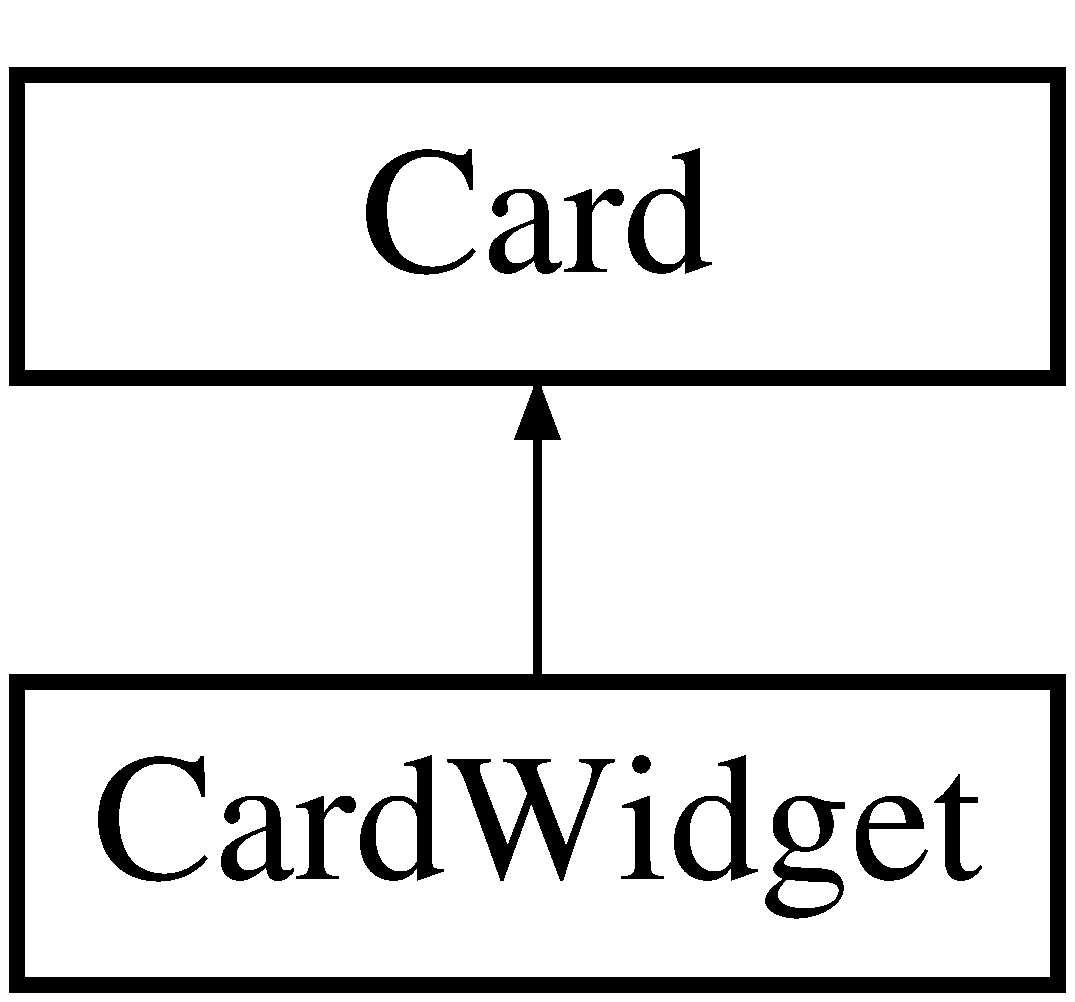
\includegraphics[height=2.000000cm]{class_card}
\end{center}
\end{figure}
\subsection*{Öffentliche Methoden}
\begin{DoxyCompactItemize}
\item 
\hyperlink{class_card_ae26b7b28f4f50dab929144c6cb5cb20a}{Card} (short p\+\_\+color, short p\+\_\+shape, short p\+\_\+number, short p\+\_\+opacity)
\begin{DoxyCompactList}\small\item\em Konstruktor zum Erzeugen einer Card-\/\+Instanz. \end{DoxyCompactList}\item 
\hyperlink{class_card}{Card} \hyperlink{class_card_a4fb042401330d63b6f6695076da4f78f}{operator+} (\hyperlink{class_card}{Card} \&p\+\_\+card)
\begin{DoxyCompactList}\small\item\em Überladener Plus-\/\+Operator, um Karten wie Vektoren zu addieren. \end{DoxyCompactList}\item 
char \hyperlink{class_card_a286395d265732984d23b851b905abb4f}{attributes\+To\+Byte} ()
\begin{DoxyCompactList}\small\item\em Konvertiert alle Attribute zu einem Byte. \end{DoxyCompactList}\item 
\hyperlink{class_card_a097725860cee499e9b99a5d8bb8d4562}{operator char} ()
\begin{DoxyCompactList}\small\item\em Char-\/\+Konvertierungsoperator. \end{DoxyCompactList}\end{DoxyCompactItemize}
\subsection*{Geschützte Attribute}
\begin{DoxyCompactItemize}
\item 
short \hyperlink{class_card_af88f3ff917c623a87d6604d1ec57fe33}{m\+\_\+color}
\begin{DoxyCompactList}\small\item\em Farbe der Karte (Wert im Intervall I = \mbox{[}0;2\mbox{]}) \end{DoxyCompactList}\item 
short \hyperlink{class_card_a4e8799ebd7f3faff5c3998c67c106461}{m\+\_\+shape}
\begin{DoxyCompactList}\small\item\em Form der Karte (Wert im Intervall I = \mbox{[}0;2\mbox{]}) \end{DoxyCompactList}\item 
short \hyperlink{class_card_ac4dc3cf042c39c920dda9ea22b9ef751}{m\+\_\+number}
\begin{DoxyCompactList}\small\item\em Anzahl der Karte (Wert im Intervall I = \mbox{[}0;2\mbox{]}) \end{DoxyCompactList}\item 
short \hyperlink{class_card_a9ad7a67add760db09f496f16a8873ad8}{m\+\_\+opacity}
\begin{DoxyCompactList}\small\item\em Einfärbung der Karte (Wert im Intervall I = \mbox{[}0;2\mbox{]}) \end{DoxyCompactList}\end{DoxyCompactItemize}
\subsection*{Freundbeziehungen}
\begin{DoxyCompactItemize}
\item 
class \hyperlink{class_card_a553f958a25683445088050a69d3de8e9}{Window}
\item 
class \hyperlink{class_card_ac3456fd331a58b288082abca310c7a99}{Controller}
\end{DoxyCompactItemize}


\subsection{Ausführliche Beschreibung}
Die Klasse \hyperlink{class_card}{Card} stellt das digitale pendant zu den analogen Karten des Spiels Set dar. 

\subsection{Beschreibung der Konstruktoren und Destruktoren}
\hypertarget{class_card_ae26b7b28f4f50dab929144c6cb5cb20a}{}\index{Card@{Card}!Card@{Card}}
\index{Card@{Card}!Card@{Card}}
\subsubsection[{Card}]{\setlength{\rightskip}{0pt plus 5cm}Card\+::\+Card (
\begin{DoxyParamCaption}
\item[{short}]{p\+\_\+color, }
\item[{short}]{p\+\_\+shape, }
\item[{short}]{p\+\_\+number, }
\item[{short}]{p\+\_\+opacity}
\end{DoxyParamCaption}
)}\label{class_card_ae26b7b28f4f50dab929144c6cb5cb20a}


Konstruktor zum Erzeugen einer Card-\/\+Instanz. 


\begin{DoxyParams}{Parameter}
{\em p\+\_\+color} & Farbe der zu erzeugenden Karte \\
\hline
{\em p\+\_\+shape} & Form der zu erzeugenden Karte \\
\hline
{\em p\+\_\+number} & Anzahl der zu erzeugenden Karte \\
\hline
{\em p\+\_\+opacity} & Einfärbung der zu erzeugenden Karte \\
\hline
\end{DoxyParams}


\subsection{Dokumentation der Elementfunktionen}
\hypertarget{class_card_a286395d265732984d23b851b905abb4f}{}\index{Card@{Card}!attributes\+To\+Byte@{attributes\+To\+Byte}}
\index{attributes\+To\+Byte@{attributes\+To\+Byte}!Card@{Card}}
\subsubsection[{attributes\+To\+Byte}]{\setlength{\rightskip}{0pt plus 5cm}char Card\+::attributes\+To\+Byte (
\begin{DoxyParamCaption}
{}
\end{DoxyParamCaption}
)}\label{class_card_a286395d265732984d23b851b905abb4f}


Konvertiert alle Attribute zu einem Byte. 

\begin{DoxyReturn}{Rückgabe}
1 Byte, das alle Attribute umfasst 
\end{DoxyReturn}
\hypertarget{class_card_a097725860cee499e9b99a5d8bb8d4562}{}\index{Card@{Card}!operator char@{operator char}}
\index{operator char@{operator char}!Card@{Card}}
\subsubsection[{operator char}]{\setlength{\rightskip}{0pt plus 5cm}Card\+::operator char (
\begin{DoxyParamCaption}
{}
\end{DoxyParamCaption}
)}\label{class_card_a097725860cee499e9b99a5d8bb8d4562}


Char-\/\+Konvertierungsoperator. 

\hypertarget{class_card_a4fb042401330d63b6f6695076da4f78f}{}\index{Card@{Card}!operator+@{operator+}}
\index{operator+@{operator+}!Card@{Card}}
\subsubsection[{operator+}]{\setlength{\rightskip}{0pt plus 5cm}{\bf Card} Card\+::operator+ (
\begin{DoxyParamCaption}
\item[{{\bf Card} \&}]{p\+\_\+card}
\end{DoxyParamCaption}
)}\label{class_card_a4fb042401330d63b6f6695076da4f78f}


Überladener Plus-\/\+Operator, um Karten wie Vektoren zu addieren. 


\begin{DoxyParams}{Parameter}
{\em p\+\_\+card} & Karte die als 2. Summand dient \\
\hline
\end{DoxyParams}
\begin{DoxyReturn}{Rückgabe}
Summe aus der aktuellen Karte und der übergebenen Karte 
\end{DoxyReturn}


\subsection{Freundbeziehungen und Funktionsdokumentation}
\hypertarget{class_card_ac3456fd331a58b288082abca310c7a99}{}\index{Card@{Card}!Controller@{Controller}}
\index{Controller@{Controller}!Card@{Card}}
\subsubsection[{Controller}]{\setlength{\rightskip}{0pt plus 5cm}friend class {\bf Controller}\hspace{0.3cm}{\ttfamily [friend]}}\label{class_card_ac3456fd331a58b288082abca310c7a99}
\hypertarget{class_card_a553f958a25683445088050a69d3de8e9}{}\index{Card@{Card}!Window@{Window}}
\index{Window@{Window}!Card@{Card}}
\subsubsection[{Window}]{\setlength{\rightskip}{0pt plus 5cm}friend class {\bf Window}\hspace{0.3cm}{\ttfamily [friend]}}\label{class_card_a553f958a25683445088050a69d3de8e9}


\subsection{Dokumentation der Datenelemente}
\hypertarget{class_card_af88f3ff917c623a87d6604d1ec57fe33}{}\index{Card@{Card}!m\+\_\+color@{m\+\_\+color}}
\index{m\+\_\+color@{m\+\_\+color}!Card@{Card}}
\subsubsection[{m\+\_\+color}]{\setlength{\rightskip}{0pt plus 5cm}short Card\+::m\+\_\+color\hspace{0.3cm}{\ttfamily [protected]}}\label{class_card_af88f3ff917c623a87d6604d1ec57fe33}


Farbe der Karte (Wert im Intervall I = \mbox{[}0;2\mbox{]}) 

\begin{DoxySeeAlso}{Siehe auch}
\hyperlink{enums_8hpp_ab87bacfdad76e61b9412d7124be44c1c}{Color} 
\end{DoxySeeAlso}
\hypertarget{class_card_ac4dc3cf042c39c920dda9ea22b9ef751}{}\index{Card@{Card}!m\+\_\+number@{m\+\_\+number}}
\index{m\+\_\+number@{m\+\_\+number}!Card@{Card}}
\subsubsection[{m\+\_\+number}]{\setlength{\rightskip}{0pt plus 5cm}short Card\+::m\+\_\+number\hspace{0.3cm}{\ttfamily [protected]}}\label{class_card_ac4dc3cf042c39c920dda9ea22b9ef751}


Anzahl der Karte (Wert im Intervall I = \mbox{[}0;2\mbox{]}) 

\begin{DoxySeeAlso}{Siehe auch}
\hyperlink{enums_8hpp_ad1fb407b73d9c6e54eec2180d3bc4d48}{Number} 
\end{DoxySeeAlso}
\hypertarget{class_card_a9ad7a67add760db09f496f16a8873ad8}{}\index{Card@{Card}!m\+\_\+opacity@{m\+\_\+opacity}}
\index{m\+\_\+opacity@{m\+\_\+opacity}!Card@{Card}}
\subsubsection[{m\+\_\+opacity}]{\setlength{\rightskip}{0pt plus 5cm}short Card\+::m\+\_\+opacity\hspace{0.3cm}{\ttfamily [protected]}}\label{class_card_a9ad7a67add760db09f496f16a8873ad8}


Einfärbung der Karte (Wert im Intervall I = \mbox{[}0;2\mbox{]}) 

\begin{DoxySeeAlso}{Siehe auch}
\hyperlink{enums_8hpp_a31841bed26ecf2fc5a6253eb838aac4b}{Opacity} 
\end{DoxySeeAlso}
\hypertarget{class_card_a4e8799ebd7f3faff5c3998c67c106461}{}\index{Card@{Card}!m\+\_\+shape@{m\+\_\+shape}}
\index{m\+\_\+shape@{m\+\_\+shape}!Card@{Card}}
\subsubsection[{m\+\_\+shape}]{\setlength{\rightskip}{0pt plus 5cm}short Card\+::m\+\_\+shape\hspace{0.3cm}{\ttfamily [protected]}}\label{class_card_a4e8799ebd7f3faff5c3998c67c106461}


Form der Karte (Wert im Intervall I = \mbox{[}0;2\mbox{]}) 

\begin{DoxySeeAlso}{Siehe auch}
\hyperlink{enums_8hpp_a55b506070847a13554f8b879c1bfb37c}{Shape} 
\end{DoxySeeAlso}


Die Dokumentation für diese Klasse wurde erzeugt aufgrund der Dateien\+:\begin{DoxyCompactItemize}
\item 
src/\hyperlink{card_8hpp}{card.\+hpp}\item 
src/\hyperlink{card_8cpp}{card.\+cpp}\end{DoxyCompactItemize}

\hypertarget{class_card_widget}{}\section{Card\+Widget Klassenreferenz}
\label{class_card_widget}\index{Card\+Widget@{Card\+Widget}}


Die grafische Implementierung der Klasse \hyperlink{class_card}{Card}.  




{\ttfamily \#include $<$cardwidget.\+hpp$>$}

Klassendiagramm für Card\+Widget\+:\begin{figure}[H]
\begin{center}
\leavevmode
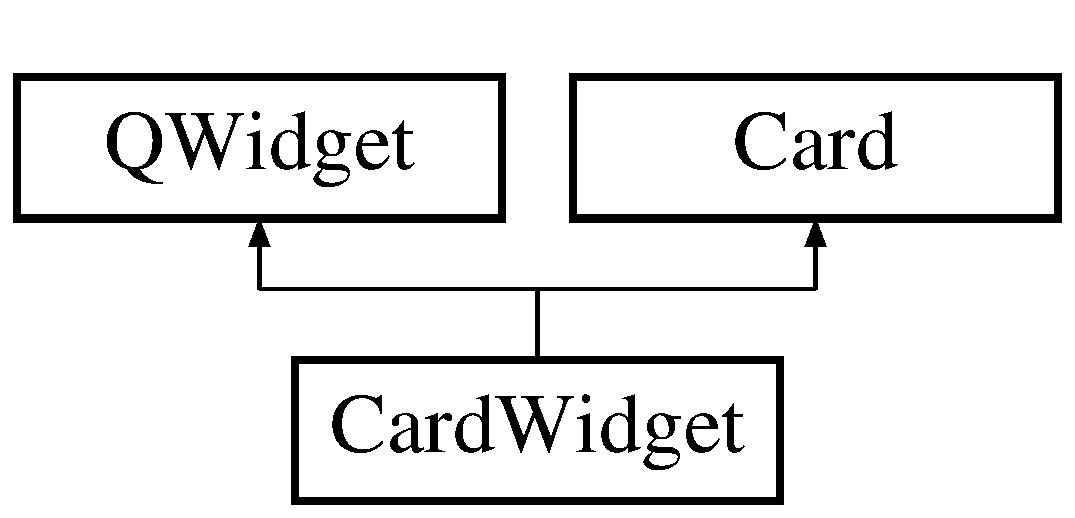
\includegraphics[height=2.000000cm]{class_card_widget}
\end{center}
\end{figure}
\subsection*{Öffentliche Slots}
\begin{DoxyCompactItemize}
\item 
void \hyperlink{class_card_widget_abdf86e7c69cb8d15076a84f61d277797}{unselect} ()
\begin{DoxyCompactList}\small\item\em Wird aufgerufen, wenn eine Karte \char`\"{}entwählt\char`\"{} werden soll. \end{DoxyCompactList}\item 
void \hyperlink{class_card_widget_a67c140043176fa3a911b05d5c11b2115}{can\+Click} (bool p\+\_\+val)
\begin{DoxyCompactList}\small\item\em Wird aufgerufen, um festzulegen, ob man das Card\+Widgets anklicken kann oder eben nicht. \end{DoxyCompactList}\end{DoxyCompactItemize}
\subsection*{Signale}
\begin{DoxyCompactItemize}
\item 
void \hyperlink{class_card_widget_ab3f3a9b457b76a117c218cc1993ee1e4}{clicked} ()
\begin{DoxyCompactList}\small\item\em Signal das emittiert wird, sobald ein Mausklick durchgeführt wird. \end{DoxyCompactList}\end{DoxyCompactItemize}
\subsection*{Öffentliche Methoden}
\begin{DoxyCompactItemize}
\item 
\hyperlink{class_card_widget_a7e385234a42404db9e4d14a9d4241e66}{Card\+Widget} (short p\+\_\+color, short p\+\_\+shape, short p\+\_\+number, short p\+\_\+opacity, Q\+Widget $\ast$parent=0)
\begin{DoxyCompactList}\small\item\em Konstruktor um eine Card\+Widget-\/\+Instanz zu erzeugen. \end{DoxyCompactList}\end{DoxyCompactItemize}
\subsection*{Weitere Geerbte Elemente}


\subsection{Ausführliche Beschreibung}
Die grafische Implementierung der Klasse \hyperlink{class_card}{Card}. 

\begin{DoxySeeAlso}{Siehe auch}
\hyperlink{class_card}{Card} 
\end{DoxySeeAlso}


\subsection{Beschreibung der Konstruktoren und Destruktoren}
\hypertarget{class_card_widget_a7e385234a42404db9e4d14a9d4241e66}{}\index{Card\+Widget@{Card\+Widget}!Card\+Widget@{Card\+Widget}}
\index{Card\+Widget@{Card\+Widget}!Card\+Widget@{Card\+Widget}}
\subsubsection[{Card\+Widget}]{\setlength{\rightskip}{0pt plus 5cm}Card\+Widget\+::\+Card\+Widget (
\begin{DoxyParamCaption}
\item[{short}]{p\+\_\+color, }
\item[{short}]{p\+\_\+shape, }
\item[{short}]{p\+\_\+number, }
\item[{short}]{p\+\_\+opacity, }
\item[{Q\+Widget $\ast$}]{parent = {\ttfamily 0}}
\end{DoxyParamCaption}
)\hspace{0.3cm}{\ttfamily [explicit]}}\label{class_card_widget_a7e385234a42404db9e4d14a9d4241e66}


Konstruktor um eine Card\+Widget-\/\+Instanz zu erzeugen. 


\begin{DoxyParams}{Parameter}
{\em p\+\_\+color} & Farbe des Card\+Wudgets \\
\hline
{\em p\+\_\+shape} & Form des Card\+Widgets \\
\hline
{\em p\+\_\+number} & Anzahl des Card\+Widgets \\
\hline
{\em p\+\_\+opacity} & Einfärbung des Card\+Widgets \\
\hline
{\em parent} & Elternteil des Card\+Widgets \\
\hline
\end{DoxyParams}
\begin{DoxySeeAlso}{Siehe auch}
\hyperlink{enums_8hpp_ab87bacfdad76e61b9412d7124be44c1c}{Color} 

\hyperlink{enums_8hpp_a55b506070847a13554f8b879c1bfb37c}{Shape} 

\hyperlink{enums_8hpp_ad1fb407b73d9c6e54eec2180d3bc4d48}{Number} 

\hyperlink{enums_8hpp_a31841bed26ecf2fc5a6253eb838aac4b}{Opacity} 
\end{DoxySeeAlso}


\subsection{Dokumentation der Elementfunktionen}
\hypertarget{class_card_widget_a67c140043176fa3a911b05d5c11b2115}{}\index{Card\+Widget@{Card\+Widget}!can\+Click@{can\+Click}}
\index{can\+Click@{can\+Click}!Card\+Widget@{Card\+Widget}}
\subsubsection[{can\+Click}]{\setlength{\rightskip}{0pt plus 5cm}void Card\+Widget\+::can\+Click (
\begin{DoxyParamCaption}
\item[{bool}]{p\+\_\+val}
\end{DoxyParamCaption}
)\hspace{0.3cm}{\ttfamily [slot]}}\label{class_card_widget_a67c140043176fa3a911b05d5c11b2115}


Wird aufgerufen, um festzulegen, ob man das Card\+Widgets anklicken kann oder eben nicht. 


\begin{DoxyParams}{Parameter}
{\em p\+\_\+val} & Wahrheitswert der angibt, ob man das Card\+Widgets anklicken kann \\
\hline
\end{DoxyParams}
\hypertarget{class_card_widget_ab3f3a9b457b76a117c218cc1993ee1e4}{}\index{Card\+Widget@{Card\+Widget}!clicked@{clicked}}
\index{clicked@{clicked}!Card\+Widget@{Card\+Widget}}
\subsubsection[{clicked}]{\setlength{\rightskip}{0pt plus 5cm}void Card\+Widget\+::clicked (
\begin{DoxyParamCaption}
{}
\end{DoxyParamCaption}
)\hspace{0.3cm}{\ttfamily [signal]}}\label{class_card_widget_ab3f3a9b457b76a117c218cc1993ee1e4}


Signal das emittiert wird, sobald ein Mausklick durchgeführt wird. 

\hypertarget{class_card_widget_abdf86e7c69cb8d15076a84f61d277797}{}\index{Card\+Widget@{Card\+Widget}!unselect@{unselect}}
\index{unselect@{unselect}!Card\+Widget@{Card\+Widget}}
\subsubsection[{unselect}]{\setlength{\rightskip}{0pt plus 5cm}void Card\+Widget\+::unselect (
\begin{DoxyParamCaption}
{}
\end{DoxyParamCaption}
)\hspace{0.3cm}{\ttfamily [slot]}}\label{class_card_widget_abdf86e7c69cb8d15076a84f61d277797}


Wird aufgerufen, wenn eine Karte \char`\"{}entwählt\char`\"{} werden soll. 



Die Dokumentation für diese Klasse wurde erzeugt aufgrund der Dateien\+:\begin{DoxyCompactItemize}
\item 
src/\hyperlink{cardwidget_8hpp}{cardwidget.\+hpp}\item 
src/\hyperlink{cardwidget_8cpp}{cardwidget.\+cpp}\end{DoxyCompactItemize}

\hypertarget{class_client}{}\section{Client Klassenreferenz}
\label{class_client}\index{Client@{Client}}


Die abstrakte Klasse \hyperlink{class_client}{Client} kümmert sich um die Verbindung zum \hyperlink{class_server}{Server} und macht so ein Spielen möglich.  




{\ttfamily \#include $<$client.\+hpp$>$}

Klassendiagramm für Client\+:\begin{figure}[H]
\begin{center}
\leavevmode
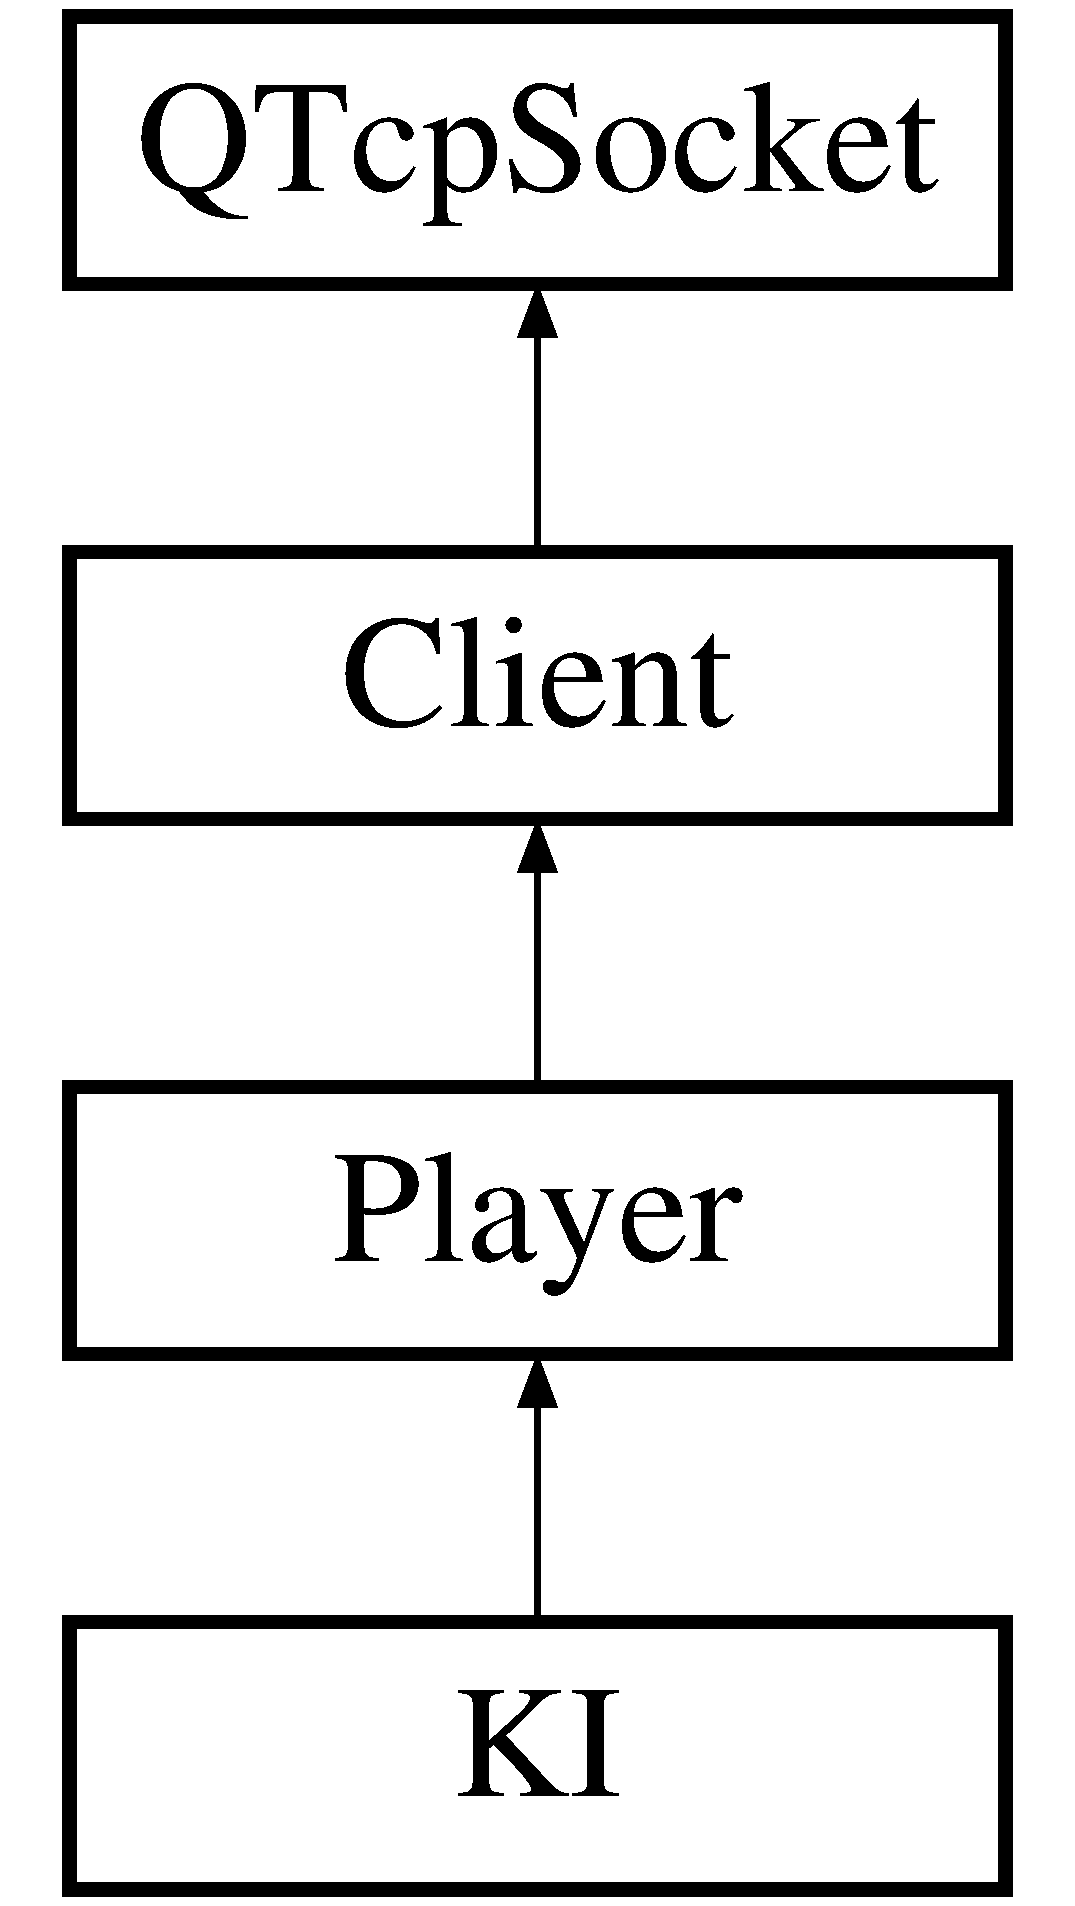
\includegraphics[height=4.000000cm]{class_client}
\end{center}
\end{figure}
\subsection*{Öffentliche Slots}
\begin{DoxyCompactItemize}
\item 
void \hyperlink{class_client_a1e1df136ba1989a25261aed93a46c6a1}{on\+Ready\+Read} ()
\begin{DoxyCompactList}\small\item\em Wird aufgerufen, sobald der Buffer mit den eingehenden Paketen lesebereit ist. \end{DoxyCompactList}\end{DoxyCompactItemize}
\subsection*{Öffentliche Methoden}
\begin{DoxyCompactItemize}
\item 
\hyperlink{class_client_ade80139efef3b5a858968ccf20563709}{Client} (Q\+Object $\ast$p\+\_\+parent=0, Q\+Host\+Address p\+\_\+ip=Q\+Host\+Address\+::\+Local\+Host, int p\+\_\+port=1337)
\begin{DoxyCompactList}\small\item\em Konstruktor zum Erzeugen einer Client-\/\+Instanz. \end{DoxyCompactList}\item 
virtual void \hyperlink{class_client_ac3b60506d2f900a3490a05425f392914}{send\+Click\+Packet} (Q\+Byte\+Array p\+\_\+cards)=0
\begin{DoxyCompactList}\small\item\em Sendet ein Klick-\/\+Paket -\/ mit den ausgewählten Karten -\/ an den \hyperlink{class_server}{Server}.~\newline
 (Muss von Klasse \hyperlink{class_player}{Player} definiert werden) \end{DoxyCompactList}\item 
virtual void \hyperlink{class_client_a62fc6262c8e9f0e9a0b2811a9c6fa8b0}{send\+Turn\+Packet} ()=0
\begin{DoxyCompactList}\small\item\em Sendet ein Paket an den \hyperlink{class_server}{Server} das angibt, dass der aktuelle Socket am Zug ist.~\newline
 (Muss von Klasse \hyperlink{class_player}{Player} definiert werden) \end{DoxyCompactList}\end{DoxyCompactItemize}
\subsection*{Geschützte Attribute}
\begin{DoxyCompactItemize}
\item 
\hyperlink{class_packet_handler}{Packet\+Handler} $\ast$ \hyperlink{class_client_a4f9222fa01234b1ebdbe909f13e15744}{m\+\_\+packet\+Handler}
\begin{DoxyCompactList}\small\item\em Paketverwalter für ein-\/ und ausgehende Pakete. \end{DoxyCompactList}\end{DoxyCompactItemize}


\subsection{Ausführliche Beschreibung}
Die abstrakte Klasse \hyperlink{class_client}{Client} kümmert sich um die Verbindung zum \hyperlink{class_server}{Server} und macht so ein Spielen möglich. 

\subsection{Beschreibung der Konstruktoren und Destruktoren}
\hypertarget{class_client_ade80139efef3b5a858968ccf20563709}{}\index{Client@{Client}!Client@{Client}}
\index{Client@{Client}!Client@{Client}}
\subsubsection[{Client}]{\setlength{\rightskip}{0pt plus 5cm}Client\+::\+Client (
\begin{DoxyParamCaption}
\item[{Q\+Object $\ast$}]{p\+\_\+parent = {\ttfamily 0}, }
\item[{Q\+Host\+Address}]{p\+\_\+ip = {\ttfamily QHostAddress\+:\+:LocalHost}, }
\item[{int}]{p\+\_\+port = {\ttfamily 1337}}
\end{DoxyParamCaption}
)\hspace{0.3cm}{\ttfamily [explicit]}}\label{class_client_ade80139efef3b5a858968ccf20563709}


Konstruktor zum Erzeugen einer Client-\/\+Instanz. 


\begin{DoxyParams}{Parameter}
{\em p\+\_\+parent} & Elternteil des Clients \\
\hline
{\em p\+\_\+ip} & I\+P-\/\+Adresse mit der sich der \hyperlink{class_client}{Client} verbinden soll \\
\hline
{\em p\+\_\+port} & Port, auf dem die Verbindung stattfindet \\
\hline
\end{DoxyParams}


\subsection{Dokumentation der Elementfunktionen}
\hypertarget{class_client_a1e1df136ba1989a25261aed93a46c6a1}{}\index{Client@{Client}!on\+Ready\+Read@{on\+Ready\+Read}}
\index{on\+Ready\+Read@{on\+Ready\+Read}!Client@{Client}}
\subsubsection[{on\+Ready\+Read}]{\setlength{\rightskip}{0pt plus 5cm}void Client\+::on\+Ready\+Read (
\begin{DoxyParamCaption}
{}
\end{DoxyParamCaption}
)\hspace{0.3cm}{\ttfamily [slot]}}\label{class_client_a1e1df136ba1989a25261aed93a46c6a1}


Wird aufgerufen, sobald der Buffer mit den eingehenden Paketen lesebereit ist. 

\hypertarget{class_client_ac3b60506d2f900a3490a05425f392914}{}\index{Client@{Client}!send\+Click\+Packet@{send\+Click\+Packet}}
\index{send\+Click\+Packet@{send\+Click\+Packet}!Client@{Client}}
\subsubsection[{send\+Click\+Packet}]{\setlength{\rightskip}{0pt plus 5cm}virtual void Client\+::send\+Click\+Packet (
\begin{DoxyParamCaption}
\item[{Q\+Byte\+Array}]{p\+\_\+cards}
\end{DoxyParamCaption}
)\hspace{0.3cm}{\ttfamily [pure virtual]}}\label{class_client_ac3b60506d2f900a3490a05425f392914}


Sendet ein Klick-\/\+Paket -\/ mit den ausgewählten Karten -\/ an den \hyperlink{class_server}{Server}.~\newline
 (Muss von Klasse \hyperlink{class_player}{Player} definiert werden) 


\begin{DoxyParams}{Parameter}
{\em p\+\_\+cards} & Array bestehend aus den angewählten Karten \\
\hline
\end{DoxyParams}


Implementiert in \hyperlink{class_player_ae688e0cb60be7901e195d7881b4d39ce}{Player}.

\hypertarget{class_client_a62fc6262c8e9f0e9a0b2811a9c6fa8b0}{}\index{Client@{Client}!send\+Turn\+Packet@{send\+Turn\+Packet}}
\index{send\+Turn\+Packet@{send\+Turn\+Packet}!Client@{Client}}
\subsubsection[{send\+Turn\+Packet}]{\setlength{\rightskip}{0pt plus 5cm}virtual void Client\+::send\+Turn\+Packet (
\begin{DoxyParamCaption}
{}
\end{DoxyParamCaption}
)\hspace{0.3cm}{\ttfamily [pure virtual]}}\label{class_client_a62fc6262c8e9f0e9a0b2811a9c6fa8b0}


Sendet ein Paket an den \hyperlink{class_server}{Server} das angibt, dass der aktuelle Socket am Zug ist.~\newline
 (Muss von Klasse \hyperlink{class_player}{Player} definiert werden) 



Implementiert in \hyperlink{class_player_a08220f4cd6aa057071371a7c815a63dd}{Player}.



\subsection{Dokumentation der Datenelemente}
\hypertarget{class_client_a4f9222fa01234b1ebdbe909f13e15744}{}\index{Client@{Client}!m\+\_\+packet\+Handler@{m\+\_\+packet\+Handler}}
\index{m\+\_\+packet\+Handler@{m\+\_\+packet\+Handler}!Client@{Client}}
\subsubsection[{m\+\_\+packet\+Handler}]{\setlength{\rightskip}{0pt plus 5cm}{\bf Packet\+Handler}$\ast$ Client\+::m\+\_\+packet\+Handler\hspace{0.3cm}{\ttfamily [protected]}}\label{class_client_a4f9222fa01234b1ebdbe909f13e15744}


Paketverwalter für ein-\/ und ausgehende Pakete. 

\begin{DoxySeeAlso}{Siehe auch}
\hyperlink{class_packet_handler}{Packet\+Handler} 
\end{DoxySeeAlso}


Die Dokumentation für diese Klasse wurde erzeugt aufgrund der Dateien\+:\begin{DoxyCompactItemize}
\item 
src/\hyperlink{client_8hpp}{client.\+hpp}\item 
src/\hyperlink{client_8cpp}{client.\+cpp}\end{DoxyCompactItemize}

\hypertarget{class_controller}{}\section{Controller Klassenreferenz}
\label{class_controller}\index{Controller@{Controller}}


Die Klasse \hyperlink{class_controller}{Controller} ist für den kompletten Spielverlauf zuständig.~\newline
 Sie regelt, wann welcher \hyperlink{class_client}{Client} welche Pakete empfängt, wann das Spiel zu Ende ist/anfängt und~\newline
 wenn Karten nachgelegt werden sollen.  




{\ttfamily \#include $<$controller.\+hpp$>$}

Klassendiagramm für Controller\+:\begin{figure}[H]
\begin{center}
\leavevmode
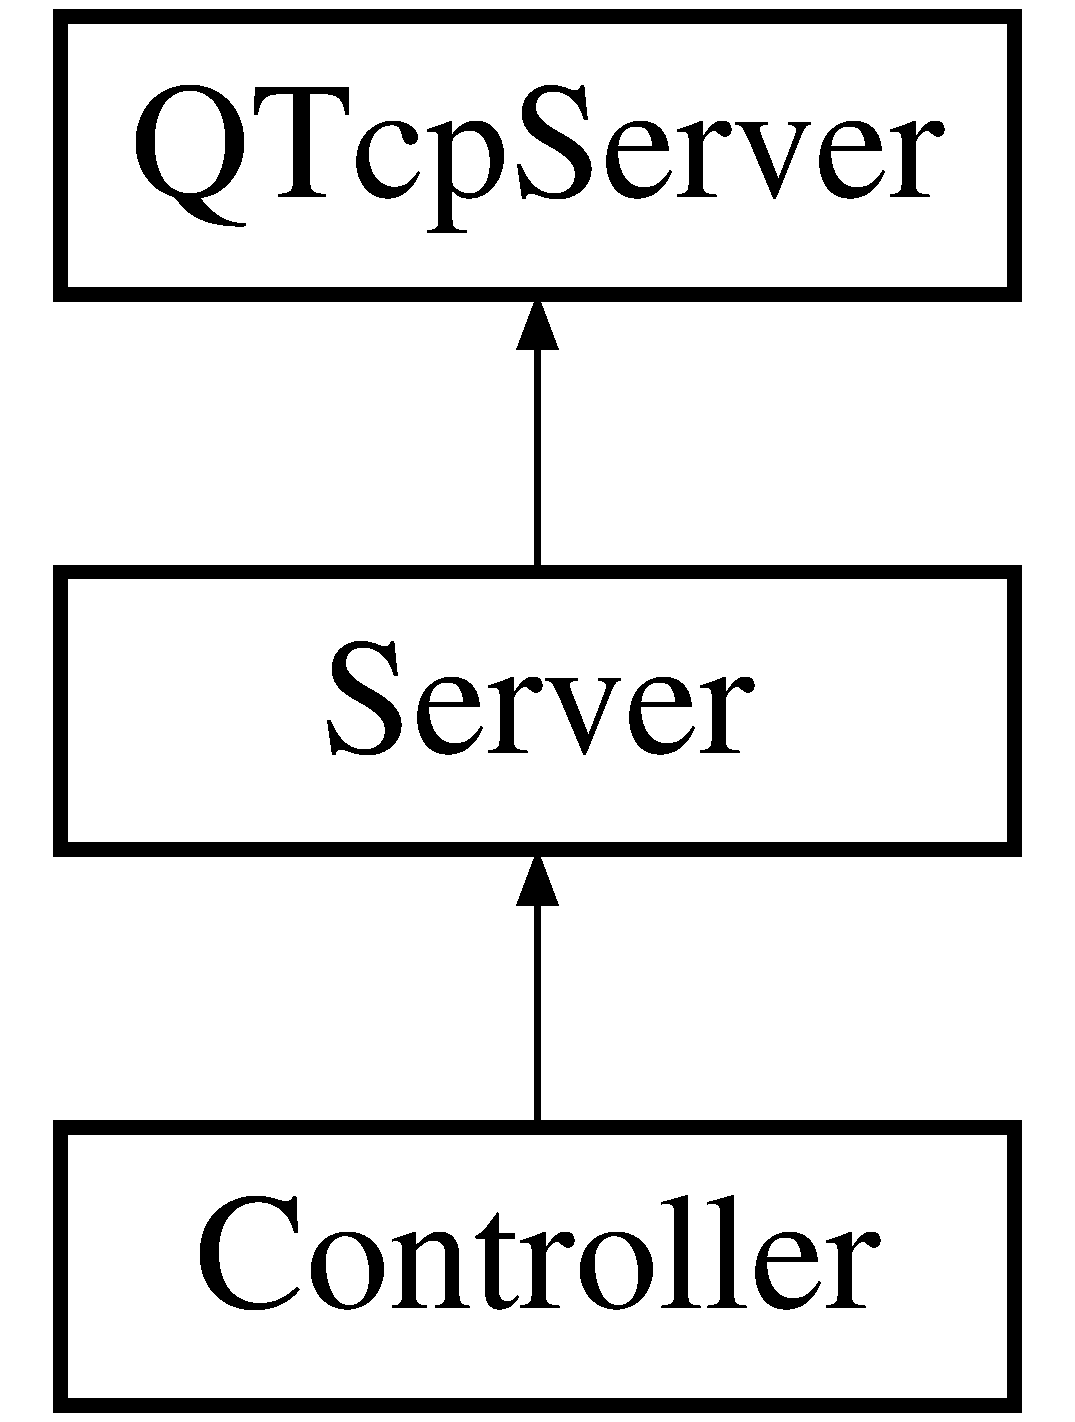
\includegraphics[height=3.000000cm]{class_controller}
\end{center}
\end{figure}
\subsection*{Öffentliche Slots}
\begin{DoxyCompactItemize}
\item 
void \hyperlink{class_controller_ad54697994dab06b6340cd674af53f7e2}{draw} (unsigned int p\+\_\+count=3)
\begin{DoxyCompactList}\small\item\em Zieht eine bestimmte Anzahl zufälliger Karten aus dem Deck und legt sie aufs Spielfeld.~\newline
 Danach wird eine Spielfeld-\/\+Synchronisation ausgeführt. \end{DoxyCompactList}\item 
void \hyperlink{class_controller_a0283cf55f555625b3df2cb0b3557d61b}{retrieve\+Click} (Q\+Tcp\+Socket $\ast$p\+\_\+client, Q\+Byte\+Array p\+\_\+cards)
\begin{DoxyCompactList}\small\item\em Wird aufgerufen, wenn ein Set ausgewählt wurde.~\newline
 Das Set wird überprüft und dementsprechend Punkte gutgeschrieben oder abgezogen. \end{DoxyCompactList}\item 
void \hyperlink{class_controller_a74bfe4153a8b5d66621bb19c76767d8c}{retrieve\+Player\+Turn} (Q\+Tcp\+Socket $\ast$p\+\_\+socket)
\begin{DoxyCompactList}\small\item\em Wird aufgerufen, sobald ein Spieler ein Set auswählen möchte. \end{DoxyCompactList}\end{DoxyCompactItemize}
\subsection*{Signale}
\begin{DoxyCompactItemize}
\item 
void \hyperlink{class_controller_a7b451f4eb09398e825910d02e73f8789}{show\+Start\+Button} ()
\begin{DoxyCompactList}\small\item\em Wird emittiert, um den Startbutton auf dem Hauptfenster anzuzeigen. \end{DoxyCompactList}\end{DoxyCompactItemize}
\subsection*{Öffentliche Methoden}
\begin{DoxyCompactItemize}
\item 
void \hyperlink{class_controller_a07ee1874817ee0abd630e846e7b37ea9}{send\+Game\+Started\+Packet} ()
\begin{DoxyCompactList}\small\item\em Sendet das Paket, um das Spiel zu starten. \end{DoxyCompactList}\item 
\hyperlink{class_controller_aa3d04afa037846c8eea68ccb37159760}{Controller} (Q\+Object $\ast$p\+\_\+parent=0)
\begin{DoxyCompactList}\small\item\em Konstruktor zum Erzeugen einer Controller-\/\+Instanz. \end{DoxyCompactList}\end{DoxyCompactItemize}
\subsection*{Öffentliche, statische Methoden}
\begin{DoxyCompactItemize}
\item 
static bool \hyperlink{class_controller_a631b306cacf6c59b6185152f8ea25fa3}{check} (\hyperlink{class_server_a2b2ff2c4678bdca3599c3feb5efdaff7}{Cards} \&p\+\_\+cards)
\begin{DoxyCompactList}\small\item\em Überprüft ob eine Liste aus Karten ein Set bilden. \end{DoxyCompactList}\end{DoxyCompactItemize}
\subsection*{Weitere Geerbte Elemente}


\subsection{Ausführliche Beschreibung}
Die Klasse \hyperlink{class_controller}{Controller} ist für den kompletten Spielverlauf zuständig.~\newline
 Sie regelt, wann welcher \hyperlink{class_client}{Client} welche Pakete empfängt, wann das Spiel zu Ende ist/anfängt und~\newline
 wenn Karten nachgelegt werden sollen. 

\subsection{Beschreibung der Konstruktoren und Destruktoren}
\hypertarget{class_controller_aa3d04afa037846c8eea68ccb37159760}{}\index{Controller@{Controller}!Controller@{Controller}}
\index{Controller@{Controller}!Controller@{Controller}}
\subsubsection[{Controller}]{\setlength{\rightskip}{0pt plus 5cm}Controller\+::\+Controller (
\begin{DoxyParamCaption}
\item[{Q\+Object $\ast$}]{p\+\_\+parent = {\ttfamily 0}}
\end{DoxyParamCaption}
)}\label{class_controller_aa3d04afa037846c8eea68ccb37159760}


Konstruktor zum Erzeugen einer Controller-\/\+Instanz. 


\begin{DoxyParams}{Parameter}
{\em p\+\_\+parent} & Elternteil des Controllers \\
\hline
\end{DoxyParams}


\subsection{Dokumentation der Elementfunktionen}
\hypertarget{class_controller_a631b306cacf6c59b6185152f8ea25fa3}{}\index{Controller@{Controller}!check@{check}}
\index{check@{check}!Controller@{Controller}}
\subsubsection[{check}]{\setlength{\rightskip}{0pt plus 5cm}bool Controller\+::check (
\begin{DoxyParamCaption}
\item[{{\bf Server\+::\+Cards} \&}]{p\+\_\+cards}
\end{DoxyParamCaption}
)\hspace{0.3cm}{\ttfamily [static]}}\label{class_controller_a631b306cacf6c59b6185152f8ea25fa3}


Überprüft ob eine Liste aus Karten ein Set bilden. 


\begin{DoxyParams}{Parameter}
{\em p\+\_\+cards} & Liste aus zu überprüfenden Karten \\
\hline
\end{DoxyParams}
\begin{DoxyReturn}{Rückgabe}
Wahrheitswert der angibt, ob die Karten ein Set bilden 
\end{DoxyReturn}
\hypertarget{class_controller_ad54697994dab06b6340cd674af53f7e2}{}\index{Controller@{Controller}!draw@{draw}}
\index{draw@{draw}!Controller@{Controller}}
\subsubsection[{draw}]{\setlength{\rightskip}{0pt plus 5cm}void Controller\+::draw (
\begin{DoxyParamCaption}
\item[{unsigned int}]{p\+\_\+count = {\ttfamily 3}}
\end{DoxyParamCaption}
)\hspace{0.3cm}{\ttfamily [slot]}}\label{class_controller_ad54697994dab06b6340cd674af53f7e2}


Zieht eine bestimmte Anzahl zufälliger Karten aus dem Deck und legt sie aufs Spielfeld.~\newline
 Danach wird eine Spielfeld-\/\+Synchronisation ausgeführt. 


\begin{DoxyParams}{Parameter}
{\em p\+\_\+count} & \\
\hline
\end{DoxyParams}
\hypertarget{class_controller_a0283cf55f555625b3df2cb0b3557d61b}{}\index{Controller@{Controller}!retrieve\+Click@{retrieve\+Click}}
\index{retrieve\+Click@{retrieve\+Click}!Controller@{Controller}}
\subsubsection[{retrieve\+Click}]{\setlength{\rightskip}{0pt plus 5cm}void Controller\+::retrieve\+Click (
\begin{DoxyParamCaption}
\item[{Q\+Tcp\+Socket $\ast$}]{p\+\_\+client, }
\item[{Q\+Byte\+Array}]{p\+\_\+cards}
\end{DoxyParamCaption}
)\hspace{0.3cm}{\ttfamily [slot]}}\label{class_controller_a0283cf55f555625b3df2cb0b3557d61b}


Wird aufgerufen, wenn ein Set ausgewählt wurde.~\newline
 Das Set wird überprüft und dementsprechend Punkte gutgeschrieben oder abgezogen. 


\begin{DoxyParams}{Parameter}
{\em p\+\_\+client} & Spieler, der das Set ausgewählt hat \\
\hline
{\em p\+\_\+cards} & Die ausgewählten Karten \\
\hline
\end{DoxyParams}
\begin{DoxySeeAlso}{Siehe auch}
\hyperlink{class_packet_handler_a8cb91da2e7e174f5b781d5338a54427e}{Packet\+Handler\+::read\+Click} 
\end{DoxySeeAlso}
\hypertarget{class_controller_a74bfe4153a8b5d66621bb19c76767d8c}{}\index{Controller@{Controller}!retrieve\+Player\+Turn@{retrieve\+Player\+Turn}}
\index{retrieve\+Player\+Turn@{retrieve\+Player\+Turn}!Controller@{Controller}}
\subsubsection[{retrieve\+Player\+Turn}]{\setlength{\rightskip}{0pt plus 5cm}void Controller\+::retrieve\+Player\+Turn (
\begin{DoxyParamCaption}
\item[{Q\+Tcp\+Socket $\ast$}]{p\+\_\+socket}
\end{DoxyParamCaption}
)\hspace{0.3cm}{\ttfamily [slot]}}\label{class_controller_a74bfe4153a8b5d66621bb19c76767d8c}


Wird aufgerufen, sobald ein Spieler ein Set auswählen möchte. 


\begin{DoxyParams}{Parameter}
{\em p\+\_\+socket} & \hyperlink{class_client}{Client}, dem das Anklicken der Karten gewährt ist \\
\hline
\end{DoxyParams}
\begin{DoxySeeAlso}{Siehe auch}
\hyperlink{class_packet_handler_aceaa87f977376e769e840db3e0756bfe}{Packet\+Handler\+::read\+Turn\+Packet} 
\end{DoxySeeAlso}
\hypertarget{class_controller_a07ee1874817ee0abd630e846e7b37ea9}{}\index{Controller@{Controller}!send\+Game\+Started\+Packet@{send\+Game\+Started\+Packet}}
\index{send\+Game\+Started\+Packet@{send\+Game\+Started\+Packet}!Controller@{Controller}}
\subsubsection[{send\+Game\+Started\+Packet}]{\setlength{\rightskip}{0pt plus 5cm}void Controller\+::send\+Game\+Started\+Packet (
\begin{DoxyParamCaption}
{}
\end{DoxyParamCaption}
)\hspace{0.3cm}{\ttfamily [virtual]}}\label{class_controller_a07ee1874817ee0abd630e846e7b37ea9}


Sendet das Paket, um das Spiel zu starten. 

\begin{DoxySeeAlso}{Siehe auch}
\hyperlink{class_packet_handler_aef3b383774fb1894dcd99dd40b3f735a}{Packet\+Handler\+::make\+Game\+Started\+Packet} 
\end{DoxySeeAlso}


Implementiert \hyperlink{class_server_a1be346a3252468e445f8f809d1c912e7}{Server}.

\hypertarget{class_controller_a7b451f4eb09398e825910d02e73f8789}{}\index{Controller@{Controller}!show\+Start\+Button@{show\+Start\+Button}}
\index{show\+Start\+Button@{show\+Start\+Button}!Controller@{Controller}}
\subsubsection[{show\+Start\+Button}]{\setlength{\rightskip}{0pt plus 5cm}void Controller\+::show\+Start\+Button (
\begin{DoxyParamCaption}
{}
\end{DoxyParamCaption}
)\hspace{0.3cm}{\ttfamily [signal]}}\label{class_controller_a7b451f4eb09398e825910d02e73f8789}


Wird emittiert, um den Startbutton auf dem Hauptfenster anzuzeigen. 

\begin{DoxySeeAlso}{Siehe auch}
\hyperlink{class_window_ab182caf7adf8a0227b8758cc37127b10}{Window\+::retrieve\+Show\+Start\+Button} 
\end{DoxySeeAlso}


Die Dokumentation für diese Klasse wurde erzeugt aufgrund der Dateien\+:\begin{DoxyCompactItemize}
\item 
src/\hyperlink{controller_8hpp}{controller.\+hpp}\item 
src/\hyperlink{controller_8cpp}{controller.\+cpp}\end{DoxyCompactItemize}

\hypertarget{class_information_widget}{}\section{Information\+Widget Klassenreferenz}
\label{class_information_widget}\index{Information\+Widget@{Information\+Widget}}


Das \hyperlink{class_information_widget}{Information\+Widget} dient zur Ausgabe des Spielstatuses.  




{\ttfamily \#include $<$informationwidget.\+hpp$>$}

Klassendiagramm für Information\+Widget\+:\begin{figure}[H]
\begin{center}
\leavevmode
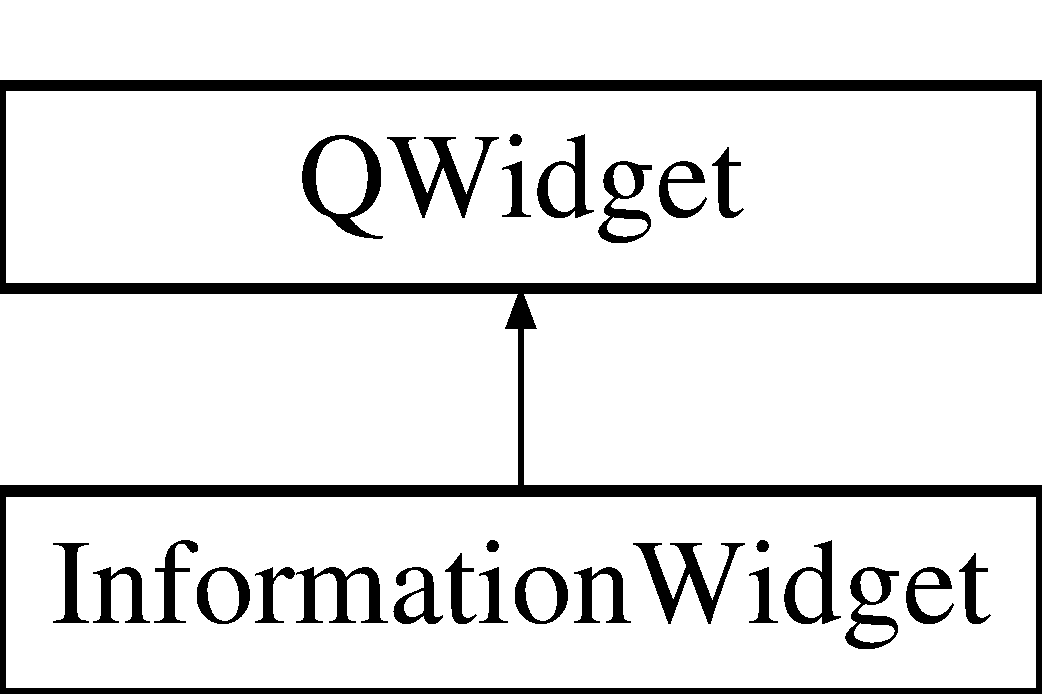
\includegraphics[height=2.000000cm]{class_information_widget}
\end{center}
\end{figure}
\subsection*{Öffentliche Methoden}
\begin{DoxyCompactItemize}
\item 
\hyperlink{class_information_widget_aabe49df48595f6e13addb6619105359a}{Information\+Widget} (Q\+Widget $\ast$parent=0)
\begin{DoxyCompactList}\small\item\em Konstruktor zum Erzeugen einer Information\+Widget-\/\+Instanz. \end{DoxyCompactList}\item 
void \hyperlink{class_information_widget_a07210421d5e1283806416489736a1c85}{set\+Player\+Count} (short p\+\_\+player\+Count)
\begin{DoxyCompactList}\small\item\em Legt die Anzahl der Spieler fest. \end{DoxyCompactList}\item 
void \hyperlink{class_information_widget_aca27b73fb7bf5e772327141b0f83d08d}{set\+Deck\+Length} (short p\+\_\+deck\+Length)
\begin{DoxyCompactList}\small\item\em Legt die Anzahl der Karten im Deck fest. \end{DoxyCompactList}\item 
void \hyperlink{class_information_widget_ac79ef86fb429a6179cb90932d2ea8766}{set\+Scores} (Q\+Byte\+Array p\+\_\+scores)
\begin{DoxyCompactList}\small\item\em Legt den Inhalt des Scoreboards fest. \end{DoxyCompactList}\end{DoxyCompactItemize}


\subsection{Ausführliche Beschreibung}
Das \hyperlink{class_information_widget}{Information\+Widget} dient zur Ausgabe des Spielstatuses. 

\subsection{Beschreibung der Konstruktoren und Destruktoren}
\hypertarget{class_information_widget_aabe49df48595f6e13addb6619105359a}{}\index{Information\+Widget@{Information\+Widget}!Information\+Widget@{Information\+Widget}}
\index{Information\+Widget@{Information\+Widget}!Information\+Widget@{Information\+Widget}}
\subsubsection[{Information\+Widget}]{\setlength{\rightskip}{0pt plus 5cm}Information\+Widget\+::\+Information\+Widget (
\begin{DoxyParamCaption}
\item[{Q\+Widget $\ast$}]{parent = {\ttfamily 0}}
\end{DoxyParamCaption}
)\hspace{0.3cm}{\ttfamily [explicit]}}\label{class_information_widget_aabe49df48595f6e13addb6619105359a}


Konstruktor zum Erzeugen einer Information\+Widget-\/\+Instanz. 


\begin{DoxyParams}{Parameter}
{\em parent} & Elternteil des Information\+Widgets \\
\hline
\end{DoxyParams}


\subsection{Dokumentation der Elementfunktionen}
\hypertarget{class_information_widget_aca27b73fb7bf5e772327141b0f83d08d}{}\index{Information\+Widget@{Information\+Widget}!set\+Deck\+Length@{set\+Deck\+Length}}
\index{set\+Deck\+Length@{set\+Deck\+Length}!Information\+Widget@{Information\+Widget}}
\subsubsection[{set\+Deck\+Length}]{\setlength{\rightskip}{0pt plus 5cm}void Information\+Widget\+::set\+Deck\+Length (
\begin{DoxyParamCaption}
\item[{short}]{p\+\_\+deck\+Length}
\end{DoxyParamCaption}
)}\label{class_information_widget_aca27b73fb7bf5e772327141b0f83d08d}


Legt die Anzahl der Karten im Deck fest. 


\begin{DoxyParams}{Parameter}
{\em p\+\_\+deck\+Length} & Anzahl der Karten im Deck \\
\hline
\end{DoxyParams}
\begin{DoxySeeAlso}{Siehe auch}
m\+\_\+deck\+Length 
\end{DoxySeeAlso}
\hypertarget{class_information_widget_a07210421d5e1283806416489736a1c85}{}\index{Information\+Widget@{Information\+Widget}!set\+Player\+Count@{set\+Player\+Count}}
\index{set\+Player\+Count@{set\+Player\+Count}!Information\+Widget@{Information\+Widget}}
\subsubsection[{set\+Player\+Count}]{\setlength{\rightskip}{0pt plus 5cm}void Information\+Widget\+::set\+Player\+Count (
\begin{DoxyParamCaption}
\item[{short}]{p\+\_\+player\+Count}
\end{DoxyParamCaption}
)}\label{class_information_widget_a07210421d5e1283806416489736a1c85}


Legt die Anzahl der Spieler fest. 


\begin{DoxyParams}{Parameter}
{\em p\+\_\+player\+Count} & Spieleranzahl \\
\hline
\end{DoxyParams}
\begin{DoxySeeAlso}{Siehe auch}
m\+\_\+player\+Count 
\end{DoxySeeAlso}
\hypertarget{class_information_widget_ac79ef86fb429a6179cb90932d2ea8766}{}\index{Information\+Widget@{Information\+Widget}!set\+Scores@{set\+Scores}}
\index{set\+Scores@{set\+Scores}!Information\+Widget@{Information\+Widget}}
\subsubsection[{set\+Scores}]{\setlength{\rightskip}{0pt plus 5cm}void Information\+Widget\+::set\+Scores (
\begin{DoxyParamCaption}
\item[{Q\+Byte\+Array}]{p\+\_\+scores}
\end{DoxyParamCaption}
)}\label{class_information_widget_ac79ef86fb429a6179cb90932d2ea8766}


Legt den Inhalt des Scoreboards fest. 


\begin{DoxyParams}{Parameter}
{\em p\+\_\+scores} & Punktestand \\
\hline
\end{DoxyParams}
\begin{DoxySeeAlso}{Siehe auch}
m\+\_\+scores 
\end{DoxySeeAlso}


Die Dokumentation für diese Klasse wurde erzeugt aufgrund der Dateien\+:\begin{DoxyCompactItemize}
\item 
src/\hyperlink{informationwidget_8hpp}{informationwidget.\+hpp}\item 
src/\hyperlink{informationwidget_8cpp}{informationwidget.\+cpp}\end{DoxyCompactItemize}

\hypertarget{class_k_i}{}\section{K\+I Klassenreferenz}
\label{class_k_i}\index{K\+I@{K\+I}}


{\ttfamily \#include $<$ki.\+hpp$>$}

Klassendiagramm für K\+I\+:\begin{figure}[H]
\begin{center}
\leavevmode
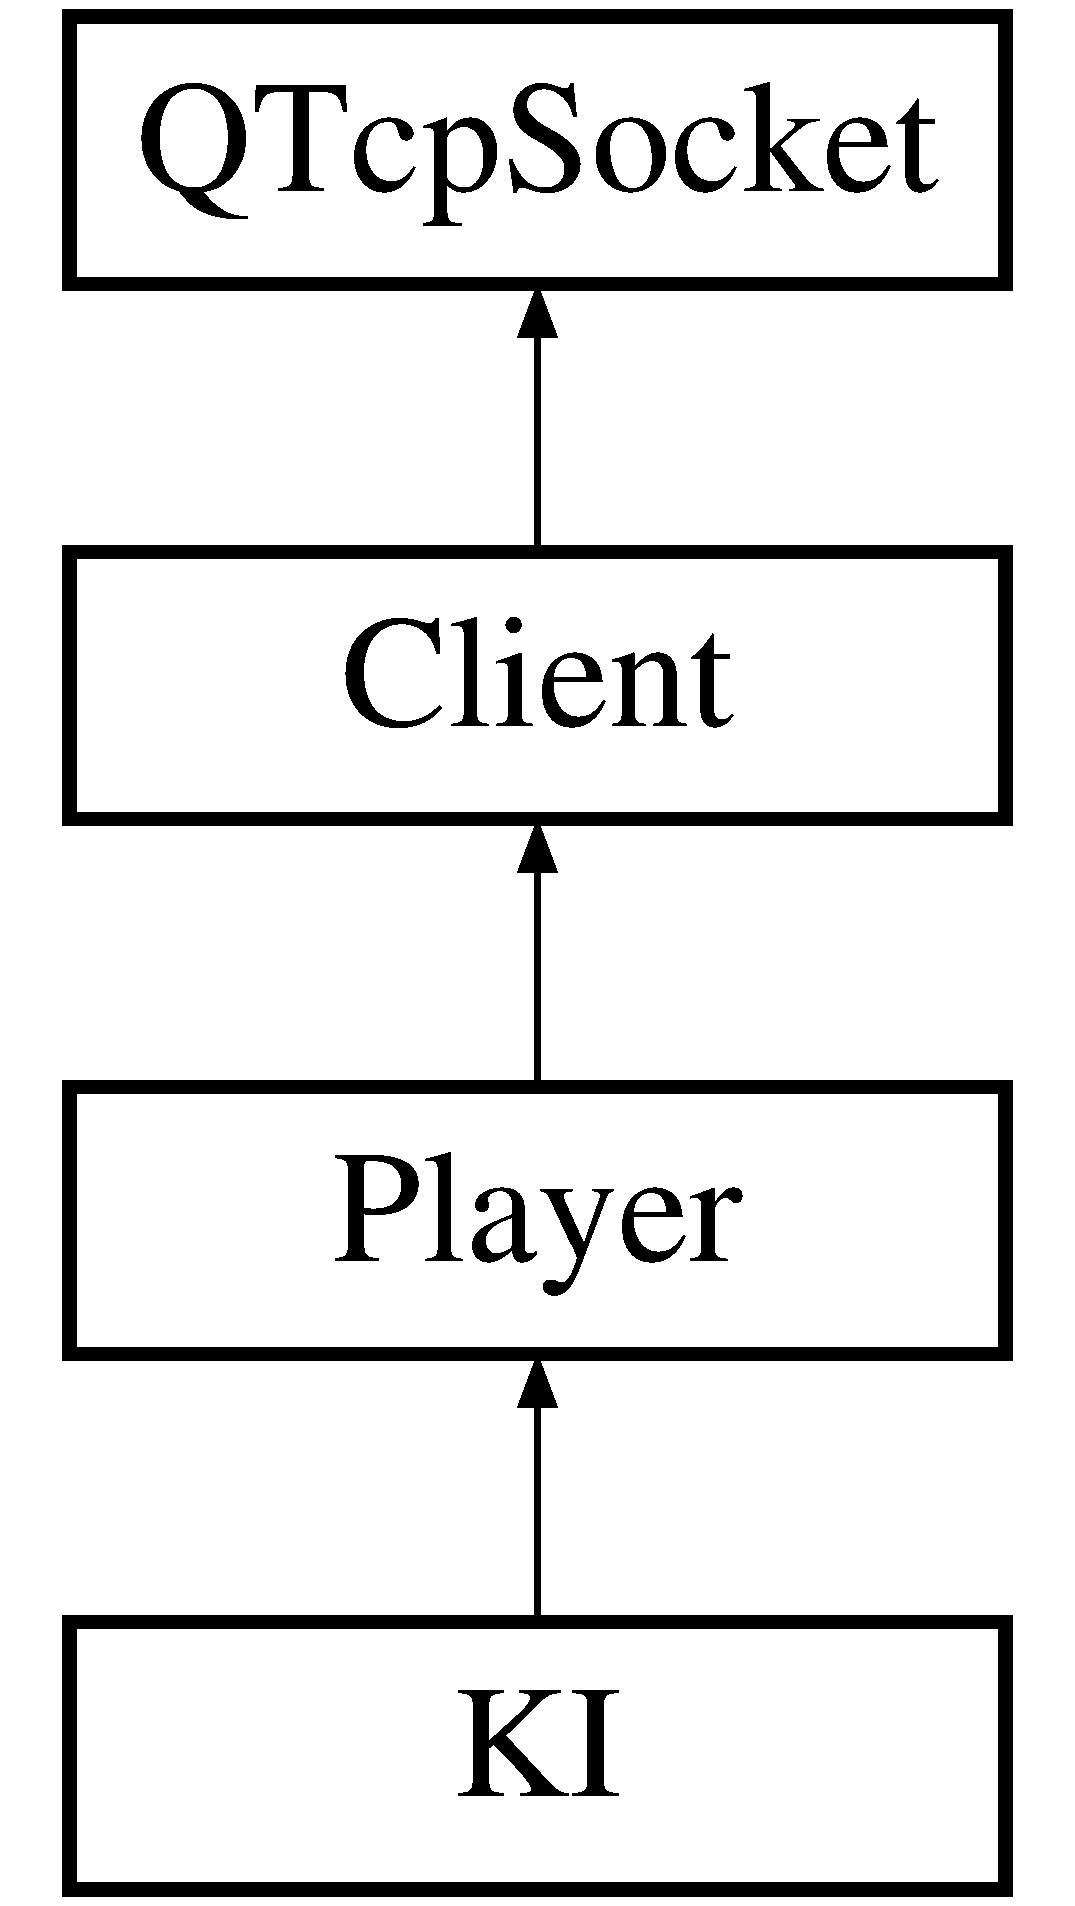
\includegraphics[height=4.000000cm]{class_k_i}
\end{center}
\end{figure}
\subsection*{Öffentliche Slots}
\begin{DoxyCompactItemize}
\item 
void \hyperlink{class_k_i_a1c69c3c3ef246e360bc5fc20823e4223}{retrieve\+Input\+Unlocked} ()
\item 
void \hyperlink{class_k_i_a1f807b37c8d3f39f05c7681bf64712e7}{retrieve\+Input\+Locked} ()
\item 
void \hyperlink{class_k_i_ace9a8c3acb7f18dc16ad5bf69323d558}{retrieve\+Game\+Started} ()
\item 
void \hyperlink{class_k_i_a16aea3f051dd748d5f5760bba3c4a2a5}{retrieve\+Game\+Ended} ()
\item 
void \hyperlink{class_k_i_a6c6fa186116552a3c56fb50b17c108a7}{retrieve\+Field} (Q\+Byte\+Array p\+\_\+field)
\end{DoxyCompactItemize}
\subsection*{Öffentliche Methoden}
\begin{DoxyCompactItemize}
\item 
\hyperlink{class_k_i_a3ae7913e44d90b9ddd784270e8c38575}{K\+I} (Q\+Object $\ast$p\+\_\+parent=0, Q\+Host\+Address p\+\_\+ip=Q\+Host\+Address\+::\+Local\+Host, int p\+\_\+port=1337)
\item 
\hyperlink{class_k_i_afd1109cfccff505f519d60d9958efad9}{$\sim$\+K\+I} ()
\end{DoxyCompactItemize}
\subsection*{Weitere Geerbte Elemente}


\subsection{Beschreibung der Konstruktoren und Destruktoren}
\hypertarget{class_k_i_a3ae7913e44d90b9ddd784270e8c38575}{}\index{K\+I@{K\+I}!K\+I@{K\+I}}
\index{K\+I@{K\+I}!K\+I@{K\+I}}
\subsubsection[{K\+I}]{\setlength{\rightskip}{0pt plus 5cm}K\+I\+::\+K\+I (
\begin{DoxyParamCaption}
\item[{Q\+Object $\ast$}]{p\+\_\+parent = {\ttfamily 0}, }
\item[{Q\+Host\+Address}]{p\+\_\+ip = {\ttfamily QHostAddress\+:\+:LocalHost}, }
\item[{int}]{p\+\_\+port = {\ttfamily 1337}}
\end{DoxyParamCaption}
)}\label{class_k_i_a3ae7913e44d90b9ddd784270e8c38575}
\hypertarget{class_k_i_afd1109cfccff505f519d60d9958efad9}{}\index{K\+I@{K\+I}!````~K\+I@{$\sim$\+K\+I}}
\index{````~K\+I@{$\sim$\+K\+I}!K\+I@{K\+I}}
\subsubsection[{$\sim$\+K\+I}]{\setlength{\rightskip}{0pt plus 5cm}K\+I\+::$\sim$\+K\+I (
\begin{DoxyParamCaption}
{}
\end{DoxyParamCaption}
)}\label{class_k_i_afd1109cfccff505f519d60d9958efad9}


\subsection{Dokumentation der Elementfunktionen}
\hypertarget{class_k_i_a6c6fa186116552a3c56fb50b17c108a7}{}\index{K\+I@{K\+I}!retrieve\+Field@{retrieve\+Field}}
\index{retrieve\+Field@{retrieve\+Field}!K\+I@{K\+I}}
\subsubsection[{retrieve\+Field}]{\setlength{\rightskip}{0pt plus 5cm}void K\+I\+::retrieve\+Field (
\begin{DoxyParamCaption}
\item[{Q\+Byte\+Array}]{p\+\_\+field}
\end{DoxyParamCaption}
)\hspace{0.3cm}{\ttfamily [slot]}}\label{class_k_i_a6c6fa186116552a3c56fb50b17c108a7}
\hypertarget{class_k_i_a16aea3f051dd748d5f5760bba3c4a2a5}{}\index{K\+I@{K\+I}!retrieve\+Game\+Ended@{retrieve\+Game\+Ended}}
\index{retrieve\+Game\+Ended@{retrieve\+Game\+Ended}!K\+I@{K\+I}}
\subsubsection[{retrieve\+Game\+Ended}]{\setlength{\rightskip}{0pt plus 5cm}void K\+I\+::retrieve\+Game\+Ended (
\begin{DoxyParamCaption}
{}
\end{DoxyParamCaption}
)\hspace{0.3cm}{\ttfamily [slot]}}\label{class_k_i_a16aea3f051dd748d5f5760bba3c4a2a5}
\hypertarget{class_k_i_ace9a8c3acb7f18dc16ad5bf69323d558}{}\index{K\+I@{K\+I}!retrieve\+Game\+Started@{retrieve\+Game\+Started}}
\index{retrieve\+Game\+Started@{retrieve\+Game\+Started}!K\+I@{K\+I}}
\subsubsection[{retrieve\+Game\+Started}]{\setlength{\rightskip}{0pt plus 5cm}void K\+I\+::retrieve\+Game\+Started (
\begin{DoxyParamCaption}
{}
\end{DoxyParamCaption}
)\hspace{0.3cm}{\ttfamily [slot]}}\label{class_k_i_ace9a8c3acb7f18dc16ad5bf69323d558}
\hypertarget{class_k_i_a1f807b37c8d3f39f05c7681bf64712e7}{}\index{K\+I@{K\+I}!retrieve\+Input\+Locked@{retrieve\+Input\+Locked}}
\index{retrieve\+Input\+Locked@{retrieve\+Input\+Locked}!K\+I@{K\+I}}
\subsubsection[{retrieve\+Input\+Locked}]{\setlength{\rightskip}{0pt plus 5cm}void K\+I\+::retrieve\+Input\+Locked (
\begin{DoxyParamCaption}
{}
\end{DoxyParamCaption}
)\hspace{0.3cm}{\ttfamily [slot]}}\label{class_k_i_a1f807b37c8d3f39f05c7681bf64712e7}
\hypertarget{class_k_i_a1c69c3c3ef246e360bc5fc20823e4223}{}\index{K\+I@{K\+I}!retrieve\+Input\+Unlocked@{retrieve\+Input\+Unlocked}}
\index{retrieve\+Input\+Unlocked@{retrieve\+Input\+Unlocked}!K\+I@{K\+I}}
\subsubsection[{retrieve\+Input\+Unlocked}]{\setlength{\rightskip}{0pt plus 5cm}void K\+I\+::retrieve\+Input\+Unlocked (
\begin{DoxyParamCaption}
{}
\end{DoxyParamCaption}
)\hspace{0.3cm}{\ttfamily [slot]}}\label{class_k_i_a1c69c3c3ef246e360bc5fc20823e4223}


Die Dokumentation für diese Klasse wurde erzeugt aufgrund der Dateien\+:\begin{DoxyCompactItemize}
\item 
src/\hyperlink{ki_8hpp}{ki.\+hpp}\item 
src/\hyperlink{ki_8cpp}{ki.\+cpp}\end{DoxyCompactItemize}

\hypertarget{class_packet_handler}{}\section{Packet\+Handler Klassenreferenz}
\label{class_packet_handler}\index{Packet\+Handler@{Packet\+Handler}}


Die Packet\+Handler-\/\+Klasse dient zur Verwaltung von ein-\/ bzw. ausgehenden Paketen.~\newline
 Werden bestimmte Pakettypen erkannt, so werden die entsprechenden Signale emittiert,~\newline
 und dadurch die Slots in den externen Klassen aufgerufen.  




{\ttfamily \#include $<$packethandler.\+hpp$>$}

Klassendiagramm für Packet\+Handler\+:\begin{figure}[H]
\begin{center}
\leavevmode
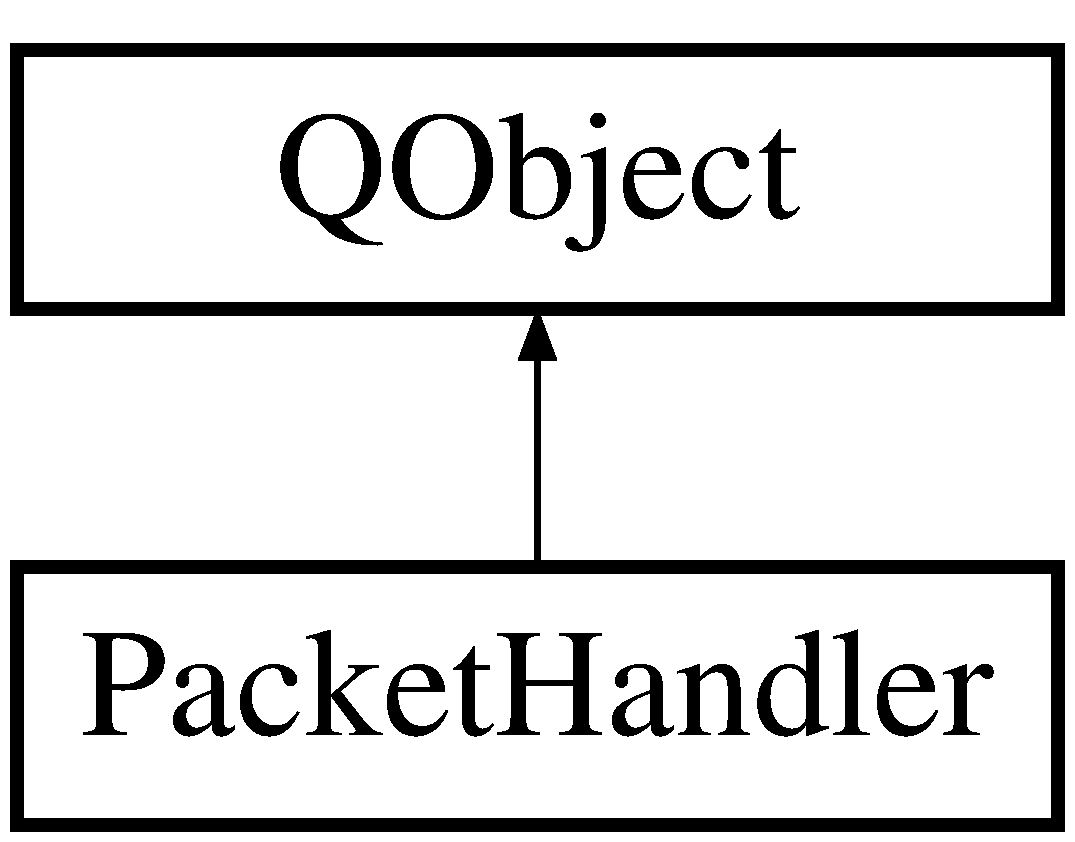
\includegraphics[height=2.000000cm]{class_packet_handler}
\end{center}
\end{figure}
\subsection*{Signale}
\begin{DoxyCompactItemize}
\item 
void \hyperlink{class_packet_handler_a7434b94845f0389703fa4d85e8487372}{read\+Field} (Q\+Byte\+Array p\+\_\+field)
\begin{DoxyCompactList}\small\item\em Signal das emittiert wird, wenn das Spielfeldsynchronisations-\/\+Paket verarbeitet wird. \end{DoxyCompactList}\item 
void \hyperlink{class_packet_handler_a766789a5ff926bee167e308b620f8807}{read\+Scores} (Q\+Byte\+Array p\+\_\+scores)
\begin{DoxyCompactList}\small\item\em Signal das emittiert wird, wenn das Punktestandsynchronisations-\/\+Paket verarbeitet wird. \end{DoxyCompactList}\item 
void \hyperlink{class_packet_handler_a8cb91da2e7e174f5b781d5338a54427e}{read\+Click} (Q\+Tcp\+Socket $\ast$p\+\_\+socket, Q\+Byte\+Array p\+\_\+cards)
\begin{DoxyCompactList}\small\item\em Signal das emittiert wird, wenn ein Klick-\/\+Paket verarbeitet wird. \end{DoxyCompactList}\item 
void \hyperlink{class_packet_handler_a84c59146583fc6ee254940cce4377b54}{read\+Game\+Started\+Packet} ()
\begin{DoxyCompactList}\small\item\em Signal das emittiert wird, wenn das Spielstarten-\/\+Paket verarbeitet wird. \end{DoxyCompactList}\item 
void \hyperlink{class_packet_handler_aa47688eb98584d262f5ba2f98f019105}{read\+Game\+Finished\+Packet} ()
\begin{DoxyCompactList}\small\item\em Signal das emittiert wird, wenn das Spielbeenden-\/\+Paket verarbeitet wird. \end{DoxyCompactList}\item 
void \hyperlink{class_packet_handler_abc467ba059a00877d8fae31672395ac4}{read\+Deck\+Length} (short p\+\_\+deck\+Length)
\begin{DoxyCompactList}\small\item\em Signal das emittiert wird, wenn das Deckgrößen-\/\+Paket verarbeitet wird. \end{DoxyCompactList}\item 
void \hyperlink{class_packet_handler_acba72c3a586146653ad0b6c0851dbc0c}{read\+Locked\+Packet} ()
\begin{DoxyCompactList}\small\item\em Signal das emittiert wird, wenn das Eingabensperr-\/\+Paket verarbeitet wird. \end{DoxyCompactList}\item 
void \hyperlink{class_packet_handler_a309f2c1cd016039c1fe8b38d75b3ef7c}{read\+Unlocked\+Packet} ()
\begin{DoxyCompactList}\small\item\em Signal das emittiert wird, wenn das Eingabenentsperr-\/\+Paket verarbeitet wird. \end{DoxyCompactList}\item 
void \hyperlink{class_packet_handler_aceaa87f977376e769e840db3e0756bfe}{read\+Turn\+Packet} (Q\+Tcp\+Socket $\ast$p\+\_\+socket)
\begin{DoxyCompactList}\small\item\em Signal das emittiert wird, wenn das Spieler-\/\+Am-\/\+Zug-\/\+Paket verarbeitet wird. \end{DoxyCompactList}\end{DoxyCompactItemize}
\subsection*{Öffentliche Methoden}
\begin{DoxyCompactItemize}
\item 
\hyperlink{class_packet_handler_a4728b3f54723e7f05e947eb56433d4b5}{Packet\+Handler} (Q\+Object $\ast$parent=0)
\begin{DoxyCompactList}\small\item\em Konstruktor zum Erzeugen einer Packet\+Handler-\/\+Instanz. \end{DoxyCompactList}\item 
void \hyperlink{class_packet_handler_a4d948da50131eeef0d977e0693ff9741}{process\+Packets} (Q\+Byte\+Array p\+\_\+packets, Q\+Tcp\+Socket $\ast$p\+\_\+socket=nullptr)
\begin{DoxyCompactList}\small\item\em Teilt den Datenstrom in die einzelnen Pakete auf und verarbeitet diese dann. \end{DoxyCompactList}\item 
Q\+Byte\+Array \hyperlink{class_packet_handler_a9e2e51aa1b548ec1b209ee682bdd4c54}{make\+F\+S\+Packet} (std\+::list$<$ \hyperlink{class_card}{Card} $\ast$ $>$ \&p\+\_\+field)
\begin{DoxyCompactList}\small\item\em Erzeugt ein Paket für die Spielfeldsynchronisation, anhand einer Liste aus Karte. \end{DoxyCompactList}\item 
Q\+Byte\+Array \hyperlink{class_packet_handler_abd77784148000bbe33af457c09a05022}{make\+Click\+Packet} (Q\+Byte\+Array p\+\_\+cards)
\begin{DoxyCompactList}\small\item\em Erzeugt ein Paket das eine Set-\/\+Auswahl darstellt. \end{DoxyCompactList}\item 
Q\+Byte\+Array \hyperlink{class_packet_handler_a256842b9c4243360441366ae04838b0d}{make\+Scores\+Packet} (Q\+Byte\+Array p\+\_\+scores)
\begin{DoxyCompactList}\small\item\em Erzeugt ein Paket, für die Punkte-\/\+Synchronisation. \end{DoxyCompactList}\item 
Q\+Byte\+Array \hyperlink{class_packet_handler_aef3b383774fb1894dcd99dd40b3f735a}{make\+Game\+Started\+Packet} ()
\begin{DoxyCompactList}\small\item\em Erzeugt eine Paket das den Start des Spiels darstellt. \end{DoxyCompactList}\item 
Q\+Byte\+Array \hyperlink{class_packet_handler_ad8cdb7008eb99e5dfc5383746d18b4f3}{make\+Game\+Finished\+Packet} ()
\begin{DoxyCompactList}\small\item\em Erzeugt ein Paket, um das Spielende anzusagen. \end{DoxyCompactList}\item 
Q\+Byte\+Array \hyperlink{class_packet_handler_a3de99e5e6f714e26f558c99bfdfc6968}{make\+Deck\+Length\+Packet} (short p\+\_\+deck\+Length)
\begin{DoxyCompactList}\small\item\em Erzeugt ein Paket das die Anzahl der im Deck beinhalteten Karten darstellt. \end{DoxyCompactList}\item 
Q\+Byte\+Array \hyperlink{class_packet_handler_ad64f92836fdc7415ce7b012065bd985b}{make\+Input\+Locked\+Packet} ()
\begin{DoxyCompactList}\small\item\em Erzeugt ein Paket das die Sperrung der Eingaben bewirkt. \end{DoxyCompactList}\item 
Q\+Byte\+Array \hyperlink{class_packet_handler_a49c990160b529af585b201b8690058ef}{make\+Input\+Unlocked\+Packet} ()
\begin{DoxyCompactList}\small\item\em Erzeugt ein Paket das die Entsperrung der Eingaben bewirkt. \end{DoxyCompactList}\item 
Q\+Byte\+Array \hyperlink{class_packet_handler_a76a8c456652beb81888ddb02718db34c}{make\+Turn\+Packet} ()
\begin{DoxyCompactList}\small\item\em Erzeugt ein Paket das angibt, dass ein Spieler ein Set auswählen möchte. \end{DoxyCompactList}\end{DoxyCompactItemize}


\subsection{Ausführliche Beschreibung}
Die Packet\+Handler-\/\+Klasse dient zur Verwaltung von ein-\/ bzw. ausgehenden Paketen.~\newline
 Werden bestimmte Pakettypen erkannt, so werden die entsprechenden Signale emittiert,~\newline
 und dadurch die Slots in den externen Klassen aufgerufen. 

\subsection{Beschreibung der Konstruktoren und Destruktoren}
\hypertarget{class_packet_handler_a4728b3f54723e7f05e947eb56433d4b5}{}\index{Packet\+Handler@{Packet\+Handler}!Packet\+Handler@{Packet\+Handler}}
\index{Packet\+Handler@{Packet\+Handler}!Packet\+Handler@{Packet\+Handler}}
\subsubsection[{Packet\+Handler}]{\setlength{\rightskip}{0pt plus 5cm}Packet\+Handler\+::\+Packet\+Handler (
\begin{DoxyParamCaption}
\item[{Q\+Object $\ast$}]{parent = {\ttfamily 0}}
\end{DoxyParamCaption}
)\hspace{0.3cm}{\ttfamily [explicit]}}\label{class_packet_handler_a4728b3f54723e7f05e947eb56433d4b5}


Konstruktor zum Erzeugen einer Packet\+Handler-\/\+Instanz. 


\begin{DoxyParams}{Parameter}
{\em parent} & Elternteil des Packet\+Handlers \\
\hline
\end{DoxyParams}


\subsection{Dokumentation der Elementfunktionen}
\hypertarget{class_packet_handler_abd77784148000bbe33af457c09a05022}{}\index{Packet\+Handler@{Packet\+Handler}!make\+Click\+Packet@{make\+Click\+Packet}}
\index{make\+Click\+Packet@{make\+Click\+Packet}!Packet\+Handler@{Packet\+Handler}}
\subsubsection[{make\+Click\+Packet}]{\setlength{\rightskip}{0pt plus 5cm}Q\+Byte\+Array Packet\+Handler\+::make\+Click\+Packet (
\begin{DoxyParamCaption}
\item[{Q\+Byte\+Array}]{p\+\_\+cards}
\end{DoxyParamCaption}
)}\label{class_packet_handler_abd77784148000bbe33af457c09a05022}


Erzeugt ein Paket das eine Set-\/\+Auswahl darstellt. 


\begin{DoxyParams}{Parameter}
{\em p\+\_\+cards} & Ausgewählte Karten \\
\hline
\end{DoxyParams}
\begin{DoxyReturn}{Rückgabe}
Paket 
\end{DoxyReturn}
\hypertarget{class_packet_handler_a3de99e5e6f714e26f558c99bfdfc6968}{}\index{Packet\+Handler@{Packet\+Handler}!make\+Deck\+Length\+Packet@{make\+Deck\+Length\+Packet}}
\index{make\+Deck\+Length\+Packet@{make\+Deck\+Length\+Packet}!Packet\+Handler@{Packet\+Handler}}
\subsubsection[{make\+Deck\+Length\+Packet}]{\setlength{\rightskip}{0pt plus 5cm}Q\+Byte\+Array Packet\+Handler\+::make\+Deck\+Length\+Packet (
\begin{DoxyParamCaption}
\item[{short}]{p\+\_\+deck\+Length}
\end{DoxyParamCaption}
)}\label{class_packet_handler_a3de99e5e6f714e26f558c99bfdfc6968}


Erzeugt ein Paket das die Anzahl der im Deck beinhalteten Karten darstellt. 


\begin{DoxyParams}{Parameter}
{\em p\+\_\+deck\+Length} & Deckgröße \\
\hline
\end{DoxyParams}
\begin{DoxyReturn}{Rückgabe}
Paket 
\end{DoxyReturn}
\hypertarget{class_packet_handler_a9e2e51aa1b548ec1b209ee682bdd4c54}{}\index{Packet\+Handler@{Packet\+Handler}!make\+F\+S\+Packet@{make\+F\+S\+Packet}}
\index{make\+F\+S\+Packet@{make\+F\+S\+Packet}!Packet\+Handler@{Packet\+Handler}}
\subsubsection[{make\+F\+S\+Packet}]{\setlength{\rightskip}{0pt plus 5cm}Q\+Byte\+Array Packet\+Handler\+::make\+F\+S\+Packet (
\begin{DoxyParamCaption}
\item[{std\+::list$<$ {\bf Card} $\ast$ $>$ \&}]{p\+\_\+field}
\end{DoxyParamCaption}
)}\label{class_packet_handler_a9e2e51aa1b548ec1b209ee682bdd4c54}


Erzeugt ein Paket für die Spielfeldsynchronisation, anhand einer Liste aus Karte. 


\begin{DoxyParams}{Parameter}
{\em p\+\_\+field} & Liste aus Karten -\/ Spielfeld \\
\hline
\end{DoxyParams}
\begin{DoxyReturn}{Rückgabe}
Paket 
\end{DoxyReturn}
\hypertarget{class_packet_handler_ad8cdb7008eb99e5dfc5383746d18b4f3}{}\index{Packet\+Handler@{Packet\+Handler}!make\+Game\+Finished\+Packet@{make\+Game\+Finished\+Packet}}
\index{make\+Game\+Finished\+Packet@{make\+Game\+Finished\+Packet}!Packet\+Handler@{Packet\+Handler}}
\subsubsection[{make\+Game\+Finished\+Packet}]{\setlength{\rightskip}{0pt plus 5cm}Q\+Byte\+Array Packet\+Handler\+::make\+Game\+Finished\+Packet (
\begin{DoxyParamCaption}
{}
\end{DoxyParamCaption}
)}\label{class_packet_handler_ad8cdb7008eb99e5dfc5383746d18b4f3}


Erzeugt ein Paket, um das Spielende anzusagen. 

\begin{DoxyReturn}{Rückgabe}
Paket 
\end{DoxyReturn}
\hypertarget{class_packet_handler_aef3b383774fb1894dcd99dd40b3f735a}{}\index{Packet\+Handler@{Packet\+Handler}!make\+Game\+Started\+Packet@{make\+Game\+Started\+Packet}}
\index{make\+Game\+Started\+Packet@{make\+Game\+Started\+Packet}!Packet\+Handler@{Packet\+Handler}}
\subsubsection[{make\+Game\+Started\+Packet}]{\setlength{\rightskip}{0pt plus 5cm}Q\+Byte\+Array Packet\+Handler\+::make\+Game\+Started\+Packet (
\begin{DoxyParamCaption}
{}
\end{DoxyParamCaption}
)}\label{class_packet_handler_aef3b383774fb1894dcd99dd40b3f735a}


Erzeugt eine Paket das den Start des Spiels darstellt. 

\begin{DoxyReturn}{Rückgabe}
Paket 
\end{DoxyReturn}
\hypertarget{class_packet_handler_ad64f92836fdc7415ce7b012065bd985b}{}\index{Packet\+Handler@{Packet\+Handler}!make\+Input\+Locked\+Packet@{make\+Input\+Locked\+Packet}}
\index{make\+Input\+Locked\+Packet@{make\+Input\+Locked\+Packet}!Packet\+Handler@{Packet\+Handler}}
\subsubsection[{make\+Input\+Locked\+Packet}]{\setlength{\rightskip}{0pt plus 5cm}Q\+Byte\+Array Packet\+Handler\+::make\+Input\+Locked\+Packet (
\begin{DoxyParamCaption}
{}
\end{DoxyParamCaption}
)}\label{class_packet_handler_ad64f92836fdc7415ce7b012065bd985b}


Erzeugt ein Paket das die Sperrung der Eingaben bewirkt. 

\begin{DoxyReturn}{Rückgabe}
Paket 
\end{DoxyReturn}
\hypertarget{class_packet_handler_a49c990160b529af585b201b8690058ef}{}\index{Packet\+Handler@{Packet\+Handler}!make\+Input\+Unlocked\+Packet@{make\+Input\+Unlocked\+Packet}}
\index{make\+Input\+Unlocked\+Packet@{make\+Input\+Unlocked\+Packet}!Packet\+Handler@{Packet\+Handler}}
\subsubsection[{make\+Input\+Unlocked\+Packet}]{\setlength{\rightskip}{0pt plus 5cm}Q\+Byte\+Array Packet\+Handler\+::make\+Input\+Unlocked\+Packet (
\begin{DoxyParamCaption}
{}
\end{DoxyParamCaption}
)}\label{class_packet_handler_a49c990160b529af585b201b8690058ef}


Erzeugt ein Paket das die Entsperrung der Eingaben bewirkt. 

\begin{DoxyReturn}{Rückgabe}
Paket 
\end{DoxyReturn}
\hypertarget{class_packet_handler_a256842b9c4243360441366ae04838b0d}{}\index{Packet\+Handler@{Packet\+Handler}!make\+Scores\+Packet@{make\+Scores\+Packet}}
\index{make\+Scores\+Packet@{make\+Scores\+Packet}!Packet\+Handler@{Packet\+Handler}}
\subsubsection[{make\+Scores\+Packet}]{\setlength{\rightskip}{0pt plus 5cm}Q\+Byte\+Array Packet\+Handler\+::make\+Scores\+Packet (
\begin{DoxyParamCaption}
\item[{Q\+Byte\+Array}]{p\+\_\+scores}
\end{DoxyParamCaption}
)}\label{class_packet_handler_a256842b9c4243360441366ae04838b0d}


Erzeugt ein Paket, für die Punkte-\/\+Synchronisation. 


\begin{DoxyParams}{Parameter}
{\em p\+\_\+scores} & Die Punkte aller Spieler \\
\hline
\end{DoxyParams}
\begin{DoxyReturn}{Rückgabe}
Paket 
\end{DoxyReturn}
\hypertarget{class_packet_handler_a76a8c456652beb81888ddb02718db34c}{}\index{Packet\+Handler@{Packet\+Handler}!make\+Turn\+Packet@{make\+Turn\+Packet}}
\index{make\+Turn\+Packet@{make\+Turn\+Packet}!Packet\+Handler@{Packet\+Handler}}
\subsubsection[{make\+Turn\+Packet}]{\setlength{\rightskip}{0pt plus 5cm}Q\+Byte\+Array Packet\+Handler\+::make\+Turn\+Packet (
\begin{DoxyParamCaption}
{}
\end{DoxyParamCaption}
)}\label{class_packet_handler_a76a8c456652beb81888ddb02718db34c}


Erzeugt ein Paket das angibt, dass ein Spieler ein Set auswählen möchte. 

\begin{DoxyReturn}{Rückgabe}
Paket 
\end{DoxyReturn}
\hypertarget{class_packet_handler_a4d948da50131eeef0d977e0693ff9741}{}\index{Packet\+Handler@{Packet\+Handler}!process\+Packets@{process\+Packets}}
\index{process\+Packets@{process\+Packets}!Packet\+Handler@{Packet\+Handler}}
\subsubsection[{process\+Packets}]{\setlength{\rightskip}{0pt plus 5cm}void Packet\+Handler\+::process\+Packets (
\begin{DoxyParamCaption}
\item[{Q\+Byte\+Array}]{p\+\_\+packets, }
\item[{Q\+Tcp\+Socket $\ast$}]{p\+\_\+socket = {\ttfamily nullptr}}
\end{DoxyParamCaption}
)}\label{class_packet_handler_a4d948da50131eeef0d977e0693ff9741}


Teilt den Datenstrom in die einzelnen Pakete auf und verarbeitet diese dann. 


\begin{DoxyParams}{Parameter}
{\em p\+\_\+packets} & Datenstrom \\
\hline
{\em p\+\_\+socket} & Absender \\
\hline
\end{DoxyParams}
\begin{DoxySeeAlso}{Siehe auch}
process\+Packet 
\end{DoxySeeAlso}
\hypertarget{class_packet_handler_a8cb91da2e7e174f5b781d5338a54427e}{}\index{Packet\+Handler@{Packet\+Handler}!read\+Click@{read\+Click}}
\index{read\+Click@{read\+Click}!Packet\+Handler@{Packet\+Handler}}
\subsubsection[{read\+Click}]{\setlength{\rightskip}{0pt plus 5cm}void Packet\+Handler\+::read\+Click (
\begin{DoxyParamCaption}
\item[{Q\+Tcp\+Socket $\ast$}]{p\+\_\+socket, }
\item[{Q\+Byte\+Array}]{p\+\_\+cards}
\end{DoxyParamCaption}
)\hspace{0.3cm}{\ttfamily [signal]}}\label{class_packet_handler_a8cb91da2e7e174f5b781d5338a54427e}


Signal das emittiert wird, wenn ein Klick-\/\+Paket verarbeitet wird. 


\begin{DoxyParams}{Parameter}
{\em p\+\_\+socket} & Absender \\
\hline
{\em p\+\_\+cards} & Ausgewählte Karten \\
\hline
\end{DoxyParams}
\hypertarget{class_packet_handler_abc467ba059a00877d8fae31672395ac4}{}\index{Packet\+Handler@{Packet\+Handler}!read\+Deck\+Length@{read\+Deck\+Length}}
\index{read\+Deck\+Length@{read\+Deck\+Length}!Packet\+Handler@{Packet\+Handler}}
\subsubsection[{read\+Deck\+Length}]{\setlength{\rightskip}{0pt plus 5cm}void Packet\+Handler\+::read\+Deck\+Length (
\begin{DoxyParamCaption}
\item[{short}]{p\+\_\+deck\+Length}
\end{DoxyParamCaption}
)\hspace{0.3cm}{\ttfamily [signal]}}\label{class_packet_handler_abc467ba059a00877d8fae31672395ac4}


Signal das emittiert wird, wenn das Deckgrößen-\/\+Paket verarbeitet wird. 


\begin{DoxyParams}{Parameter}
{\em p\+\_\+deck\+Length} & Deckgröße \\
\hline
\end{DoxyParams}
\hypertarget{class_packet_handler_a7434b94845f0389703fa4d85e8487372}{}\index{Packet\+Handler@{Packet\+Handler}!read\+Field@{read\+Field}}
\index{read\+Field@{read\+Field}!Packet\+Handler@{Packet\+Handler}}
\subsubsection[{read\+Field}]{\setlength{\rightskip}{0pt plus 5cm}void Packet\+Handler\+::read\+Field (
\begin{DoxyParamCaption}
\item[{Q\+Byte\+Array}]{p\+\_\+field}
\end{DoxyParamCaption}
)\hspace{0.3cm}{\ttfamily [signal]}}\label{class_packet_handler_a7434b94845f0389703fa4d85e8487372}


Signal das emittiert wird, wenn das Spielfeldsynchronisations-\/\+Paket verarbeitet wird. 


\begin{DoxyParams}{Parameter}
{\em p\+\_\+field} & Spielfeld \\
\hline
\end{DoxyParams}
\hypertarget{class_packet_handler_aa47688eb98584d262f5ba2f98f019105}{}\index{Packet\+Handler@{Packet\+Handler}!read\+Game\+Finished\+Packet@{read\+Game\+Finished\+Packet}}
\index{read\+Game\+Finished\+Packet@{read\+Game\+Finished\+Packet}!Packet\+Handler@{Packet\+Handler}}
\subsubsection[{read\+Game\+Finished\+Packet}]{\setlength{\rightskip}{0pt plus 5cm}void Packet\+Handler\+::read\+Game\+Finished\+Packet (
\begin{DoxyParamCaption}
{}
\end{DoxyParamCaption}
)\hspace{0.3cm}{\ttfamily [signal]}}\label{class_packet_handler_aa47688eb98584d262f5ba2f98f019105}


Signal das emittiert wird, wenn das Spielbeenden-\/\+Paket verarbeitet wird. 

\hypertarget{class_packet_handler_a84c59146583fc6ee254940cce4377b54}{}\index{Packet\+Handler@{Packet\+Handler}!read\+Game\+Started\+Packet@{read\+Game\+Started\+Packet}}
\index{read\+Game\+Started\+Packet@{read\+Game\+Started\+Packet}!Packet\+Handler@{Packet\+Handler}}
\subsubsection[{read\+Game\+Started\+Packet}]{\setlength{\rightskip}{0pt plus 5cm}void Packet\+Handler\+::read\+Game\+Started\+Packet (
\begin{DoxyParamCaption}
{}
\end{DoxyParamCaption}
)\hspace{0.3cm}{\ttfamily [signal]}}\label{class_packet_handler_a84c59146583fc6ee254940cce4377b54}


Signal das emittiert wird, wenn das Spielstarten-\/\+Paket verarbeitet wird. 

\hypertarget{class_packet_handler_acba72c3a586146653ad0b6c0851dbc0c}{}\index{Packet\+Handler@{Packet\+Handler}!read\+Locked\+Packet@{read\+Locked\+Packet}}
\index{read\+Locked\+Packet@{read\+Locked\+Packet}!Packet\+Handler@{Packet\+Handler}}
\subsubsection[{read\+Locked\+Packet}]{\setlength{\rightskip}{0pt plus 5cm}void Packet\+Handler\+::read\+Locked\+Packet (
\begin{DoxyParamCaption}
{}
\end{DoxyParamCaption}
)\hspace{0.3cm}{\ttfamily [signal]}}\label{class_packet_handler_acba72c3a586146653ad0b6c0851dbc0c}


Signal das emittiert wird, wenn das Eingabensperr-\/\+Paket verarbeitet wird. 

\hypertarget{class_packet_handler_a766789a5ff926bee167e308b620f8807}{}\index{Packet\+Handler@{Packet\+Handler}!read\+Scores@{read\+Scores}}
\index{read\+Scores@{read\+Scores}!Packet\+Handler@{Packet\+Handler}}
\subsubsection[{read\+Scores}]{\setlength{\rightskip}{0pt plus 5cm}void Packet\+Handler\+::read\+Scores (
\begin{DoxyParamCaption}
\item[{Q\+Byte\+Array}]{p\+\_\+scores}
\end{DoxyParamCaption}
)\hspace{0.3cm}{\ttfamily [signal]}}\label{class_packet_handler_a766789a5ff926bee167e308b620f8807}


Signal das emittiert wird, wenn das Punktestandsynchronisations-\/\+Paket verarbeitet wird. 


\begin{DoxyParams}{Parameter}
{\em p\+\_\+scores} & Punktestand \\
\hline
\end{DoxyParams}
\hypertarget{class_packet_handler_aceaa87f977376e769e840db3e0756bfe}{}\index{Packet\+Handler@{Packet\+Handler}!read\+Turn\+Packet@{read\+Turn\+Packet}}
\index{read\+Turn\+Packet@{read\+Turn\+Packet}!Packet\+Handler@{Packet\+Handler}}
\subsubsection[{read\+Turn\+Packet}]{\setlength{\rightskip}{0pt plus 5cm}void Packet\+Handler\+::read\+Turn\+Packet (
\begin{DoxyParamCaption}
\item[{Q\+Tcp\+Socket $\ast$}]{p\+\_\+socket}
\end{DoxyParamCaption}
)\hspace{0.3cm}{\ttfamily [signal]}}\label{class_packet_handler_aceaa87f977376e769e840db3e0756bfe}


Signal das emittiert wird, wenn das Spieler-\/\+Am-\/\+Zug-\/\+Paket verarbeitet wird. 


\begin{DoxyParams}{Parameter}
{\em p\+\_\+socket} & Spieler, der am Zug ist \\
\hline
\end{DoxyParams}
\hypertarget{class_packet_handler_a309f2c1cd016039c1fe8b38d75b3ef7c}{}\index{Packet\+Handler@{Packet\+Handler}!read\+Unlocked\+Packet@{read\+Unlocked\+Packet}}
\index{read\+Unlocked\+Packet@{read\+Unlocked\+Packet}!Packet\+Handler@{Packet\+Handler}}
\subsubsection[{read\+Unlocked\+Packet}]{\setlength{\rightskip}{0pt plus 5cm}void Packet\+Handler\+::read\+Unlocked\+Packet (
\begin{DoxyParamCaption}
{}
\end{DoxyParamCaption}
)\hspace{0.3cm}{\ttfamily [signal]}}\label{class_packet_handler_a309f2c1cd016039c1fe8b38d75b3ef7c}


Signal das emittiert wird, wenn das Eingabenentsperr-\/\+Paket verarbeitet wird. 



Die Dokumentation für diese Klasse wurde erzeugt aufgrund der Dateien\+:\begin{DoxyCompactItemize}
\item 
src/\hyperlink{packethandler_8hpp}{packethandler.\+hpp}\item 
src/\hyperlink{packethandler_8cpp}{packethandler.\+cpp}\end{DoxyCompactItemize}

\hypertarget{class_player}{}\section{Player Klassenreferenz}
\label{class_player}\index{Player@{Player}}


Spieler-\/\+Klasse.  




{\ttfamily \#include $<$player.\+hpp$>$}

Klassendiagramm für Player\+:\begin{figure}[H]
\begin{center}
\leavevmode
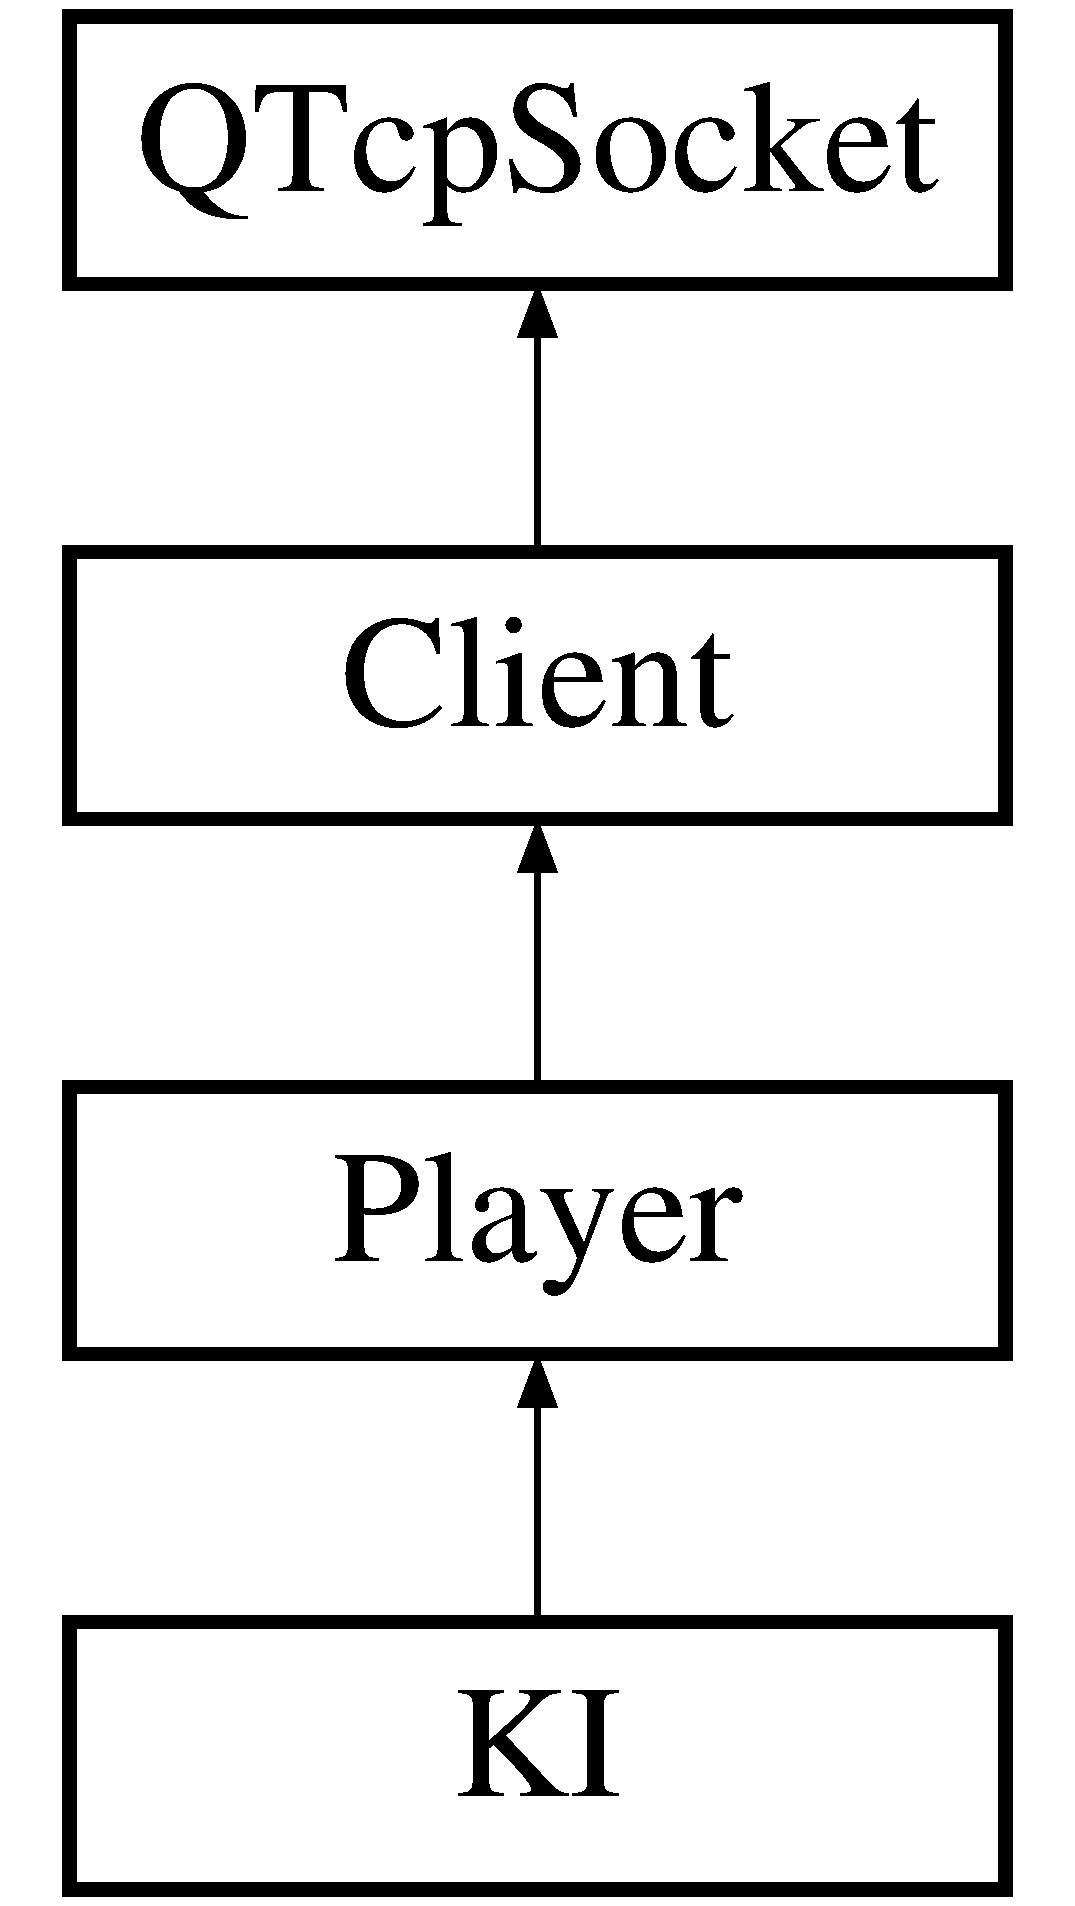
\includegraphics[height=4.000000cm]{class_player}
\end{center}
\end{figure}
\subsection*{Öffentliche Methoden}
\begin{DoxyCompactItemize}
\item 
void \hyperlink{class_player_ae688e0cb60be7901e195d7881b4d39ce}{send\+Click\+Packet} (Q\+Byte\+Array p\+\_\+cards)
\begin{DoxyCompactList}\small\item\em Sendet ein Paket an den \hyperlink{class_server}{Server}, in dem die ausgewählten Karten drinnenstehen.~\newline
 Der \hyperlink{class_server}{Server} überprüft diese auf ein Set und erhöht und senkt dementsprechend die Punktzahl des Spielers. \end{DoxyCompactList}\item 
void \hyperlink{class_player_a08220f4cd6aa057071371a7c815a63dd}{send\+Turn\+Packet} ()
\begin{DoxyCompactList}\small\item\em Sendet ein Paket an den \hyperlink{class_server}{Server}, dass dafür steht, dass dieser Spieler eine Set-\/\+Auswahl trifft. \end{DoxyCompactList}\item 
\hyperlink{class_player_af07248b94d3f4ad62841d6dae90f5def}{Player} (Q\+Object $\ast$p\+\_\+parent=0, Q\+Host\+Address p\+\_\+ip=Q\+Host\+Address\+::\+Local\+Host, int p\+\_\+port=1337)
\begin{DoxyCompactList}\small\item\em Konstruktor zum Erzeugen einer Player-\/\+Klasse. \end{DoxyCompactList}\end{DoxyCompactItemize}
\subsection*{Weitere Geerbte Elemente}


\subsection{Ausführliche Beschreibung}
Spieler-\/\+Klasse. 

\subsection{Beschreibung der Konstruktoren und Destruktoren}
\hypertarget{class_player_af07248b94d3f4ad62841d6dae90f5def}{}\index{Player@{Player}!Player@{Player}}
\index{Player@{Player}!Player@{Player}}
\subsubsection[{Player}]{\setlength{\rightskip}{0pt plus 5cm}Player\+::\+Player (
\begin{DoxyParamCaption}
\item[{Q\+Object $\ast$}]{p\+\_\+parent = {\ttfamily 0}, }
\item[{Q\+Host\+Address}]{p\+\_\+ip = {\ttfamily QHostAddress\+:\+:LocalHost}, }
\item[{int}]{p\+\_\+port = {\ttfamily 1337}}
\end{DoxyParamCaption}
)}\label{class_player_af07248b94d3f4ad62841d6dae90f5def}


Konstruktor zum Erzeugen einer Player-\/\+Klasse. 


\begin{DoxyParams}{Parameter}
{\em p\+\_\+parent} & Elternteil des Players \\
\hline
{\em p\+\_\+ip} & I\+P-\/\+Adresse des Servers \\
\hline
{\em p\+\_\+port} & Port über den die Verbindung läuft \\
\hline
\end{DoxyParams}


\subsection{Dokumentation der Elementfunktionen}
\hypertarget{class_player_ae688e0cb60be7901e195d7881b4d39ce}{}\index{Player@{Player}!send\+Click\+Packet@{send\+Click\+Packet}}
\index{send\+Click\+Packet@{send\+Click\+Packet}!Player@{Player}}
\subsubsection[{send\+Click\+Packet}]{\setlength{\rightskip}{0pt plus 5cm}void Player\+::send\+Click\+Packet (
\begin{DoxyParamCaption}
\item[{Q\+Byte\+Array}]{p\+\_\+cards}
\end{DoxyParamCaption}
)\hspace{0.3cm}{\ttfamily [virtual]}}\label{class_player_ae688e0cb60be7901e195d7881b4d39ce}


Sendet ein Paket an den \hyperlink{class_server}{Server}, in dem die ausgewählten Karten drinnenstehen.~\newline
 Der \hyperlink{class_server}{Server} überprüft diese auf ein Set und erhöht und senkt dementsprechend die Punktzahl des Spielers. 


\begin{DoxyParams}{Parameter}
{\em p\+\_\+cards} & Angeklickte Karten \\
\hline
\end{DoxyParams}
\begin{DoxySeeAlso}{Siehe auch}
\hyperlink{class_packet_handler_abd77784148000bbe33af457c09a05022}{Packet\+Handler\+::make\+Click\+Packet} 
\end{DoxySeeAlso}


Implementiert \hyperlink{class_client_ac3b60506d2f900a3490a05425f392914}{Client}.

\hypertarget{class_player_a08220f4cd6aa057071371a7c815a63dd}{}\index{Player@{Player}!send\+Turn\+Packet@{send\+Turn\+Packet}}
\index{send\+Turn\+Packet@{send\+Turn\+Packet}!Player@{Player}}
\subsubsection[{send\+Turn\+Packet}]{\setlength{\rightskip}{0pt plus 5cm}void Player\+::send\+Turn\+Packet (
\begin{DoxyParamCaption}
{}
\end{DoxyParamCaption}
)\hspace{0.3cm}{\ttfamily [virtual]}}\label{class_player_a08220f4cd6aa057071371a7c815a63dd}


Sendet ein Paket an den \hyperlink{class_server}{Server}, dass dafür steht, dass dieser Spieler eine Set-\/\+Auswahl trifft. 



Implementiert \hyperlink{class_client_a62fc6262c8e9f0e9a0b2811a9c6fa8b0}{Client}.



Die Dokumentation für diese Klasse wurde erzeugt aufgrund der Dateien\+:\begin{DoxyCompactItemize}
\item 
src/\hyperlink{player_8hpp}{player.\+hpp}\item 
src/\hyperlink{player_8cpp}{player.\+cpp}\end{DoxyCompactItemize}

\hypertarget{class_server}{}\section{Server Klassenreferenz}
\label{class_server}\index{Server@{Server}}


Die abstrakte Klasse \hyperlink{class_server}{Server}, steht für den \hyperlink{class_server}{Server} des Spiels.  




{\ttfamily \#include $<$server.\+hpp$>$}

Klassendiagramm für Server\+:\begin{figure}[H]
\begin{center}
\leavevmode
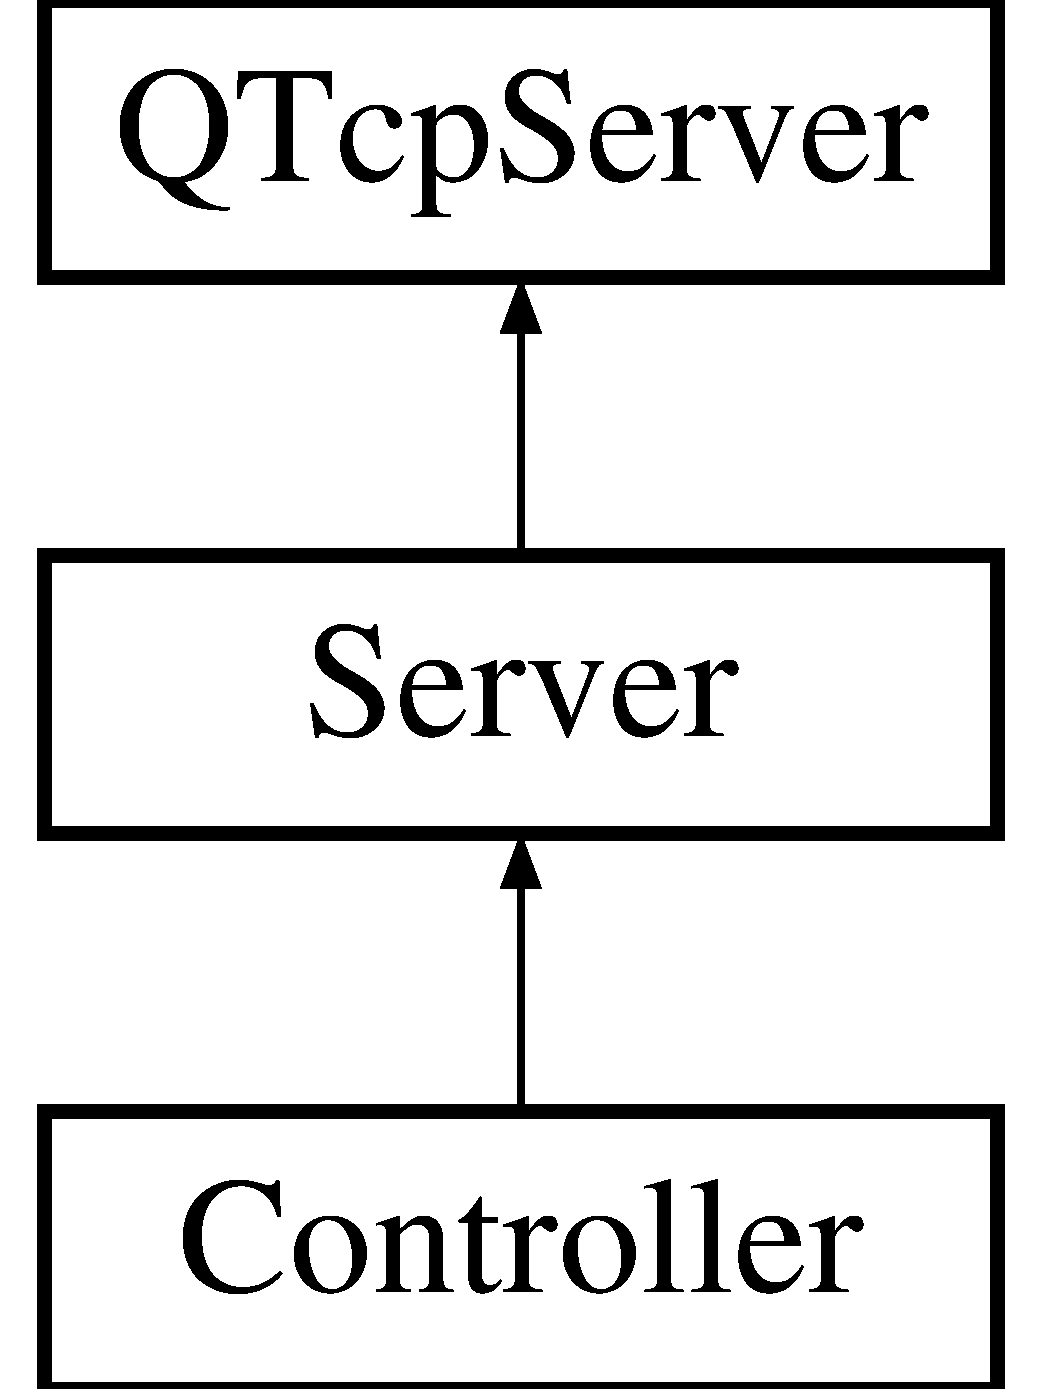
\includegraphics[height=3.000000cm]{class_server}
\end{center}
\end{figure}
\subsection*{Öffentliche Slots}
\begin{DoxyCompactItemize}
\item 
void \hyperlink{class_server_a278a1ed6357a7d773c1d9d452f7d8cf1}{new\+Con} ()
\begin{DoxyCompactList}\small\item\em Wird aufgerufen, wenn eine neue Verbindung zur Verfügung steht. \end{DoxyCompactList}\item 
void \hyperlink{class_server_ac67d866fb14c4644acd1098bacfadeee}{on\+Ready\+Read} ()
\begin{DoxyCompactList}\small\item\em Wird aufgerufen, sobald der Buffer mit den eingehenden Paketen lesebereit ist. \end{DoxyCompactList}\item 
virtual void \hyperlink{class_server_aabd6ee61f3530f06cf7664a283f40f33}{retrieve\+Click} (Q\+Tcp\+Socket $\ast$p\+\_\+client, Q\+Byte\+Array p\+\_\+cards)=0
\begin{DoxyCompactList}\small\item\em Wird aufgerufen, wenn ein Set ausgewählt wurde.~\newline
 Das Set wird überprüft und dementsprechend Punkte gutgeschrieben oder abgezogen. \end{DoxyCompactList}\item 
virtual void \hyperlink{class_server_a5455bcd1eeb8acbf5d3b6d91420b44d4}{retrieve\+Player\+Turn} (Q\+Tcp\+Socket $\ast$p\+\_\+socket)=0
\begin{DoxyCompactList}\small\item\em Wird aufgerufen, sobald ein Spieler ein Set auswählen möchte. \end{DoxyCompactList}\end{DoxyCompactItemize}
\subsection*{Öffentliche Methoden}
\begin{DoxyCompactItemize}
\item 
virtual void \hyperlink{class_server_a1be346a3252468e445f8f809d1c912e7}{send\+Game\+Started\+Packet} ()=0
\begin{DoxyCompactList}\small\item\em Sendet das Paket, um das Spiel zu starten. \end{DoxyCompactList}\item 
\hyperlink{class_server_a9fc4c94bf5687657b7d1eea35334ed44}{Server} (Q\+Object $\ast$parent=0, int p\+\_\+port=1337)
\begin{DoxyCompactList}\small\item\em Konstruktor zum Erzeugen einer Server-\/\+Instanz. \end{DoxyCompactList}\end{DoxyCompactItemize}
\subsection*{Geschützte Typen}
\begin{DoxyCompactItemize}
\item 
typedef std\+::list$<$ \hyperlink{class_card}{Card} $\ast$ $>$ \hyperlink{class_server_a2b2ff2c4678bdca3599c3feb5efdaff7}{Cards}
\begin{DoxyCompactList}\small\item\em Typdefinition Cards. \end{DoxyCompactList}\item 
typedef std\+::tuple$<$ Q\+Tcp\+Socket $\ast$, short, \hyperlink{class_server_a2b2ff2c4678bdca3599c3feb5efdaff7}{Cards} $>$ \hyperlink{class_server_a31786b51863a753101d409d1e14c0b9a}{Client}
\begin{DoxyCompactList}\small\item\em Typdefinition \hyperlink{class_client}{Client}. \end{DoxyCompactList}\item 
typedef std\+::vector$<$ \hyperlink{class_server_a31786b51863a753101d409d1e14c0b9a}{Client} $>$ \hyperlink{class_server_a2642184a6bcfa2be2b0670e27dcf1e18}{Clients}
\begin{DoxyCompactList}\small\item\em Typdefinition Clients. \end{DoxyCompactList}\end{DoxyCompactItemize}
\subsection*{Geschützte Methoden}
\begin{DoxyCompactItemize}
\item 
virtual void \hyperlink{class_server_a19626d482d7017eddc08d7108ea46172}{send\+F\+S\+Packet} ()=0
\begin{DoxyCompactList}\small\item\em Sendet das Paket für die Spielfeldsynchronisation. \end{DoxyCompactList}\item 
virtual void \hyperlink{class_server_af5674e040ed1c7265d1661d009a5c8c8}{send\+Deck\+Length\+Packet} ()=0
\begin{DoxyCompactList}\small\item\em Sendet die Anzahl der verbleibenden Karten im Deck. \end{DoxyCompactList}\item 
virtual void \hyperlink{class_server_a3f98e42962d5962f968ac4b8fd9e1319}{send\+Scoreboard} ()=0
\begin{DoxyCompactList}\small\item\em Sendet das Paket für die Punktzahl-\/\+Synchronisation. \end{DoxyCompactList}\item 
virtual void \hyperlink{class_server_a668f044471c3d90b0478f66aeceae97a}{send\+Game\+Finished\+Packet} ()=0
\begin{DoxyCompactList}\small\item\em Sendet das Paket, das angibt, dass das Spiel vorrüber ist und~\newline
 trennt die Verbindungen zu allen Clients. \end{DoxyCompactList}\item 
virtual void \hyperlink{class_server_a45454ed604157da02e8091b70de8faee}{send\+Input\+Locked} ()=0
\begin{DoxyCompactList}\small\item\em Sendet das Paket, um die Eingaben der Spieler zu sperren,~\newline
 sobald ein Spieler ein Set auswählen möchte. \end{DoxyCompactList}\item 
virtual void \hyperlink{class_server_a04ade032f7222f003ecfec4a488ca546}{send\+Input\+Unlocked} (Q\+Tcp\+Socket $\ast$p\+\_\+socket=nullptr)=0
\begin{DoxyCompactList}\small\item\em Sendet das Paket, um die Eingaben eines bestimmten Spielers~\newline
 oder aller Spieler zu entsperren. \end{DoxyCompactList}\end{DoxyCompactItemize}
\subsection*{Geschützte Attribute}
\begin{DoxyCompactItemize}
\item 
\hyperlink{class_server_a2642184a6bcfa2be2b0670e27dcf1e18}{Clients} \hyperlink{class_server_ab5a2930921b8b38e303934a9a4d0bc41}{m\+\_\+clients}
\begin{DoxyCompactList}\small\item\em Liste aus allen verbundenen Clients. \end{DoxyCompactList}\item 
\hyperlink{class_packet_handler}{Packet\+Handler} $\ast$ \hyperlink{class_server_a1f34d45e9f5cae0325e2b5ecc80bc2b5}{m\+\_\+packet\+Handler}
\begin{DoxyCompactList}\small\item\em Paketverwalter für ein-\/ und ausgehende Pakete. \end{DoxyCompactList}\end{DoxyCompactItemize}


\subsection{Ausführliche Beschreibung}
Die abstrakte Klasse \hyperlink{class_server}{Server}, steht für den \hyperlink{class_server}{Server} des Spiels. 

\subsection{Dokumentation der benutzerdefinierten Datentypen}
\hypertarget{class_server_a2b2ff2c4678bdca3599c3feb5efdaff7}{}\index{Server@{Server}!Cards@{Cards}}
\index{Cards@{Cards}!Server@{Server}}
\subsubsection[{Cards}]{\setlength{\rightskip}{0pt plus 5cm}typedef std\+::list$<${\bf Card}$\ast$$>$ {\bf Server\+::\+Cards}\hspace{0.3cm}{\ttfamily [protected]}}\label{class_server_a2b2ff2c4678bdca3599c3feb5efdaff7}


Typdefinition Cards. 

\begin{DoxySeeAlso}{Siehe auch}
\hyperlink{class_card}{Card} 
\end{DoxySeeAlso}
\hypertarget{class_server_a31786b51863a753101d409d1e14c0b9a}{}\index{Server@{Server}!Client@{Client}}
\index{Client@{Client}!Server@{Server}}
\subsubsection[{Client}]{\setlength{\rightskip}{0pt plus 5cm}typedef std\+::tuple$<$Q\+Tcp\+Socket$\ast$, short, {\bf Cards}$>$ {\bf Server\+::\+Client}\hspace{0.3cm}{\ttfamily [protected]}}\label{class_server_a31786b51863a753101d409d1e14c0b9a}


Typdefinition \hyperlink{class_client}{Client}. 

\begin{DoxySeeAlso}{Siehe auch}
\hyperlink{class_server_a2b2ff2c4678bdca3599c3feb5efdaff7}{Server\+::\+Cards} 
\end{DoxySeeAlso}
\hypertarget{class_server_a2642184a6bcfa2be2b0670e27dcf1e18}{}\index{Server@{Server}!Clients@{Clients}}
\index{Clients@{Clients}!Server@{Server}}
\subsubsection[{Clients}]{\setlength{\rightskip}{0pt plus 5cm}typedef std\+::vector$<${\bf Client}$>$ {\bf Server\+::\+Clients}\hspace{0.3cm}{\ttfamily [protected]}}\label{class_server_a2642184a6bcfa2be2b0670e27dcf1e18}


Typdefinition Clients. 

\begin{DoxySeeAlso}{Siehe auch}
\hyperlink{class_server_a31786b51863a753101d409d1e14c0b9a}{Server\+::\+Client} 
\end{DoxySeeAlso}


\subsection{Beschreibung der Konstruktoren und Destruktoren}
\hypertarget{class_server_a9fc4c94bf5687657b7d1eea35334ed44}{}\index{Server@{Server}!Server@{Server}}
\index{Server@{Server}!Server@{Server}}
\subsubsection[{Server}]{\setlength{\rightskip}{0pt plus 5cm}Server\+::\+Server (
\begin{DoxyParamCaption}
\item[{Q\+Object $\ast$}]{parent = {\ttfamily 0}, }
\item[{int}]{p\+\_\+port = {\ttfamily 1337}}
\end{DoxyParamCaption}
)\hspace{0.3cm}{\ttfamily [explicit]}}\label{class_server_a9fc4c94bf5687657b7d1eea35334ed44}


Konstruktor zum Erzeugen einer Server-\/\+Instanz. 


\begin{DoxyParams}{Parameter}
{\em parent} & Elternteil des Servers \\
\hline
{\em p\+\_\+port} & Port an dem der \hyperlink{class_server}{Server} lauscht \\
\hline
\end{DoxyParams}


\subsection{Dokumentation der Elementfunktionen}
\hypertarget{class_server_a278a1ed6357a7d773c1d9d452f7d8cf1}{}\index{Server@{Server}!new\+Con@{new\+Con}}
\index{new\+Con@{new\+Con}!Server@{Server}}
\subsubsection[{new\+Con}]{\setlength{\rightskip}{0pt plus 5cm}void Server\+::new\+Con (
\begin{DoxyParamCaption}
{}
\end{DoxyParamCaption}
)\hspace{0.3cm}{\ttfamily [slot]}}\label{class_server_a278a1ed6357a7d773c1d9d452f7d8cf1}


Wird aufgerufen, wenn eine neue Verbindung zur Verfügung steht. 

\hypertarget{class_server_ac67d866fb14c4644acd1098bacfadeee}{}\index{Server@{Server}!on\+Ready\+Read@{on\+Ready\+Read}}
\index{on\+Ready\+Read@{on\+Ready\+Read}!Server@{Server}}
\subsubsection[{on\+Ready\+Read}]{\setlength{\rightskip}{0pt plus 5cm}void Server\+::on\+Ready\+Read (
\begin{DoxyParamCaption}
{}
\end{DoxyParamCaption}
)\hspace{0.3cm}{\ttfamily [slot]}}\label{class_server_ac67d866fb14c4644acd1098bacfadeee}


Wird aufgerufen, sobald der Buffer mit den eingehenden Paketen lesebereit ist. 

\hypertarget{class_server_aabd6ee61f3530f06cf7664a283f40f33}{}\index{Server@{Server}!retrieve\+Click@{retrieve\+Click}}
\index{retrieve\+Click@{retrieve\+Click}!Server@{Server}}
\subsubsection[{retrieve\+Click}]{\setlength{\rightskip}{0pt plus 5cm}virtual void Server\+::retrieve\+Click (
\begin{DoxyParamCaption}
\item[{Q\+Tcp\+Socket $\ast$}]{p\+\_\+client, }
\item[{Q\+Byte\+Array}]{p\+\_\+cards}
\end{DoxyParamCaption}
)\hspace{0.3cm}{\ttfamily [pure virtual]}, {\ttfamily [slot]}}\label{class_server_aabd6ee61f3530f06cf7664a283f40f33}


Wird aufgerufen, wenn ein Set ausgewählt wurde.~\newline
 Das Set wird überprüft und dementsprechend Punkte gutgeschrieben oder abgezogen. 


\begin{DoxyParams}{Parameter}
{\em p\+\_\+client} & Spieler, der das Set ausgewählt hat \\
\hline
{\em p\+\_\+cards} & Die ausgewählten Karten \\
\hline
\end{DoxyParams}
\begin{DoxySeeAlso}{Siehe auch}
\hyperlink{class_packet_handler_a8cb91da2e7e174f5b781d5338a54427e}{Packet\+Handler\+::read\+Click} 
\end{DoxySeeAlso}
\hypertarget{class_server_a5455bcd1eeb8acbf5d3b6d91420b44d4}{}\index{Server@{Server}!retrieve\+Player\+Turn@{retrieve\+Player\+Turn}}
\index{retrieve\+Player\+Turn@{retrieve\+Player\+Turn}!Server@{Server}}
\subsubsection[{retrieve\+Player\+Turn}]{\setlength{\rightskip}{0pt plus 5cm}virtual void Server\+::retrieve\+Player\+Turn (
\begin{DoxyParamCaption}
\item[{Q\+Tcp\+Socket $\ast$}]{p\+\_\+socket}
\end{DoxyParamCaption}
)\hspace{0.3cm}{\ttfamily [pure virtual]}, {\ttfamily [slot]}}\label{class_server_a5455bcd1eeb8acbf5d3b6d91420b44d4}


Wird aufgerufen, sobald ein Spieler ein Set auswählen möchte. 


\begin{DoxyParams}{Parameter}
{\em p\+\_\+socket} & \hyperlink{class_client}{Client}, dem das Anklicken der Karten gewährt ist \\
\hline
\end{DoxyParams}
\begin{DoxySeeAlso}{Siehe auch}
\hyperlink{class_packet_handler_aceaa87f977376e769e840db3e0756bfe}{Packet\+Handler\+::read\+Turn\+Packet} 
\end{DoxySeeAlso}
\hypertarget{class_server_af5674e040ed1c7265d1661d009a5c8c8}{}\index{Server@{Server}!send\+Deck\+Length\+Packet@{send\+Deck\+Length\+Packet}}
\index{send\+Deck\+Length\+Packet@{send\+Deck\+Length\+Packet}!Server@{Server}}
\subsubsection[{send\+Deck\+Length\+Packet}]{\setlength{\rightskip}{0pt plus 5cm}virtual void Server\+::send\+Deck\+Length\+Packet (
\begin{DoxyParamCaption}
{}
\end{DoxyParamCaption}
)\hspace{0.3cm}{\ttfamily [protected]}, {\ttfamily [pure virtual]}}\label{class_server_af5674e040ed1c7265d1661d009a5c8c8}


Sendet die Anzahl der verbleibenden Karten im Deck. 

\begin{DoxySeeAlso}{Siehe auch}
\hyperlink{class_packet_handler_a3de99e5e6f714e26f558c99bfdfc6968}{Packet\+Handler\+::make\+Deck\+Length\+Packet} 
\end{DoxySeeAlso}
\hypertarget{class_server_a19626d482d7017eddc08d7108ea46172}{}\index{Server@{Server}!send\+F\+S\+Packet@{send\+F\+S\+Packet}}
\index{send\+F\+S\+Packet@{send\+F\+S\+Packet}!Server@{Server}}
\subsubsection[{send\+F\+S\+Packet}]{\setlength{\rightskip}{0pt plus 5cm}virtual void Server\+::send\+F\+S\+Packet (
\begin{DoxyParamCaption}
{}
\end{DoxyParamCaption}
)\hspace{0.3cm}{\ttfamily [protected]}, {\ttfamily [pure virtual]}}\label{class_server_a19626d482d7017eddc08d7108ea46172}


Sendet das Paket für die Spielfeldsynchronisation. 

\begin{DoxySeeAlso}{Siehe auch}
\hyperlink{class_packet_handler_a9e2e51aa1b548ec1b209ee682bdd4c54}{Packet\+Handler\+::make\+F\+S\+Packet} 
\end{DoxySeeAlso}
\hypertarget{class_server_a668f044471c3d90b0478f66aeceae97a}{}\index{Server@{Server}!send\+Game\+Finished\+Packet@{send\+Game\+Finished\+Packet}}
\index{send\+Game\+Finished\+Packet@{send\+Game\+Finished\+Packet}!Server@{Server}}
\subsubsection[{send\+Game\+Finished\+Packet}]{\setlength{\rightskip}{0pt plus 5cm}virtual void Server\+::send\+Game\+Finished\+Packet (
\begin{DoxyParamCaption}
{}
\end{DoxyParamCaption}
)\hspace{0.3cm}{\ttfamily [protected]}, {\ttfamily [pure virtual]}}\label{class_server_a668f044471c3d90b0478f66aeceae97a}


Sendet das Paket, das angibt, dass das Spiel vorrüber ist und~\newline
 trennt die Verbindungen zu allen Clients. 

\begin{DoxySeeAlso}{Siehe auch}
\hyperlink{class_packet_handler_ad8cdb7008eb99e5dfc5383746d18b4f3}{Packet\+Handler\+::make\+Game\+Finished\+Packet} 
\end{DoxySeeAlso}
\hypertarget{class_server_a1be346a3252468e445f8f809d1c912e7}{}\index{Server@{Server}!send\+Game\+Started\+Packet@{send\+Game\+Started\+Packet}}
\index{send\+Game\+Started\+Packet@{send\+Game\+Started\+Packet}!Server@{Server}}
\subsubsection[{send\+Game\+Started\+Packet}]{\setlength{\rightskip}{0pt plus 5cm}virtual void Server\+::send\+Game\+Started\+Packet (
\begin{DoxyParamCaption}
{}
\end{DoxyParamCaption}
)\hspace{0.3cm}{\ttfamily [pure virtual]}}\label{class_server_a1be346a3252468e445f8f809d1c912e7}


Sendet das Paket, um das Spiel zu starten. 

\begin{DoxySeeAlso}{Siehe auch}
\hyperlink{class_packet_handler_aef3b383774fb1894dcd99dd40b3f735a}{Packet\+Handler\+::make\+Game\+Started\+Packet} 
\end{DoxySeeAlso}


Implementiert in \hyperlink{class_controller_a07ee1874817ee0abd630e846e7b37ea9}{Controller}.

\hypertarget{class_server_a45454ed604157da02e8091b70de8faee}{}\index{Server@{Server}!send\+Input\+Locked@{send\+Input\+Locked}}
\index{send\+Input\+Locked@{send\+Input\+Locked}!Server@{Server}}
\subsubsection[{send\+Input\+Locked}]{\setlength{\rightskip}{0pt plus 5cm}virtual void Server\+::send\+Input\+Locked (
\begin{DoxyParamCaption}
{}
\end{DoxyParamCaption}
)\hspace{0.3cm}{\ttfamily [protected]}, {\ttfamily [pure virtual]}}\label{class_server_a45454ed604157da02e8091b70de8faee}


Sendet das Paket, um die Eingaben der Spieler zu sperren,~\newline
 sobald ein Spieler ein Set auswählen möchte. 

\begin{DoxySeeAlso}{Siehe auch}
\hyperlink{class_packet_handler_ad64f92836fdc7415ce7b012065bd985b}{Packet\+Handler\+::make\+Input\+Locked\+Packet} 
\end{DoxySeeAlso}
\hypertarget{class_server_a04ade032f7222f003ecfec4a488ca546}{}\index{Server@{Server}!send\+Input\+Unlocked@{send\+Input\+Unlocked}}
\index{send\+Input\+Unlocked@{send\+Input\+Unlocked}!Server@{Server}}
\subsubsection[{send\+Input\+Unlocked}]{\setlength{\rightskip}{0pt plus 5cm}virtual void Server\+::send\+Input\+Unlocked (
\begin{DoxyParamCaption}
\item[{Q\+Tcp\+Socket $\ast$}]{p\+\_\+socket = {\ttfamily nullptr}}
\end{DoxyParamCaption}
)\hspace{0.3cm}{\ttfamily [protected]}, {\ttfamily [pure virtual]}}\label{class_server_a04ade032f7222f003ecfec4a488ca546}


Sendet das Paket, um die Eingaben eines bestimmten Spielers~\newline
 oder aller Spieler zu entsperren. 


\begin{DoxyParams}{Parameter}
{\em p\+\_\+socket} & \\
\hline
\end{DoxyParams}
\begin{DoxySeeAlso}{Siehe auch}
\hyperlink{class_packet_handler_a49c990160b529af585b201b8690058ef}{Packet\+Handler\+::make\+Input\+Unlocked\+Packet} 
\end{DoxySeeAlso}
\hypertarget{class_server_a3f98e42962d5962f968ac4b8fd9e1319}{}\index{Server@{Server}!send\+Scoreboard@{send\+Scoreboard}}
\index{send\+Scoreboard@{send\+Scoreboard}!Server@{Server}}
\subsubsection[{send\+Scoreboard}]{\setlength{\rightskip}{0pt plus 5cm}virtual void Server\+::send\+Scoreboard (
\begin{DoxyParamCaption}
{}
\end{DoxyParamCaption}
)\hspace{0.3cm}{\ttfamily [protected]}, {\ttfamily [pure virtual]}}\label{class_server_a3f98e42962d5962f968ac4b8fd9e1319}


Sendet das Paket für die Punktzahl-\/\+Synchronisation. 

\begin{DoxySeeAlso}{Siehe auch}
\hyperlink{class_packet_handler_a256842b9c4243360441366ae04838b0d}{Packet\+Handler\+::make\+Scores\+Packet} 
\end{DoxySeeAlso}


\subsection{Dokumentation der Datenelemente}
\hypertarget{class_server_ab5a2930921b8b38e303934a9a4d0bc41}{}\index{Server@{Server}!m\+\_\+clients@{m\+\_\+clients}}
\index{m\+\_\+clients@{m\+\_\+clients}!Server@{Server}}
\subsubsection[{m\+\_\+clients}]{\setlength{\rightskip}{0pt plus 5cm}{\bf Clients} Server\+::m\+\_\+clients\hspace{0.3cm}{\ttfamily [protected]}}\label{class_server_ab5a2930921b8b38e303934a9a4d0bc41}


Liste aus allen verbundenen Clients. 

\begin{DoxySeeAlso}{Siehe auch}
\hyperlink{class_server_a2642184a6bcfa2be2b0670e27dcf1e18}{Server\+::\+Clients} 
\end{DoxySeeAlso}
\hypertarget{class_server_a1f34d45e9f5cae0325e2b5ecc80bc2b5}{}\index{Server@{Server}!m\+\_\+packet\+Handler@{m\+\_\+packet\+Handler}}
\index{m\+\_\+packet\+Handler@{m\+\_\+packet\+Handler}!Server@{Server}}
\subsubsection[{m\+\_\+packet\+Handler}]{\setlength{\rightskip}{0pt plus 5cm}{\bf Packet\+Handler}$\ast$ Server\+::m\+\_\+packet\+Handler\hspace{0.3cm}{\ttfamily [protected]}}\label{class_server_a1f34d45e9f5cae0325e2b5ecc80bc2b5}


Paketverwalter für ein-\/ und ausgehende Pakete. 

\begin{DoxySeeAlso}{Siehe auch}
\hyperlink{class_packet_handler}{Packet\+Handler} 
\end{DoxySeeAlso}


Die Dokumentation für diese Klasse wurde erzeugt aufgrund der Dateien\+:\begin{DoxyCompactItemize}
\item 
src/\hyperlink{server_8hpp}{server.\+hpp}\item 
src/\hyperlink{server_8cpp}{server.\+cpp}\end{DoxyCompactItemize}

\hypertarget{class_setup_window}{}\section{Setup\+Window Klassenreferenz}
\label{class_setup_window}\index{Setup\+Window@{Setup\+Window}}


Die Klasse \hyperlink{class_setup_window}{Setup\+Window} ist ein kleiner Einrichtungsassistent, um ein Spiel zu konfigurieren.  




{\ttfamily \#include $<$setupwindow.\+hpp$>$}

Klassendiagramm für Setup\+Window\+:\begin{figure}[H]
\begin{center}
\leavevmode
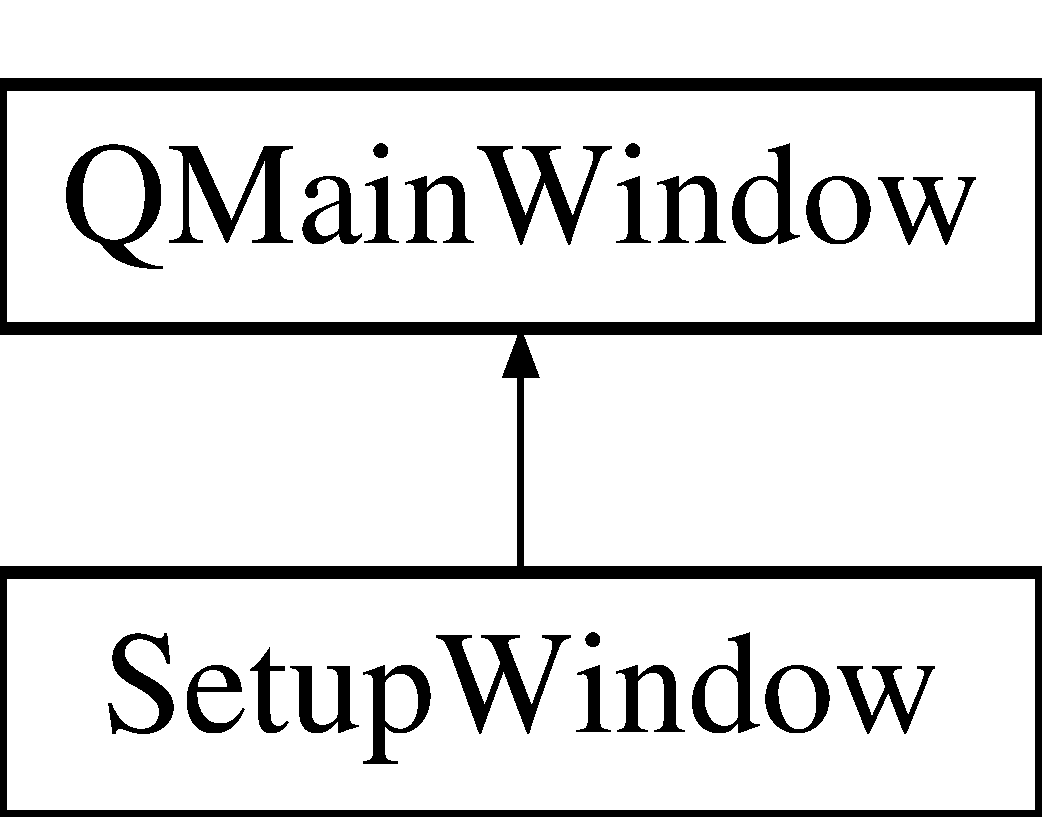
\includegraphics[height=2.000000cm]{class_setup_window}
\end{center}
\end{figure}
\subsection*{Öffentliche Methoden}
\begin{DoxyCompactItemize}
\item 
\hyperlink{class_setup_window_ae347da397b49800fca6a95c28a971acf}{Setup\+Window} (Q\+Widget $\ast$parent=0)
\begin{DoxyCompactList}\small\item\em Konstruktor zum Erzeugen einer Setup\+Window-\/\+Instanz. \end{DoxyCompactList}\item 
\hyperlink{class_setup_window_a5f825603c8e001970506c52be4755fd8}{$\sim$\+Setup\+Window} ()
\begin{DoxyCompactList}\small\item\em Destruktor zum Aufräumen einer Setup\+Window-\/\+Instanz. \end{DoxyCompactList}\end{DoxyCompactItemize}


\subsection{Ausführliche Beschreibung}
Die Klasse \hyperlink{class_setup_window}{Setup\+Window} ist ein kleiner Einrichtungsassistent, um ein Spiel zu konfigurieren. 

\subsection{Beschreibung der Konstruktoren und Destruktoren}
\hypertarget{class_setup_window_ae347da397b49800fca6a95c28a971acf}{}\index{Setup\+Window@{Setup\+Window}!Setup\+Window@{Setup\+Window}}
\index{Setup\+Window@{Setup\+Window}!Setup\+Window@{Setup\+Window}}
\subsubsection[{Setup\+Window}]{\setlength{\rightskip}{0pt plus 5cm}Setup\+Window\+::\+Setup\+Window (
\begin{DoxyParamCaption}
\item[{Q\+Widget $\ast$}]{parent = {\ttfamily 0}}
\end{DoxyParamCaption}
)\hspace{0.3cm}{\ttfamily [explicit]}}\label{class_setup_window_ae347da397b49800fca6a95c28a971acf}


Konstruktor zum Erzeugen einer Setup\+Window-\/\+Instanz. 


\begin{DoxyParams}{Parameter}
{\em parent} & Elternteil des Setup\+Windows \\
\hline
\end{DoxyParams}
\hypertarget{class_setup_window_a5f825603c8e001970506c52be4755fd8}{}\index{Setup\+Window@{Setup\+Window}!````~Setup\+Window@{$\sim$\+Setup\+Window}}
\index{````~Setup\+Window@{$\sim$\+Setup\+Window}!Setup\+Window@{Setup\+Window}}
\subsubsection[{$\sim$\+Setup\+Window}]{\setlength{\rightskip}{0pt plus 5cm}Setup\+Window\+::$\sim$\+Setup\+Window (
\begin{DoxyParamCaption}
{}
\end{DoxyParamCaption}
)}\label{class_setup_window_a5f825603c8e001970506c52be4755fd8}


Destruktor zum Aufräumen einer Setup\+Window-\/\+Instanz. 



Die Dokumentation für diese Klasse wurde erzeugt aufgrund der Dateien\+:\begin{DoxyCompactItemize}
\item 
src/\hyperlink{setupwindow_8hpp}{setupwindow.\+hpp}\item 
src/\hyperlink{setupwindow_8cpp}{setupwindow.\+cpp}\end{DoxyCompactItemize}

\hypertarget{class_window}{}\section{Window Klassenreferenz}
\label{class_window}\index{Window@{Window}}


Die Singleton-\/\+Klasse \hyperlink{class_window}{Window} ist die Haupt\+G\+U\+I.~\newline
 Dort findet das Spiel so wirklich für die Spieler statt.  




{\ttfamily \#include $<$window.\+hpp$>$}

Klassendiagramm für Window\+:\begin{figure}[H]
\begin{center}
\leavevmode
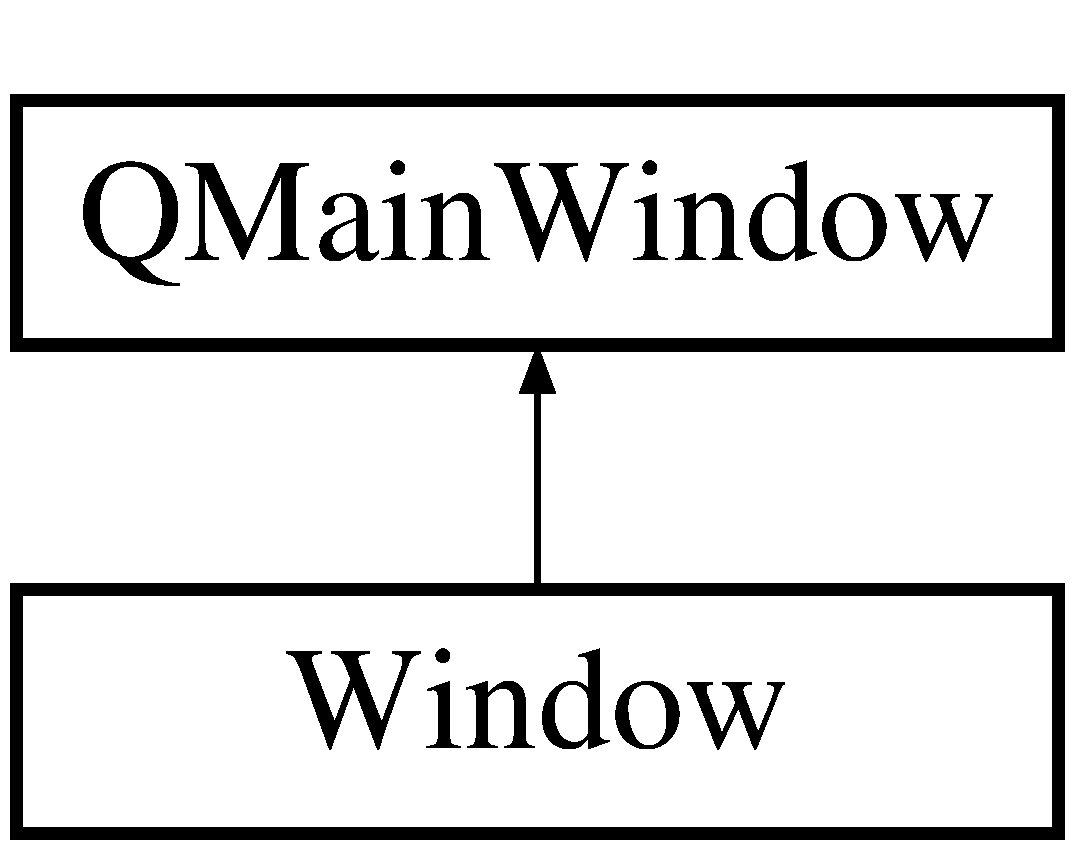
\includegraphics[height=2.000000cm]{class_window}
\end{center}
\end{figure}
\subsection*{Öffentliche Slots}
\begin{DoxyCompactItemize}
\item 
void \hyperlink{class_window_a5b62d2f0db72e3aad9d9b434fb692099}{card\+Clicked} ()
\begin{DoxyCompactList}\small\item\em Wird aufgerufen, wenn eine Karte angeklickt wird. \end{DoxyCompactList}\item 
void \hyperlink{class_window_acbd3c3b8edec3bd791c9f8d3e1ed3042}{client\+Disconnected} ()
\begin{DoxyCompactList}\small\item\em Wird aufgerufen, wenn die Verbindung zum \hyperlink{class_server}{Server} unterbrochen/ getrennt wird. \end{DoxyCompactList}\item 
void \hyperlink{class_window_a0c75a360bfab238425c2e0616151fb56}{retrieve\+Field} (Q\+Byte\+Array p\+\_\+field)
\begin{DoxyCompactList}\small\item\em Wird aufgerufen, wenn das Spielfeldsynchronisations-\/\+Paket empfangen wird. \end{DoxyCompactList}\item 
void \hyperlink{class_window_af7ad0380c530c760cf23a63a41dc47f6}{retrieve\+Deck\+Length} (short p\+\_\+deck\+Length)
\begin{DoxyCompactList}\small\item\em Wird aufgerufen, wenn das Deckgröße-\/\+Paket empfangen wird. \end{DoxyCompactList}\item 
void \hyperlink{class_window_a4f216b408b601635457f24f1662cb07b}{retrieve\+Scores} (Q\+Byte\+Array p\+\_\+scores)
\begin{DoxyCompactList}\small\item\em Wird aufgerufen, wenn das Punktestand-\/\+Paket empfangen wird. \end{DoxyCompactList}\item 
void \hyperlink{class_window_a9ee18fce7c1aa1c4699b2e279b71f3a8}{retrieve\+Game\+Started} ()
\begin{DoxyCompactList}\small\item\em Wird aufgerufen, wenn das Spielstarten-\/\+Paket empfangen wird. \end{DoxyCompactList}\item 
void \hyperlink{class_window_ae8cc4019b78c72f11011af84c2f7dd5a}{retrieve\+Game\+Finished} ()
\begin{DoxyCompactList}\small\item\em Wird aufgerufen, wenn das Spielbeenden-\/\+Paket empfangen wird. \end{DoxyCompactList}\item 
void \hyperlink{class_window_ab182caf7adf8a0227b8758cc37127b10}{retrieve\+Show\+Start\+Button} ()
\begin{DoxyCompactList}\small\item\em Wird aufgerufen, wenn der Start-\/\+Button angezeigt werden soll. \end{DoxyCompactList}\item 
void \hyperlink{class_window_a73d77bc7266516a16a9cdeb35db957f5}{retrieve\+Unlock} ()
\begin{DoxyCompactList}\small\item\em Wird aufgerufen, wenn das Eingabenentsperr-\/\+Paket emfpangen wird. \end{DoxyCompactList}\item 
void \hyperlink{class_window_a3b749278c0ca463b77df58e7e946142f}{retrieve\+Lock} ()
\begin{DoxyCompactList}\small\item\em Wird aufgerufen, wenn das Eingabesperr-\/\+Paket empfangen wird. \end{DoxyCompactList}\end{DoxyCompactItemize}
\subsection*{Signale}
\begin{DoxyCompactItemize}
\item 
void \hyperlink{class_window_aeec812dd91b692fd9b28296aae58dd22}{unselect\+All} ()
\begin{DoxyCompactList}\small\item\em Signal das alle Karten entwählt. \end{DoxyCompactList}\item 
void \hyperlink{class_window_ab5e88ca55b5471f875b222ed853a4e4e}{can\+Click} (bool p\+\_\+val)
\begin{DoxyCompactList}\small\item\em Signal das den Status der Karten -\/ ob man diese anklicken kann oder nicht -\/ festlegt. \end{DoxyCompactList}\end{DoxyCompactItemize}
\subsection*{Öffentliche, statische Methoden}
\begin{DoxyCompactItemize}
\item 
static \hyperlink{class_window}{Window} \& \hyperlink{class_window_a27532de1433b896e6586c3a9e045349d}{get\+Instance} ()
\begin{DoxyCompactList}\small\item\em Liefert die Instanz der Singleton-\/\+Klasse \hyperlink{class_window}{Window}. \end{DoxyCompactList}\end{DoxyCompactItemize}
\subsection*{Öffentliche Attribute}
\begin{DoxyCompactItemize}
\item 
std\+::list$<$ std\+::tuple$<$ \hyperlink{class_player}{Player} $\ast$, Qt\+::\+Key $>$ $>$ \hyperlink{class_window_af408d7d1516a7352c3076e71b8fad7d9}{m\+\_\+players}
\begin{DoxyCompactList}\small\item\em Liste aus allen aktuellen, lokalen Spielern und deren ausgewählte Taste. \end{DoxyCompactList}\end{DoxyCompactItemize}
\subsection*{Geschützte Methoden}
\begin{DoxyCompactItemize}
\item 
void \hyperlink{class_window_abbf36419d16aa9effd72df4fd8a742fe}{close\+Event} (Q\+Close\+Event $\ast$p\+\_\+close\+Event)
\begin{DoxyCompactList}\small\item\em Wird aufgerufen, wenn der Schließen-\/\+Button des Fensters geklickt wird. \end{DoxyCompactList}\item 
void \hyperlink{class_window_a580e4141cd01cb4d6d203cfe5c56352b}{key\+Press\+Event} (Q\+Key\+Event $\ast$p\+\_\+key\+Event)
\begin{DoxyCompactList}\small\item\em Wird aufgerufen, wenn eine Taste auf der Tastatur gedrückt wird. \end{DoxyCompactList}\end{DoxyCompactItemize}


\subsection{Ausführliche Beschreibung}
Die Singleton-\/\+Klasse \hyperlink{class_window}{Window} ist die Haupt\+G\+U\+I.~\newline
 Dort findet das Spiel so wirklich für die Spieler statt. 

\subsection{Dokumentation der Elementfunktionen}
\hypertarget{class_window_ab5e88ca55b5471f875b222ed853a4e4e}{}\index{Window@{Window}!can\+Click@{can\+Click}}
\index{can\+Click@{can\+Click}!Window@{Window}}
\subsubsection[{can\+Click}]{\setlength{\rightskip}{0pt plus 5cm}void Window\+::can\+Click (
\begin{DoxyParamCaption}
\item[{bool}]{p\+\_\+val}
\end{DoxyParamCaption}
)\hspace{0.3cm}{\ttfamily [signal]}}\label{class_window_ab5e88ca55b5471f875b222ed853a4e4e}


Signal das den Status der Karten -\/ ob man diese anklicken kann oder nicht -\/ festlegt. 


\begin{DoxyParams}{Parameter}
{\em p\+\_\+val} & Wahrheitswert der angibt, ob die Karten anklickbar sind oder nicht \\
\hline
\end{DoxyParams}
\hypertarget{class_window_a5b62d2f0db72e3aad9d9b434fb692099}{}\index{Window@{Window}!card\+Clicked@{card\+Clicked}}
\index{card\+Clicked@{card\+Clicked}!Window@{Window}}
\subsubsection[{card\+Clicked}]{\setlength{\rightskip}{0pt plus 5cm}void Window\+::card\+Clicked (
\begin{DoxyParamCaption}
{}
\end{DoxyParamCaption}
)\hspace{0.3cm}{\ttfamily [slot]}}\label{class_window_a5b62d2f0db72e3aad9d9b434fb692099}


Wird aufgerufen, wenn eine Karte angeklickt wird. 

\begin{DoxySeeAlso}{Siehe auch}
\hyperlink{class_card_widget_ab3f3a9b457b76a117c218cc1993ee1e4}{Card\+Widget\+::clicked} 
\end{DoxySeeAlso}
\hypertarget{class_window_acbd3c3b8edec3bd791c9f8d3e1ed3042}{}\index{Window@{Window}!client\+Disconnected@{client\+Disconnected}}
\index{client\+Disconnected@{client\+Disconnected}!Window@{Window}}
\subsubsection[{client\+Disconnected}]{\setlength{\rightskip}{0pt plus 5cm}void Window\+::client\+Disconnected (
\begin{DoxyParamCaption}
{}
\end{DoxyParamCaption}
)\hspace{0.3cm}{\ttfamily [slot]}}\label{class_window_acbd3c3b8edec3bd791c9f8d3e1ed3042}


Wird aufgerufen, wenn die Verbindung zum \hyperlink{class_server}{Server} unterbrochen/ getrennt wird. 

\hypertarget{class_window_abbf36419d16aa9effd72df4fd8a742fe}{}\index{Window@{Window}!close\+Event@{close\+Event}}
\index{close\+Event@{close\+Event}!Window@{Window}}
\subsubsection[{close\+Event}]{\setlength{\rightskip}{0pt plus 5cm}void Window\+::close\+Event (
\begin{DoxyParamCaption}
\item[{Q\+Close\+Event $\ast$}]{p\+\_\+close\+Event}
\end{DoxyParamCaption}
)\hspace{0.3cm}{\ttfamily [protected]}}\label{class_window_abbf36419d16aa9effd72df4fd8a742fe}


Wird aufgerufen, wenn der Schließen-\/\+Button des Fensters geklickt wird. 


\begin{DoxyParams}{Parameter}
{\em p\+\_\+close\+Event} & Schließ-\/\+Event \\
\hline
\end{DoxyParams}
\hypertarget{class_window_a27532de1433b896e6586c3a9e045349d}{}\index{Window@{Window}!get\+Instance@{get\+Instance}}
\index{get\+Instance@{get\+Instance}!Window@{Window}}
\subsubsection[{get\+Instance}]{\setlength{\rightskip}{0pt plus 5cm}{\bf Window} \& Window\+::get\+Instance (
\begin{DoxyParamCaption}
{}
\end{DoxyParamCaption}
)\hspace{0.3cm}{\ttfamily [static]}}\label{class_window_a27532de1433b896e6586c3a9e045349d}


Liefert die Instanz der Singleton-\/\+Klasse \hyperlink{class_window}{Window}. 

\begin{DoxyReturn}{Rückgabe}
Window-\/\+Instanz 
\end{DoxyReturn}
\hypertarget{class_window_a580e4141cd01cb4d6d203cfe5c56352b}{}\index{Window@{Window}!key\+Press\+Event@{key\+Press\+Event}}
\index{key\+Press\+Event@{key\+Press\+Event}!Window@{Window}}
\subsubsection[{key\+Press\+Event}]{\setlength{\rightskip}{0pt plus 5cm}void Window\+::key\+Press\+Event (
\begin{DoxyParamCaption}
\item[{Q\+Key\+Event $\ast$}]{p\+\_\+key\+Event}
\end{DoxyParamCaption}
)\hspace{0.3cm}{\ttfamily [protected]}}\label{class_window_a580e4141cd01cb4d6d203cfe5c56352b}


Wird aufgerufen, wenn eine Taste auf der Tastatur gedrückt wird. 


\begin{DoxyParams}{Parameter}
{\em p\+\_\+key\+Event} & Tasten-\/\+Event \\
\hline
\end{DoxyParams}
\hypertarget{class_window_af7ad0380c530c760cf23a63a41dc47f6}{}\index{Window@{Window}!retrieve\+Deck\+Length@{retrieve\+Deck\+Length}}
\index{retrieve\+Deck\+Length@{retrieve\+Deck\+Length}!Window@{Window}}
\subsubsection[{retrieve\+Deck\+Length}]{\setlength{\rightskip}{0pt plus 5cm}void Window\+::retrieve\+Deck\+Length (
\begin{DoxyParamCaption}
\item[{short}]{p\+\_\+deck\+Length}
\end{DoxyParamCaption}
)\hspace{0.3cm}{\ttfamily [slot]}}\label{class_window_af7ad0380c530c760cf23a63a41dc47f6}


Wird aufgerufen, wenn das Deckgröße-\/\+Paket empfangen wird. 


\begin{DoxyParams}{Parameter}
{\em p\+\_\+deck\+Length} & Deckgröße \\
\hline
\end{DoxyParams}
\begin{DoxySeeAlso}{Siehe auch}
\hyperlink{class_packet_handler_abc467ba059a00877d8fae31672395ac4}{Packet\+Handler\+::read\+Deck\+Length} 
\end{DoxySeeAlso}
\hypertarget{class_window_a0c75a360bfab238425c2e0616151fb56}{}\index{Window@{Window}!retrieve\+Field@{retrieve\+Field}}
\index{retrieve\+Field@{retrieve\+Field}!Window@{Window}}
\subsubsection[{retrieve\+Field}]{\setlength{\rightskip}{0pt plus 5cm}void Window\+::retrieve\+Field (
\begin{DoxyParamCaption}
\item[{Q\+Byte\+Array}]{p\+\_\+field}
\end{DoxyParamCaption}
)\hspace{0.3cm}{\ttfamily [slot]}}\label{class_window_a0c75a360bfab238425c2e0616151fb56}


Wird aufgerufen, wenn das Spielfeldsynchronisations-\/\+Paket empfangen wird. 


\begin{DoxyParams}{Parameter}
{\em p\+\_\+field} & Spielfeld \\
\hline
\end{DoxyParams}
\begin{DoxySeeAlso}{Siehe auch}
\hyperlink{class_packet_handler_a7434b94845f0389703fa4d85e8487372}{Packet\+Handler\+::read\+Field} 
\end{DoxySeeAlso}
\hypertarget{class_window_ae8cc4019b78c72f11011af84c2f7dd5a}{}\index{Window@{Window}!retrieve\+Game\+Finished@{retrieve\+Game\+Finished}}
\index{retrieve\+Game\+Finished@{retrieve\+Game\+Finished}!Window@{Window}}
\subsubsection[{retrieve\+Game\+Finished}]{\setlength{\rightskip}{0pt plus 5cm}void Window\+::retrieve\+Game\+Finished (
\begin{DoxyParamCaption}
{}
\end{DoxyParamCaption}
)\hspace{0.3cm}{\ttfamily [slot]}}\label{class_window_ae8cc4019b78c72f11011af84c2f7dd5a}


Wird aufgerufen, wenn das Spielbeenden-\/\+Paket empfangen wird. 

\begin{DoxySeeAlso}{Siehe auch}
\hyperlink{class_packet_handler_aa47688eb98584d262f5ba2f98f019105}{Packet\+Handler\+::read\+Game\+Finished\+Packet} 
\end{DoxySeeAlso}
\hypertarget{class_window_a9ee18fce7c1aa1c4699b2e279b71f3a8}{}\index{Window@{Window}!retrieve\+Game\+Started@{retrieve\+Game\+Started}}
\index{retrieve\+Game\+Started@{retrieve\+Game\+Started}!Window@{Window}}
\subsubsection[{retrieve\+Game\+Started}]{\setlength{\rightskip}{0pt plus 5cm}void Window\+::retrieve\+Game\+Started (
\begin{DoxyParamCaption}
{}
\end{DoxyParamCaption}
)\hspace{0.3cm}{\ttfamily [slot]}}\label{class_window_a9ee18fce7c1aa1c4699b2e279b71f3a8}


Wird aufgerufen, wenn das Spielstarten-\/\+Paket empfangen wird. 

\begin{DoxySeeAlso}{Siehe auch}
\hyperlink{class_packet_handler_a84c59146583fc6ee254940cce4377b54}{Packet\+Handler\+::read\+Game\+Started\+Packet} 
\end{DoxySeeAlso}
\hypertarget{class_window_a3b749278c0ca463b77df58e7e946142f}{}\index{Window@{Window}!retrieve\+Lock@{retrieve\+Lock}}
\index{retrieve\+Lock@{retrieve\+Lock}!Window@{Window}}
\subsubsection[{retrieve\+Lock}]{\setlength{\rightskip}{0pt plus 5cm}void Window\+::retrieve\+Lock (
\begin{DoxyParamCaption}
{}
\end{DoxyParamCaption}
)\hspace{0.3cm}{\ttfamily [slot]}}\label{class_window_a3b749278c0ca463b77df58e7e946142f}


Wird aufgerufen, wenn das Eingabesperr-\/\+Paket empfangen wird. 

\begin{DoxySeeAlso}{Siehe auch}
\hyperlink{class_packet_handler_acba72c3a586146653ad0b6c0851dbc0c}{Packet\+Handler\+::read\+Locked\+Packet} 
\end{DoxySeeAlso}
\hypertarget{class_window_a4f216b408b601635457f24f1662cb07b}{}\index{Window@{Window}!retrieve\+Scores@{retrieve\+Scores}}
\index{retrieve\+Scores@{retrieve\+Scores}!Window@{Window}}
\subsubsection[{retrieve\+Scores}]{\setlength{\rightskip}{0pt plus 5cm}void Window\+::retrieve\+Scores (
\begin{DoxyParamCaption}
\item[{Q\+Byte\+Array}]{p\+\_\+scores}
\end{DoxyParamCaption}
)\hspace{0.3cm}{\ttfamily [slot]}}\label{class_window_a4f216b408b601635457f24f1662cb07b}


Wird aufgerufen, wenn das Punktestand-\/\+Paket empfangen wird. 


\begin{DoxyParams}{Parameter}
{\em p\+\_\+scores} & Punktestand \\
\hline
\end{DoxyParams}
\begin{DoxySeeAlso}{Siehe auch}
\hyperlink{class_packet_handler_a766789a5ff926bee167e308b620f8807}{Packet\+Handler\+::read\+Scores} 
\end{DoxySeeAlso}
\hypertarget{class_window_ab182caf7adf8a0227b8758cc37127b10}{}\index{Window@{Window}!retrieve\+Show\+Start\+Button@{retrieve\+Show\+Start\+Button}}
\index{retrieve\+Show\+Start\+Button@{retrieve\+Show\+Start\+Button}!Window@{Window}}
\subsubsection[{retrieve\+Show\+Start\+Button}]{\setlength{\rightskip}{0pt plus 5cm}void Window\+::retrieve\+Show\+Start\+Button (
\begin{DoxyParamCaption}
{}
\end{DoxyParamCaption}
)\hspace{0.3cm}{\ttfamily [slot]}}\label{class_window_ab182caf7adf8a0227b8758cc37127b10}


Wird aufgerufen, wenn der Start-\/\+Button angezeigt werden soll. 

\begin{DoxySeeAlso}{Siehe auch}
\hyperlink{class_controller_a7b451f4eb09398e825910d02e73f8789}{Controller\+::show\+Start\+Button} 
\end{DoxySeeAlso}
\hypertarget{class_window_a73d77bc7266516a16a9cdeb35db957f5}{}\index{Window@{Window}!retrieve\+Unlock@{retrieve\+Unlock}}
\index{retrieve\+Unlock@{retrieve\+Unlock}!Window@{Window}}
\subsubsection[{retrieve\+Unlock}]{\setlength{\rightskip}{0pt plus 5cm}void Window\+::retrieve\+Unlock (
\begin{DoxyParamCaption}
{}
\end{DoxyParamCaption}
)\hspace{0.3cm}{\ttfamily [slot]}}\label{class_window_a73d77bc7266516a16a9cdeb35db957f5}


Wird aufgerufen, wenn das Eingabenentsperr-\/\+Paket emfpangen wird. 

\begin{DoxySeeAlso}{Siehe auch}
\hyperlink{class_packet_handler_a309f2c1cd016039c1fe8b38d75b3ef7c}{Packet\+Handler\+::read\+Unlocked\+Packet} 
\end{DoxySeeAlso}
\hypertarget{class_window_aeec812dd91b692fd9b28296aae58dd22}{}\index{Window@{Window}!unselect\+All@{unselect\+All}}
\index{unselect\+All@{unselect\+All}!Window@{Window}}
\subsubsection[{unselect\+All}]{\setlength{\rightskip}{0pt plus 5cm}void Window\+::unselect\+All (
\begin{DoxyParamCaption}
{}
\end{DoxyParamCaption}
)\hspace{0.3cm}{\ttfamily [signal]}}\label{class_window_aeec812dd91b692fd9b28296aae58dd22}


Signal das alle Karten entwählt. 



\subsection{Dokumentation der Datenelemente}
\hypertarget{class_window_af408d7d1516a7352c3076e71b8fad7d9}{}\index{Window@{Window}!m\+\_\+players@{m\+\_\+players}}
\index{m\+\_\+players@{m\+\_\+players}!Window@{Window}}
\subsubsection[{m\+\_\+players}]{\setlength{\rightskip}{0pt plus 5cm}std\+::list$<$std\+::tuple$<${\bf Player}$\ast$, Qt\+::\+Key$>$ $>$ Window\+::m\+\_\+players}\label{class_window_af408d7d1516a7352c3076e71b8fad7d9}


Liste aus allen aktuellen, lokalen Spielern und deren ausgewählte Taste. 



Die Dokumentation für diese Klasse wurde erzeugt aufgrund der Dateien\+:\begin{DoxyCompactItemize}
\item 
src/\hyperlink{window_8hpp}{window.\+hpp}\item 
src/\hyperlink{window_8cpp}{window.\+cpp}\end{DoxyCompactItemize}

\chapter{Datei-\/\+Dokumentation}
\hypertarget{card_8cpp}{}\section{src/card.cpp-\/\+Dateireferenz}
\label{card_8cpp}\index{src/card.\+cpp@{src/card.\+cpp}}
{\ttfamily \#include \char`\"{}card.\+hpp\char`\"{}}\\*

\hypertarget{card_8hpp}{}\section{src/card.hpp-\/\+Dateireferenz}
\label{card_8hpp}\index{src/card.\+hpp@{src/card.\+hpp}}
{\ttfamily \#include \char`\"{}enums.\+hpp\char`\"{}}\\*
{\ttfamily \#include \char`\"{}cardwidget.\+hpp\char`\"{}}\\*
{\ttfamily \#include \char`\"{}window.\+hpp\char`\"{}}\\*
{\ttfamily \#include \char`\"{}controller.\+hpp\char`\"{}}\\*
\subsection*{Klassen}
\begin{DoxyCompactItemize}
\item 
class \hyperlink{class_card}{Card}
\begin{DoxyCompactList}\small\item\em Die Klasse \hyperlink{class_card}{Card} stellt das digitale pendant zu den analogen Karten des Spiels Set dar. \end{DoxyCompactList}\end{DoxyCompactItemize}

\hypertarget{cardwidget_8cpp}{}\section{src/cardwidget.cpp-\/\+Dateireferenz}
\label{cardwidget_8cpp}\index{src/cardwidget.\+cpp@{src/cardwidget.\+cpp}}
{\ttfamily \#include \char`\"{}cardwidget.\+hpp\char`\"{}}\\*

\hypertarget{cardwidget_8hpp}{}\section{src/cardwidget.hpp-\/\+Dateireferenz}
\label{cardwidget_8hpp}\index{src/cardwidget.\+hpp@{src/cardwidget.\+hpp}}
{\ttfamily \#include $<$atomic$>$}\\*
{\ttfamily \#include $<$Q\+Widget$>$}\\*
{\ttfamily \#include $<$Q\+Painter$>$}\\*
{\ttfamily \#include $<$Q\+Paint\+Event$>$}\\*
{\ttfamily \#include $<$Q\+Mouse\+Event$>$}\\*
{\ttfamily \#include \char`\"{}card.\+hpp\char`\"{}}\\*
\subsection*{Klassen}
\begin{DoxyCompactItemize}
\item 
class \hyperlink{class_card_widget}{Card\+Widget}
\begin{DoxyCompactList}\small\item\em Die grafische Implementierung der Klasse \hyperlink{class_card}{Card}. \end{DoxyCompactList}\end{DoxyCompactItemize}

\hypertarget{client_8cpp}{}\section{src/client.cpp-\/\+Dateireferenz}
\label{client_8cpp}\index{src/client.\+cpp@{src/client.\+cpp}}
{\ttfamily \#include \char`\"{}client.\+hpp\char`\"{}}\\*

\hypertarget{client_8hpp}{}\section{src/client.hpp-\/\+Dateireferenz}
\label{client_8hpp}\index{src/client.\+hpp@{src/client.\+hpp}}
{\ttfamily \#include $<$Q\+Tcp\+Socket$>$}\\*
{\ttfamily \#include $<$Q\+Host\+Address$>$}\\*
{\ttfamily \#include \char`\"{}packethandler.\+hpp\char`\"{}}\\*
\subsection*{Klassen}
\begin{DoxyCompactItemize}
\item 
class \hyperlink{class_client}{Client}
\begin{DoxyCompactList}\small\item\em Die abstrakte Klasse \hyperlink{class_client}{Client} kümmert sich um die Verbindung zum \hyperlink{class_server}{Server} und macht so ein Spielen möglich. \end{DoxyCompactList}\end{DoxyCompactItemize}

\hypertarget{controller_8cpp}{}\section{src/controller.cpp-\/\+Dateireferenz}
\label{controller_8cpp}\index{src/controller.\+cpp@{src/controller.\+cpp}}
{\ttfamily \#include \char`\"{}controller.\+hpp\char`\"{}}\\*

\hypertarget{controller_8hpp}{}\section{src/controller.hpp-\/\+Dateireferenz}
\label{controller_8hpp}\index{src/controller.\+hpp@{src/controller.\+hpp}}
{\ttfamily \#include $<$atomic$>$}\\*
{\ttfamily \#include $<$list$>$}\\*
{\ttfamily \#include $<$stdlib.\+h$>$}\\*
{\ttfamily \#include $<$ctime$>$}\\*
{\ttfamily \#include $<$thread$>$}\\*
{\ttfamily \#include $<$chrono$>$}\\*
{\ttfamily \#include $<$Q\+Timer$>$}\\*
{\ttfamily \#include \char`\"{}server.\+hpp\char`\"{}}\\*
{\ttfamily \#include \char`\"{}card.\+hpp\char`\"{}}\\*
\subsection*{Klassen}
\begin{DoxyCompactItemize}
\item 
class \hyperlink{class_controller}{Controller}
\begin{DoxyCompactList}\small\item\em Die Klasse \hyperlink{class_controller}{Controller} ist für den kompletten Spielverlauf zuständig.~\newline
 Sie regelt, wann welcher \hyperlink{class_client}{Client} welche Pakete empfängt, wann das Spiel zu Ende ist/anfängt und~\newline
 wenn Karten nachgelegt werden sollen. \end{DoxyCompactList}\end{DoxyCompactItemize}

\hypertarget{enums_8hpp}{}\section{src/enums.hpp-\/\+Dateireferenz}
\label{enums_8hpp}\index{src/enums.\+hpp@{src/enums.\+hpp}}
{\ttfamily \#include $<$Q\+Color$>$}\\*
\subsection*{Aufzählungen}
\begin{DoxyCompactItemize}
\item 
enum \hyperlink{enums_8hpp_aadfc99008cde4759cbc40855d1aceae0}{Packet\+Header} \{ \\*
\hyperlink{enums_8hpp_aadfc99008cde4759cbc40855d1aceae0ae07d0fb3d06a8c0fe90def87455acb2d}{G\+A\+M\+E\+\_\+\+S\+T\+A\+T\+E} = 0x01, 
\hyperlink{enums_8hpp_aadfc99008cde4759cbc40855d1aceae0a938d82cfb3bdc31f73ca0dcd969ad4d6}{D\+E\+C\+K} = 0x02, 
\hyperlink{enums_8hpp_aadfc99008cde4759cbc40855d1aceae0ac51b9561ae664fd1616bb7d0827b7247}{I\+N\+P\+U\+T\+\_\+\+S\+T\+A\+T\+E} = 0x03, 
\hyperlink{enums_8hpp_aadfc99008cde4759cbc40855d1aceae0a074bbf7a9f1fc57292380e29fb6323de}{P\+L\+A\+Y\+E\+R\+\_\+\+T\+U\+R\+N} = 0x04, 
\\*
\hyperlink{enums_8hpp_aadfc99008cde4759cbc40855d1aceae0a90001ad69ab9874fbdfbbae899a92b1a}{S\+C\+O\+R\+E\+S} = 0x05, 
\hyperlink{enums_8hpp_aadfc99008cde4759cbc40855d1aceae0a7c774fbaf120abe58ef0a79fe384e6e4}{F\+I\+E\+L\+D\+\_\+\+S\+Y\+N\+C\+H\+R\+O} = 0x07, 
\hyperlink{enums_8hpp_aadfc99008cde4759cbc40855d1aceae0ab03e8ec91b0d074a03df67327675f025}{C\+L\+I\+C\+K} = 0x0\+A
 \}
\begin{DoxyCompactList}\small\item\em Anonyme innere Klasse, mit den verschiedenen Pakettypen. \end{DoxyCompactList}\item 
enum \hyperlink{enums_8hpp_ab87bacfdad76e61b9412d7124be44c1c}{Color} \{ \hyperlink{enums_8hpp_ab87bacfdad76e61b9412d7124be44c1caf80f9a890089d211842d59625e561f88}{R\+E\+D}, 
\hyperlink{enums_8hpp_ab87bacfdad76e61b9412d7124be44c1ca35d6719cb4d7577c031b3d79057a1b79}{B\+L\+U\+E}, 
\hyperlink{enums_8hpp_ab87bacfdad76e61b9412d7124be44c1caa60bd322f93178d68184e30e162571ca}{G\+R\+E\+E\+N}
 \}
\begin{DoxyCompactList}\small\item\em Anonyme innere Klasse, mit den verschiedenen Farben einer Karte. \end{DoxyCompactList}\item 
enum \hyperlink{enums_8hpp_a55b506070847a13554f8b879c1bfb37c}{Shape} \{ \hyperlink{enums_8hpp_a55b506070847a13554f8b879c1bfb37ca2fd33892864d1c342d3bead2f2d9ad56}{T\+R\+I\+A\+N\+G\+L\+E}, 
\hyperlink{enums_8hpp_a55b506070847a13554f8b879c1bfb37ca4233fbf0cafb86abcee94b38d769fc59}{S\+Q\+U\+A\+R\+E}, 
\hyperlink{enums_8hpp_a55b506070847a13554f8b879c1bfb37caa79c827759ea48f0735386c4b1188911}{C\+I\+R\+C\+L\+E}
 \}
\begin{DoxyCompactList}\small\item\em Anonyme innere Klasse, mit den verschiedenen Formen einer Karte. \end{DoxyCompactList}\item 
enum \hyperlink{enums_8hpp_ad1fb407b73d9c6e54eec2180d3bc4d48}{Number} \{ \hyperlink{enums_8hpp_ad1fb407b73d9c6e54eec2180d3bc4d48a7a725f13af144bdef532d0389ba75e0d}{O\+N\+E}, 
\hyperlink{enums_8hpp_ad1fb407b73d9c6e54eec2180d3bc4d48a0e793500a63ffa575b9b712ca3bc9851}{T\+W\+O}, 
\hyperlink{enums_8hpp_ad1fb407b73d9c6e54eec2180d3bc4d48a1251fbf93888ad32fe0ae54d49bcef17}{T\+H\+R\+E\+E}
 \}
\begin{DoxyCompactList}\small\item\em Anonyme innere Klasse, mit den verschiedenen Anzahlen einer Karte. \end{DoxyCompactList}\item 
enum \hyperlink{enums_8hpp_a31841bed26ecf2fc5a6253eb838aac4b}{Opacity} \{ \hyperlink{enums_8hpp_a31841bed26ecf2fc5a6253eb838aac4ba535cbdd94e9f2a4c67f6c5a7a7b16311}{F\+I\+L\+L\+E\+D}, 
\hyperlink{enums_8hpp_a31841bed26ecf2fc5a6253eb838aac4ba2f0d18fc0d0fa4a6cd92dc328501874d}{E\+M\+P\+T\+Y}, 
\hyperlink{enums_8hpp_a31841bed26ecf2fc5a6253eb838aac4ba1f517a44fd9145c222e62c03e2f40b4b}{P\+A\+L\+L\+I\+D}
 \}
\begin{DoxyCompactList}\small\item\em Anonyme innere Klasse, mit den verschiedenen Einfärbungen einer Karte. \end{DoxyCompactList}\end{DoxyCompactItemize}


\subsection{Dokumentation der Aufzählungstypen}
\hypertarget{enums_8hpp_ab87bacfdad76e61b9412d7124be44c1c}{}\index{enums.\+hpp@{enums.\+hpp}!Color@{Color}}
\index{Color@{Color}!enums.\+hpp@{enums.\+hpp}}
\subsubsection[{Color}]{\setlength{\rightskip}{0pt plus 5cm}enum {\bf Color}}\label{enums_8hpp_ab87bacfdad76e61b9412d7124be44c1c}


Anonyme innere Klasse, mit den verschiedenen Farben einer Karte. 

\begin{Desc}
\item[Aufzählungswerte]\par
\begin{description}
\index{R\+E\+D@{R\+E\+D}!enums.\+hpp@{enums.\+hpp}}\index{enums.\+hpp@{enums.\+hpp}!R\+E\+D@{R\+E\+D}}\item[{\em 
\hypertarget{enums_8hpp_ab87bacfdad76e61b9412d7124be44c1caf80f9a890089d211842d59625e561f88}{}R\+E\+D\label{enums_8hpp_ab87bacfdad76e61b9412d7124be44c1caf80f9a890089d211842d59625e561f88}
}]\index{B\+L\+U\+E@{B\+L\+U\+E}!enums.\+hpp@{enums.\+hpp}}\index{enums.\+hpp@{enums.\+hpp}!B\+L\+U\+E@{B\+L\+U\+E}}\item[{\em 
\hypertarget{enums_8hpp_ab87bacfdad76e61b9412d7124be44c1ca35d6719cb4d7577c031b3d79057a1b79}{}B\+L\+U\+E\label{enums_8hpp_ab87bacfdad76e61b9412d7124be44c1ca35d6719cb4d7577c031b3d79057a1b79}
}]\index{G\+R\+E\+E\+N@{G\+R\+E\+E\+N}!enums.\+hpp@{enums.\+hpp}}\index{enums.\+hpp@{enums.\+hpp}!G\+R\+E\+E\+N@{G\+R\+E\+E\+N}}\item[{\em 
\hypertarget{enums_8hpp_ab87bacfdad76e61b9412d7124be44c1caa60bd322f93178d68184e30e162571ca}{}G\+R\+E\+E\+N\label{enums_8hpp_ab87bacfdad76e61b9412d7124be44c1caa60bd322f93178d68184e30e162571ca}
}]\end{description}
\end{Desc}
\hypertarget{enums_8hpp_ad1fb407b73d9c6e54eec2180d3bc4d48}{}\index{enums.\+hpp@{enums.\+hpp}!Number@{Number}}
\index{Number@{Number}!enums.\+hpp@{enums.\+hpp}}
\subsubsection[{Number}]{\setlength{\rightskip}{0pt plus 5cm}enum {\bf Number}}\label{enums_8hpp_ad1fb407b73d9c6e54eec2180d3bc4d48}


Anonyme innere Klasse, mit den verschiedenen Anzahlen einer Karte. 

\begin{Desc}
\item[Aufzählungswerte]\par
\begin{description}
\index{O\+N\+E@{O\+N\+E}!enums.\+hpp@{enums.\+hpp}}\index{enums.\+hpp@{enums.\+hpp}!O\+N\+E@{O\+N\+E}}\item[{\em 
\hypertarget{enums_8hpp_ad1fb407b73d9c6e54eec2180d3bc4d48a7a725f13af144bdef532d0389ba75e0d}{}O\+N\+E\label{enums_8hpp_ad1fb407b73d9c6e54eec2180d3bc4d48a7a725f13af144bdef532d0389ba75e0d}
}]\index{T\+W\+O@{T\+W\+O}!enums.\+hpp@{enums.\+hpp}}\index{enums.\+hpp@{enums.\+hpp}!T\+W\+O@{T\+W\+O}}\item[{\em 
\hypertarget{enums_8hpp_ad1fb407b73d9c6e54eec2180d3bc4d48a0e793500a63ffa575b9b712ca3bc9851}{}T\+W\+O\label{enums_8hpp_ad1fb407b73d9c6e54eec2180d3bc4d48a0e793500a63ffa575b9b712ca3bc9851}
}]\index{T\+H\+R\+E\+E@{T\+H\+R\+E\+E}!enums.\+hpp@{enums.\+hpp}}\index{enums.\+hpp@{enums.\+hpp}!T\+H\+R\+E\+E@{T\+H\+R\+E\+E}}\item[{\em 
\hypertarget{enums_8hpp_ad1fb407b73d9c6e54eec2180d3bc4d48a1251fbf93888ad32fe0ae54d49bcef17}{}T\+H\+R\+E\+E\label{enums_8hpp_ad1fb407b73d9c6e54eec2180d3bc4d48a1251fbf93888ad32fe0ae54d49bcef17}
}]\end{description}
\end{Desc}
\hypertarget{enums_8hpp_a31841bed26ecf2fc5a6253eb838aac4b}{}\index{enums.\+hpp@{enums.\+hpp}!Opacity@{Opacity}}
\index{Opacity@{Opacity}!enums.\+hpp@{enums.\+hpp}}
\subsubsection[{Opacity}]{\setlength{\rightskip}{0pt plus 5cm}enum {\bf Opacity}}\label{enums_8hpp_a31841bed26ecf2fc5a6253eb838aac4b}


Anonyme innere Klasse, mit den verschiedenen Einfärbungen einer Karte. 

\begin{Desc}
\item[Aufzählungswerte]\par
\begin{description}
\index{F\+I\+L\+L\+E\+D@{F\+I\+L\+L\+E\+D}!enums.\+hpp@{enums.\+hpp}}\index{enums.\+hpp@{enums.\+hpp}!F\+I\+L\+L\+E\+D@{F\+I\+L\+L\+E\+D}}\item[{\em 
\hypertarget{enums_8hpp_a31841bed26ecf2fc5a6253eb838aac4ba535cbdd94e9f2a4c67f6c5a7a7b16311}{}F\+I\+L\+L\+E\+D\label{enums_8hpp_a31841bed26ecf2fc5a6253eb838aac4ba535cbdd94e9f2a4c67f6c5a7a7b16311}
}]\index{E\+M\+P\+T\+Y@{E\+M\+P\+T\+Y}!enums.\+hpp@{enums.\+hpp}}\index{enums.\+hpp@{enums.\+hpp}!E\+M\+P\+T\+Y@{E\+M\+P\+T\+Y}}\item[{\em 
\hypertarget{enums_8hpp_a31841bed26ecf2fc5a6253eb838aac4ba2f0d18fc0d0fa4a6cd92dc328501874d}{}E\+M\+P\+T\+Y\label{enums_8hpp_a31841bed26ecf2fc5a6253eb838aac4ba2f0d18fc0d0fa4a6cd92dc328501874d}
}]\index{P\+A\+L\+L\+I\+D@{P\+A\+L\+L\+I\+D}!enums.\+hpp@{enums.\+hpp}}\index{enums.\+hpp@{enums.\+hpp}!P\+A\+L\+L\+I\+D@{P\+A\+L\+L\+I\+D}}\item[{\em 
\hypertarget{enums_8hpp_a31841bed26ecf2fc5a6253eb838aac4ba1f517a44fd9145c222e62c03e2f40b4b}{}P\+A\+L\+L\+I\+D\label{enums_8hpp_a31841bed26ecf2fc5a6253eb838aac4ba1f517a44fd9145c222e62c03e2f40b4b}
}]\end{description}
\end{Desc}
\hypertarget{enums_8hpp_aadfc99008cde4759cbc40855d1aceae0}{}\index{enums.\+hpp@{enums.\+hpp}!Packet\+Header@{Packet\+Header}}
\index{Packet\+Header@{Packet\+Header}!enums.\+hpp@{enums.\+hpp}}
\subsubsection[{Packet\+Header}]{\setlength{\rightskip}{0pt plus 5cm}enum {\bf Packet\+Header}}\label{enums_8hpp_aadfc99008cde4759cbc40855d1aceae0}


Anonyme innere Klasse, mit den verschiedenen Pakettypen. 

\begin{Desc}
\item[Aufzählungswerte]\par
\begin{description}
\index{G\+A\+M\+E\+\_\+\+S\+T\+A\+T\+E@{G\+A\+M\+E\+\_\+\+S\+T\+A\+T\+E}!enums.\+hpp@{enums.\+hpp}}\index{enums.\+hpp@{enums.\+hpp}!G\+A\+M\+E\+\_\+\+S\+T\+A\+T\+E@{G\+A\+M\+E\+\_\+\+S\+T\+A\+T\+E}}\item[{\em 
\hypertarget{enums_8hpp_aadfc99008cde4759cbc40855d1aceae0ae07d0fb3d06a8c0fe90def87455acb2d}{}G\+A\+M\+E\+\_\+\+S\+T\+A\+T\+E\label{enums_8hpp_aadfc99008cde4759cbc40855d1aceae0ae07d0fb3d06a8c0fe90def87455acb2d}
}]\index{D\+E\+C\+K@{D\+E\+C\+K}!enums.\+hpp@{enums.\+hpp}}\index{enums.\+hpp@{enums.\+hpp}!D\+E\+C\+K@{D\+E\+C\+K}}\item[{\em 
\hypertarget{enums_8hpp_aadfc99008cde4759cbc40855d1aceae0a938d82cfb3bdc31f73ca0dcd969ad4d6}{}D\+E\+C\+K\label{enums_8hpp_aadfc99008cde4759cbc40855d1aceae0a938d82cfb3bdc31f73ca0dcd969ad4d6}
}]\index{I\+N\+P\+U\+T\+\_\+\+S\+T\+A\+T\+E@{I\+N\+P\+U\+T\+\_\+\+S\+T\+A\+T\+E}!enums.\+hpp@{enums.\+hpp}}\index{enums.\+hpp@{enums.\+hpp}!I\+N\+P\+U\+T\+\_\+\+S\+T\+A\+T\+E@{I\+N\+P\+U\+T\+\_\+\+S\+T\+A\+T\+E}}\item[{\em 
\hypertarget{enums_8hpp_aadfc99008cde4759cbc40855d1aceae0ac51b9561ae664fd1616bb7d0827b7247}{}I\+N\+P\+U\+T\+\_\+\+S\+T\+A\+T\+E\label{enums_8hpp_aadfc99008cde4759cbc40855d1aceae0ac51b9561ae664fd1616bb7d0827b7247}
}]\index{P\+L\+A\+Y\+E\+R\+\_\+\+T\+U\+R\+N@{P\+L\+A\+Y\+E\+R\+\_\+\+T\+U\+R\+N}!enums.\+hpp@{enums.\+hpp}}\index{enums.\+hpp@{enums.\+hpp}!P\+L\+A\+Y\+E\+R\+\_\+\+T\+U\+R\+N@{P\+L\+A\+Y\+E\+R\+\_\+\+T\+U\+R\+N}}\item[{\em 
\hypertarget{enums_8hpp_aadfc99008cde4759cbc40855d1aceae0a074bbf7a9f1fc57292380e29fb6323de}{}P\+L\+A\+Y\+E\+R\+\_\+\+T\+U\+R\+N\label{enums_8hpp_aadfc99008cde4759cbc40855d1aceae0a074bbf7a9f1fc57292380e29fb6323de}
}]\index{S\+C\+O\+R\+E\+S@{S\+C\+O\+R\+E\+S}!enums.\+hpp@{enums.\+hpp}}\index{enums.\+hpp@{enums.\+hpp}!S\+C\+O\+R\+E\+S@{S\+C\+O\+R\+E\+S}}\item[{\em 
\hypertarget{enums_8hpp_aadfc99008cde4759cbc40855d1aceae0a90001ad69ab9874fbdfbbae899a92b1a}{}S\+C\+O\+R\+E\+S\label{enums_8hpp_aadfc99008cde4759cbc40855d1aceae0a90001ad69ab9874fbdfbbae899a92b1a}
}]\index{F\+I\+E\+L\+D\+\_\+\+S\+Y\+N\+C\+H\+R\+O@{F\+I\+E\+L\+D\+\_\+\+S\+Y\+N\+C\+H\+R\+O}!enums.\+hpp@{enums.\+hpp}}\index{enums.\+hpp@{enums.\+hpp}!F\+I\+E\+L\+D\+\_\+\+S\+Y\+N\+C\+H\+R\+O@{F\+I\+E\+L\+D\+\_\+\+S\+Y\+N\+C\+H\+R\+O}}\item[{\em 
\hypertarget{enums_8hpp_aadfc99008cde4759cbc40855d1aceae0a7c774fbaf120abe58ef0a79fe384e6e4}{}F\+I\+E\+L\+D\+\_\+\+S\+Y\+N\+C\+H\+R\+O\label{enums_8hpp_aadfc99008cde4759cbc40855d1aceae0a7c774fbaf120abe58ef0a79fe384e6e4}
}]\index{C\+L\+I\+C\+K@{C\+L\+I\+C\+K}!enums.\+hpp@{enums.\+hpp}}\index{enums.\+hpp@{enums.\+hpp}!C\+L\+I\+C\+K@{C\+L\+I\+C\+K}}\item[{\em 
\hypertarget{enums_8hpp_aadfc99008cde4759cbc40855d1aceae0ab03e8ec91b0d074a03df67327675f025}{}C\+L\+I\+C\+K\label{enums_8hpp_aadfc99008cde4759cbc40855d1aceae0ab03e8ec91b0d074a03df67327675f025}
}]\end{description}
\end{Desc}
\hypertarget{enums_8hpp_a55b506070847a13554f8b879c1bfb37c}{}\index{enums.\+hpp@{enums.\+hpp}!Shape@{Shape}}
\index{Shape@{Shape}!enums.\+hpp@{enums.\+hpp}}
\subsubsection[{Shape}]{\setlength{\rightskip}{0pt plus 5cm}enum {\bf Shape}}\label{enums_8hpp_a55b506070847a13554f8b879c1bfb37c}


Anonyme innere Klasse, mit den verschiedenen Formen einer Karte. 

\begin{Desc}
\item[Aufzählungswerte]\par
\begin{description}
\index{T\+R\+I\+A\+N\+G\+L\+E@{T\+R\+I\+A\+N\+G\+L\+E}!enums.\+hpp@{enums.\+hpp}}\index{enums.\+hpp@{enums.\+hpp}!T\+R\+I\+A\+N\+G\+L\+E@{T\+R\+I\+A\+N\+G\+L\+E}}\item[{\em 
\hypertarget{enums_8hpp_a55b506070847a13554f8b879c1bfb37ca2fd33892864d1c342d3bead2f2d9ad56}{}T\+R\+I\+A\+N\+G\+L\+E\label{enums_8hpp_a55b506070847a13554f8b879c1bfb37ca2fd33892864d1c342d3bead2f2d9ad56}
}]\index{S\+Q\+U\+A\+R\+E@{S\+Q\+U\+A\+R\+E}!enums.\+hpp@{enums.\+hpp}}\index{enums.\+hpp@{enums.\+hpp}!S\+Q\+U\+A\+R\+E@{S\+Q\+U\+A\+R\+E}}\item[{\em 
\hypertarget{enums_8hpp_a55b506070847a13554f8b879c1bfb37ca4233fbf0cafb86abcee94b38d769fc59}{}S\+Q\+U\+A\+R\+E\label{enums_8hpp_a55b506070847a13554f8b879c1bfb37ca4233fbf0cafb86abcee94b38d769fc59}
}]\index{C\+I\+R\+C\+L\+E@{C\+I\+R\+C\+L\+E}!enums.\+hpp@{enums.\+hpp}}\index{enums.\+hpp@{enums.\+hpp}!C\+I\+R\+C\+L\+E@{C\+I\+R\+C\+L\+E}}\item[{\em 
\hypertarget{enums_8hpp_a55b506070847a13554f8b879c1bfb37caa79c827759ea48f0735386c4b1188911}{}C\+I\+R\+C\+L\+E\label{enums_8hpp_a55b506070847a13554f8b879c1bfb37caa79c827759ea48f0735386c4b1188911}
}]\end{description}
\end{Desc}

\hypertarget{informationwidget_8cpp}{}\section{src/informationwidget.cpp-\/\+Dateireferenz}
\label{informationwidget_8cpp}\index{src/informationwidget.\+cpp@{src/informationwidget.\+cpp}}
{\ttfamily \#include \char`\"{}informationwidget.\+hpp\char`\"{}}\\*

\hypertarget{informationwidget_8hpp}{}\section{src/informationwidget.hpp-\/\+Dateireferenz}
\label{informationwidget_8hpp}\index{src/informationwidget.\+hpp@{src/informationwidget.\+hpp}}
{\ttfamily \#include $<$iostream$>$}\\*
{\ttfamily \#include $<$Q\+Widget$>$}\\*
{\ttfamily \#include $<$Q\+Label$>$}\\*
\subsection*{Klassen}
\begin{DoxyCompactItemize}
\item 
class \hyperlink{class_information_widget}{Information\+Widget}
\begin{DoxyCompactList}\small\item\em Das \hyperlink{class_information_widget}{Information\+Widget} dient zur Ausgabe des Spielstatuses. \end{DoxyCompactList}\end{DoxyCompactItemize}

\hypertarget{ki_8cpp}{}\section{src/ki.cpp-\/\+Dateireferenz}
\label{ki_8cpp}\index{src/ki.\+cpp@{src/ki.\+cpp}}
{\ttfamily \#include \char`\"{}ki.\+hpp\char`\"{}}\\*

\hypertarget{ki_8hpp}{}\section{src/ki.hpp-\/\+Dateireferenz}
\label{ki_8hpp}\index{src/ki.\+hpp@{src/ki.\+hpp}}
{\ttfamily \#include $<$atomic$>$}\\*
{\ttfamily \#include $<$thread$>$}\\*
{\ttfamily \#include $<$mutex$>$}\\*
{\ttfamily \#include $<$chrono$>$}\\*
{\ttfamily \#include \char`\"{}player.\+hpp\char`\"{}}\\*
{\ttfamily \#include \char`\"{}card.\+hpp\char`\"{}}\\*
\subsection*{Klassen}
\begin{DoxyCompactItemize}
\item 
class \hyperlink{class_k_i}{K\+I}
\end{DoxyCompactItemize}

\hypertarget{main_8cpp}{}\section{src/main.cpp-\/\+Dateireferenz}
\label{main_8cpp}\index{src/main.\+cpp@{src/main.\+cpp}}
{\ttfamily \#include $<$Q\+Application$>$}\\*
{\ttfamily \#include \char`\"{}setupwindow.\+hpp\char`\"{}}\\*
\subsection*{Funktionen}
\begin{DoxyCompactItemize}
\item 
int \hyperlink{main_8cpp_a0ddf1224851353fc92bfbff6f499fa97}{main} (int argc, char $\ast$argv\mbox{[}$\,$\mbox{]})
\end{DoxyCompactItemize}


\subsection{Dokumentation der Funktionen}
\hypertarget{main_8cpp_a0ddf1224851353fc92bfbff6f499fa97}{}\index{main.\+cpp@{main.\+cpp}!main@{main}}
\index{main@{main}!main.\+cpp@{main.\+cpp}}
\subsubsection[{main}]{\setlength{\rightskip}{0pt plus 5cm}int main (
\begin{DoxyParamCaption}
\item[{int}]{argc, }
\item[{char $\ast$}]{argv\mbox{[}$\,$\mbox{]}}
\end{DoxyParamCaption}
)}\label{main_8cpp_a0ddf1224851353fc92bfbff6f499fa97}

\hypertarget{packethandler_8cpp}{}\section{src/packethandler.cpp-\/\+Dateireferenz}
\label{packethandler_8cpp}\index{src/packethandler.\+cpp@{src/packethandler.\+cpp}}
{\ttfamily \#include \char`\"{}packethandler.\+hpp\char`\"{}}\\*

\hypertarget{packethandler_8hpp}{}\section{src/packethandler.hpp-\/\+Dateireferenz}
\label{packethandler_8hpp}\index{src/packethandler.\+hpp@{src/packethandler.\+hpp}}
{\ttfamily \#include $<$iostream$>$}\\*
{\ttfamily \#include $<$Q\+Object$>$}\\*
{\ttfamily \#include $<$Q\+Tcp\+Socket$>$}\\*
{\ttfamily \#include \char`\"{}enums.\+hpp\char`\"{}}\\*
{\ttfamily \#include \char`\"{}card.\+hpp\char`\"{}}\\*
\subsection*{Klassen}
\begin{DoxyCompactItemize}
\item 
class \hyperlink{class_packet_handler}{Packet\+Handler}
\begin{DoxyCompactList}\small\item\em Die Packet\+Handler-\/\+Klasse dient zur Verwaltung von ein-\/ bzw. ausgehenden Paketen.~\newline
 Werden bestimmte Pakettypen erkannt, so werden die entsprechenden Signale emittiert,~\newline
 und dadurch die Slots in den externen Klassen aufgerufen. \end{DoxyCompactList}\end{DoxyCompactItemize}

\hypertarget{player_8cpp}{}\section{src/player.cpp-\/\+Dateireferenz}
\label{player_8cpp}\index{src/player.\+cpp@{src/player.\+cpp}}
{\ttfamily \#include \char`\"{}player.\+hpp\char`\"{}}\\*

\hypertarget{player_8hpp}{}\section{src/player.hpp-\/\+Dateireferenz}
\label{player_8hpp}\index{src/player.\+hpp@{src/player.\+hpp}}
{\ttfamily \#include $<$Q\+Object$>$}\\*
{\ttfamily \#include $<$Q\+Byte\+Array$>$}\\*
{\ttfamily \#include \char`\"{}client.\+hpp\char`\"{}}\\*
\subsection*{Klassen}
\begin{DoxyCompactItemize}
\item 
class \hyperlink{class_player}{Player}
\begin{DoxyCompactList}\small\item\em Spieler-\/\+Klasse. \end{DoxyCompactList}\end{DoxyCompactItemize}

\hypertarget{server_8cpp}{}\section{src/server.cpp-\/\+Dateireferenz}
\label{server_8cpp}\index{src/server.\+cpp@{src/server.\+cpp}}
{\ttfamily \#include \char`\"{}server.\+hpp\char`\"{}}\\*

\hypertarget{server_8hpp}{}\section{src/server.hpp-\/\+Dateireferenz}
\label{server_8hpp}\index{src/server.\+hpp@{src/server.\+hpp}}
{\ttfamily \#include $<$vector$>$}\\*
{\ttfamily \#include $<$tuple$>$}\\*
{\ttfamily \#include $<$Q\+Tcp\+Server$>$}\\*
{\ttfamily \#include \char`\"{}packethandler.\+hpp\char`\"{}}\\*
\subsection*{Klassen}
\begin{DoxyCompactItemize}
\item 
class \hyperlink{class_server}{Server}
\begin{DoxyCompactList}\small\item\em Die abstrakte Klasse \hyperlink{class_server}{Server}, steht für den \hyperlink{class_server}{Server} des Spiels. \end{DoxyCompactList}\end{DoxyCompactItemize}

\hypertarget{setupwindow_8cpp}{}\section{src/setupwindow.cpp-\/\+Dateireferenz}
\label{setupwindow_8cpp}\index{src/setupwindow.\+cpp@{src/setupwindow.\+cpp}}
{\ttfamily \#include \char`\"{}src/setupwindow.\+hpp\char`\"{}}\\*
{\ttfamily \#include \char`\"{}ui\+\_\+setupwindow.\+h\char`\"{}}\\*

\hypertarget{setupwindow_8hpp}{}\section{src/setupwindow.hpp-\/\+Dateireferenz}
\label{setupwindow_8hpp}\index{src/setupwindow.\+hpp@{src/setupwindow.\+hpp}}
{\ttfamily \#include $<$iostream$>$}\\*
{\ttfamily \#include $<$Q\+Main\+Window$>$}\\*
{\ttfamily \#include $<$Q\+List\+Widget\+Item$>$}\\*
{\ttfamily \#include $<$Q\+Key\+Event$>$}\\*
{\ttfamily \#include $<$Q\+Desktop\+Widget$>$}\\*
{\ttfamily \#include \char`\"{}window.\+hpp\char`\"{}}\\*
{\ttfamily \#include \char`\"{}player.\+hpp\char`\"{}}\\*
{\ttfamily \#include \char`\"{}ki.\+hpp\char`\"{}}\\*
{\ttfamily \#include \char`\"{}controller.\+hpp\char`\"{}}\\*
\subsection*{Klassen}
\begin{DoxyCompactItemize}
\item 
class \hyperlink{class_setup_window}{Setup\+Window}
\begin{DoxyCompactList}\small\item\em Die Klasse \hyperlink{class_setup_window}{Setup\+Window} ist ein kleiner Einrichtungsassistent, um ein Spiel zu konfigurieren. \end{DoxyCompactList}\end{DoxyCompactItemize}
\subsection*{Namensbereiche}
\begin{DoxyCompactItemize}
\item 
 \hyperlink{namespace_ui}{Ui}
\end{DoxyCompactItemize}

\hypertarget{window_8cpp}{}\section{src/window.cpp-\/\+Dateireferenz}
\label{window_8cpp}\index{src/window.\+cpp@{src/window.\+cpp}}
{\ttfamily \#include \char`\"{}window.\+hpp\char`\"{}}\\*
{\ttfamily \#include \char`\"{}ui\+\_\+window.\+h\char`\"{}}\\*

\hypertarget{window_8hpp}{}\section{src/window.hpp-\/\+Dateireferenz}
\label{window_8hpp}\index{src/window.\+hpp@{src/window.\+hpp}}
{\ttfamily \#include $<$atomic$>$}\\*
{\ttfamily \#include $<$list$>$}\\*
{\ttfamily \#include $<$Q\+Desktop\+Widget$>$}\\*
{\ttfamily \#include $<$Q\+Main\+Window$>$}\\*
{\ttfamily \#include $<$Q\+Widget$>$}\\*
{\ttfamily \#include $<$Q\+Push\+Button$>$}\\*
{\ttfamily \#include $<$Q\+Message\+Box$>$}\\*
{\ttfamily \#include $<$Q\+Key\+Event$>$}\\*
{\ttfamily \#include \char`\"{}card.\+hpp\char`\"{}}\\*
{\ttfamily \#include \char`\"{}informationwidget.\+hpp\char`\"{}}\\*
{\ttfamily \#include \char`\"{}player.\+hpp\char`\"{}}\\*
{\ttfamily \#include \char`\"{}controller.\+hpp\char`\"{}}\\*
\subsection*{Klassen}
\begin{DoxyCompactItemize}
\item 
class \hyperlink{class_window}{Window}
\begin{DoxyCompactList}\small\item\em Die Singleton-\/\+Klasse \hyperlink{class_window}{Window} ist die Haupt\+G\+U\+I.~\newline
 Dort findet das Spiel so wirklich für die Spieler statt. \end{DoxyCompactList}\end{DoxyCompactItemize}
\subsection*{Namensbereiche}
\begin{DoxyCompactItemize}
\item 
 \hyperlink{namespace_ui}{Ui}
\end{DoxyCompactItemize}

%--- End generated contents ---

% Index
\backmatter
\newpage
\phantomsection
\clearemptydoublepage
\addcontentsline{toc}{chapter}{Index}
\printindex

\end{document}
